\documentclass[12pt,notitlepage]{report}
\usepackage{cite}					%bibliography
\usepackage{mathptmx}				%Times New Roman
\usepackage{geometry}				% Margins
 \geometry{
 a4paper,
 total={210mm,297mm},
 left=20mm,
 right=20mm,
 top=20mm,
 bottom=20mm,
 bindingoffset=0mm
 }
\usepackage[utf8]{inputenc}
\usepackage{tikz}
\usepackage{float}
\usepackage[ruled,vlined,noend]{algorithm2e}
\usepackage{caption}
\usepackage{subcaption}
\usepackage[english]{babel}
\usepackage{amssymb}
\usepackage{amsmath}
\DeclareMathOperator*{\argmin}{argmin}

\usepackage{tikz-uml}
\usepackage{graphicx}
\usepackage{fancybox}
\newcommand{\shadowpicture}[1]{%
  \shadowsize=1pt
  \fboxrule=0pt
  \fboxsep=0pt
  \color{gray}
  \shadowbox{\fboxsep=6pt\fcolorbox{white}{white}{#1}}
  \normalcolor
}

\usepackage{xcolor}
\usepackage{listings}
\lstset{language=java, frame=single,framesep=\fboxsep,framerule=\fboxrule,
rulecolor=\color{red},backgroundcolor=\color{yellow!5},basicstyle=\footnotesize\tt,tabsize=1,
numbersep=5mm, numbers=none,numberstyle=\footnotesize,keywordstyle=\color{blue}\sf,identifierstyle=\color{magenta},showstringspaces=false}

\usepackage[T1]{fontenc}
\usepackage{titlesec, blindtext, color}
\definecolor{gray75}{gray}{0.75}
\newcommand{\hsp}{\hspace{20pt}}
\titleformat{\chapter}[hang]{\Huge\bfseries}{\thechapter\hsp\textcolor{gray75}{|}\hsp}{0pt}{\Huge\bfseries}

\usepackage{todonotes}

\usepackage{booktabs}
\usepackage{tabularx}
\newcolumntype{L}[1]{>{\raggedright\arraybackslash}p{#1}}
\newcolumntype{C}[1]{>{\centering\arraybackslash}p{#1}}
\newcolumntype{R}[1]{>{\raggedleft\arraybackslash}p{#1}}
\usepackage{colortbl}

\usepackage{url}  %for URL in bibliography
\usepackage[justification=centering]{caption}

\begin{document}

%%%%%%%%%%%%%%%%%%%%%%%%%%%%%%%%%%%%%%%%%%%%%%%%%%%%%%%%%%%%%%%%%%%%%%%%
% Title


\pagestyle{empty}

\hfill{\LARGE \bf Oliver Freeman}

\vspace*{60mm}
\begin{center}
\Huge
{\bf A comparison of \\Any-Angle Pathfinding Algorithms \\for Virtual Agents} \\
\vspace*{5mm}
Computer Science: Part II \\
\vspace*{5mm}
Clare College \\
\vspace*{5mm}
\today  % today's date
\end{center}

\cleardoublepage

%%%%%%%%%%%%%%%%%%%%%%%%%%%%%%%%%%%%%%%%%%%%%%%%%%%%%%%%%%%%%%%%%%%%%%%%%%%%%%
% Proforma, table of contents and list of figures

\setcounter{page}{1}
\pagenumbering{roman}
\pagestyle{plain}

\chapter*{Proforma}

{\large
\begin{tabular}{ll}
Name:               & \bf Oliver Freeman                      \\
College:            & \bf Clare College                    \\
Project Title:      & \bf A comparison of Any-Angle Pathfinding\\ 
                    & \bf Algorithms for Virtual Agents \\
Examination:        & \bf Computer Science Tripos: Part II, May 2014        \\
Word Count:         & \bf 11,944\footnotemark[1]\\
Project Originator: & \bf Oliver Freeman                   \\
Supervisor:         & \bf Dr. R. J. Gibbens                   \\ 
\end{tabular}
}

\footnotetext[1]{This word count was computed by {\tt detex of209dissertation.tex | tr -cd `0-9-Za-z \textbackslash n' | wc -w}.} 


\section*{Original Aims of the Project}

The aims of this project were to compare and contrast the structure and performance of a selection of recently published any-angle pathfinding algorithms.

\section*{Work Completed}
The pathfinding simulator allows a user to choose or create a map and specify any of the pathfinding algorithms to find a path through that map. The simulator displays the path found along with various statistics about that map. Statistics can be automatically generated for large volumes of maps using the simulator's API.\\

\noindent
Evaluation of the statistics produced by the simulator shows results consistent with the literature, and alternative implementation strategies are also compared. Discussion of the algorithms identifies shortcomings in common comparison metrics, and suggests possible optimisations for the algorithms.

\section*{Special Difficulties}
None.
 
\newpage
\section*{Declaration}

I, Oliver Freeman of Clare College, being a candidate for Part II of the Computer
Science Tripos, hereby declare that this dissertation and the work described in it are my own work,
unaided except as may be specified below, and that the dissertation
does not contain material that has already been used to any substantial
extent for a comparable purpose.

\bigskip
\leftline{Signed}

\medskip
\leftline{Date}

\cleardoublepage

\tableofcontents

\listoffigures

\listoftables

\listofalgorithms

%%%%%%%%%%%%%%%%%%%%%%%%%%%%%%%%%%%%%%%%%%%%%%%%%%%%%%%%%%%%%%%%%%%%%%%
% now for the chapters

\cleardoublepage        % just to make sure before the page numbering
                        % is changed

\setcounter{page}{1}
\pagenumbering{arabic}
\pagestyle{headings}

\chapter{Introduction}

\section{Motivation}

Finding short and realistic-looking paths through maps with arbitrarily placed obstacles is one of the central problems in artificial intelligence for games and robotics. Figure 1.1 (a) shows a grid-based map, consisting of free cells and blocked cells. Figure 1.1 (b) shows the shortest path through this map between the $start$ and the $goal$.\\

\noindent
However, pathfinding algorithms operate on graphs. A graph representation of this map is shown in figure 1.1 (c) --- each node in the graph represents a coordinate on the map, and an agent can travel directly between any two nodes connected by an edge. Figure 1.1 (d) shows the shortest path through the graph --- however, this is clearly longer than the optimum path through the map, shown in figure 1.1 (b).\\
\begin{figure}[h]
\centering
    \begin{tikzpicture}[scale=1.1,line width=0.5pt]
    
    \node (a) at (0,4) {
    \begin{tikzpicture}[scale=1.1,line width=0.5pt]
      \filldraw[color=black!60,fill=black!40] (1,1) rectangle (2,3); 
      \draw[color=black!60] (0,0) grid (3,3);
      \draw[black] (0,0) -- (3,0);
      \draw[black] (0,0) -- (0,3);
      \draw[black] (3,3) -- (3,0);
      \draw[black] (3,3) -- (0,3);
      
      \node[below] at (1.5,0) {(a)};
      \end{tikzpicture}
      };
      
     \node (b) at (6,4) {
      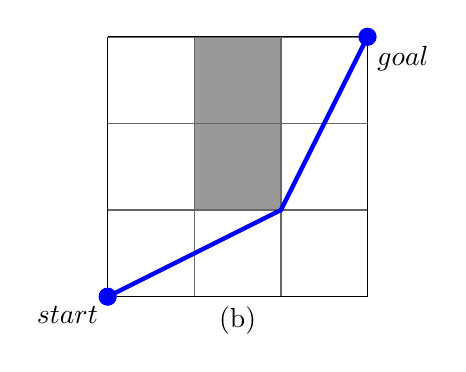
\begin{tikzpicture}[scale=1.1,line width=0.5pt]
      \filldraw[color=black!60,fill=black!40] (1,1) rectangle (2,3); 
      \draw[color=black!60] (0,0) grid (3,3);
      \draw[blue, ultra thick] (0,0) -- (2,1) -- (3,3); 
      
      \draw[black] (0,0) -- (3,0);
      \draw[black] (0,0) -- (0,3);
      \draw[black] (3,3) -- (3,0);
      \draw[black] (3,3) -- (0,3);
      
      \node[below right] at (3,3) {$goal$};
      \fill[blue] (3,3) circle (3pt);
      \node[below left] at (0,0) {$start$};
      \fill[blue] (0,0) circle (3pt);
      
      \node[below] at (1.5,0) {(b)};
      
      \end{tikzpicture}
      };
      
      \node (c) at (0,0) {
      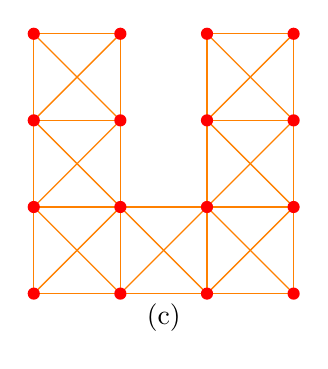
\begin{tikzpicture}[scale=1.1,line width=0.5pt]

     \draw[orange] (0,0) grid (3,3);
     
     \foreach \x in {0,1,2} {
        \foreach \y in {0,1,2} {
          \pgfmathparse{int(\x + 1)};
          \let\xa\pgfmathresult;
          \pgfmathparse{int(\y + 1)};
          \let\ya\pgfmathresult;
          \draw[orange] (\x,\y) -- (\xa,\ya);
        }
      }
  
      \foreach \x in {0,1,2} {
        \foreach \y in {1,2,3} {
          \pgfmathparse{int(\x + 1)};
          \let\xa\pgfmathresult;
          \pgfmathparse{int(\y - 1)};
          \let\ya\pgfmathresult;
          \draw[orange] (\x,\y) -- (\xa,\ya);
        }
      }
      
       \filldraw[color=orange,fill=white] (1,1) rectangle (2,3);
      \draw[white, ultra thick] (1,2) -- (2,2);
      \draw[white, ultra thick] (1,3) -- (2,3);

      \foreach \x in {0,1,2,3} {
        \foreach \y in {0,1,2,3} {
          \fill[red] (\x,\y) circle (2pt);
        }
      }
      
      \node[below] at (1.5,0) {(c)};
      \end{tikzpicture}
      };
      
      \node (d) at (6,0) {
      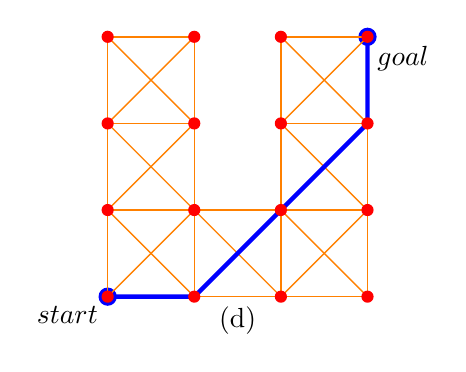
\begin{tikzpicture}[scale=1.1,line width=0.5pt]
    
      \fill[blue] (3,3) circle (3pt);
      \fill[blue] (0,0) circle (3pt);
      \draw[orange] (0,0) grid (3,3);
  
      \foreach \x in {0,1,2} {
        \foreach \y in {0,1,2} {
          \pgfmathparse{int(\x + 1)};
          \let\xa\pgfmathresult;
          \pgfmathparse{int(\y + 1)};
          \let\ya\pgfmathresult;
          \draw[orange] (\x,\y) -- (\xa,\ya);
        }
      }
  
      \foreach \x in {0,1,2} {
        \foreach \y in {1,2,3} {
          \pgfmathparse{int(\x + 1)};
          \let\xa\pgfmathresult;
          \pgfmathparse{int(\y - 1)};
          \let\ya\pgfmathresult;
          \draw[orange] (\x,\y) -- (\xa,\ya);
        }
      }

      \node[below right] at (3,3) {$goal$};
      \node[below left] at (0,0) {$start$};

      \draw[blue, ultra thick] (0,0) -- (1,0) -- (3,2) -- (3,3);
      
      \filldraw[color=orange,fill=white] (1,1) rectangle (2,3);
      \draw[white, ultra thick] (1,2) -- (2,2);
      \draw[white, ultra thick] (1,3) -- (2,3);

      \foreach \x in {0,1,2,3} {
        \foreach \y in {0,1,2,3} {
          \fill[red] (\x,\y) circle (2pt);
        }
      }
      \node[below] at (1.5,0) {(d)};
      \end{tikzpicture}
      };
      
      \node[left] at (-2,0.2) {node};
      \draw[->] (-2,0.2) -- (-1.55,0.75);
      \node[right] at (2,0.2) {edge};
      \draw[->] (2,0.2) -- (1.2,0.4);
      
      \node[left] at (-2,4.7) {free cell};
      \draw[->] (-2,4.7) -- (-1,5.3);
      \node[right] at (2,4) {blocked cell};
      \draw[->] (2,4) -- (0,4.4);
      
    \end{tikzpicture}
  \caption[Shortest paths through maps and graphs]{Shortest path through a map vs. shortest path through the graph representing the map}
 \label{fig:fart}
\end{figure}

\noindent
The structure of this graph is based on the grid structure of the map. If a different graph representation was chosen then a shorter path could have been achieved, but in general such a graph would require many more nodes and edges which would cause exponentially increasing memory requirements and search-space size. This dissertation will investigate various algorithms that aim to find a near-optimal path through a map while using space-efficient grid-based graph like that shown in Figure 1.1(c).\\

\section{Related work}

{\em A*} is a well known algorithm that finds optimal paths through graphs. Applying a post-processing step to smooth and hence shorten paths returned by {\em A*} is a technique that has been used since the earliest video games\cite{Thorpe84}, but most of the research into more advanced any-angle pathfinding algorithms have taken place in the last half decade. \\

\noindent
Ferguson and Stentz's paper on {\em Field D*}\cite{FergusonStentz06} in 2006 was followed by a significant contribution to the field by Nash and Koenig et al., who published papers on {\em Theta*}\cite{Daniel10} and {\em Lazy Theta*}\cite{Nash10} in 2010. In 2011, {\em Yap et al.}'s paper on {\em Block A*}\cite{Yap11} introduced the concept of pre-calculating solutions to sub-maps to speed up execution.\\

\noindent
Studies such as Nash and Koneig's article in {\em Artificial Intelligence Magazine}\cite{Nash13} have been conducted that compare a selection of these any-angle pathfinding algorithms. However, no paper has attempted to explain and compare these algorithms with a consistent framework, and the only established authority that utilises empirical data on {\em Block A*} is Yap et al.'s own work\cite{Yap11}\cite{Yap11_2}, which compares only {\em A*}, {\em Theta*} and {\em Block A*}.

\section {Project goals}

\noindent
The goals of this project are to:

\begin{itemize}
\item introduce a cohesive framework for explaining the most prominent any-angle path-finding algorithms;
\item create an algorithm simulation environment that enables intuitive and informative comparison of the performance of these algorithms;
\item use statistical analysis and explanations based on the framework to present conclusions on the performance of the algorithms that enhance those presented in the current literature.
\end {itemize}

\cleardoublepage


\chapter{Preparation} 

\section{Introduction to any-angle pathfinding}

This section formally introduces the concept of maps and describes how graphs are created from maps. It then defines the any-angle path-finding problem. A formal mathematical framework is defined throughout this section so that the any-angle pathfinding algorithms can be explained using a unifying graph-theoretic approach. Such an approach has not been attempted in any of the published papers on any-angle pathfinding algorithms.

\subsection{Map}

A map $M$ of size $N \times N$ is a square region in two-dimensional space $[0,N]^{2} \subseteq \mathbb{R}^{2}$, where $N \in\mathbb{Z^+}$. A location on the map can be specified with a coordinate $(x,y) \in M$.\\

\noindent
The map is logically divided into a grid of $N \times N$ cells of size $1 \times 1$, where cell $C_{i,j}$ includes all locations $(x,y) \in M$ where $i \leq x \leq i+1$ and $j \leq y \leq j+1$, and each cell is either `free' or `blocked'.\\

\begin{figure}
\centering
 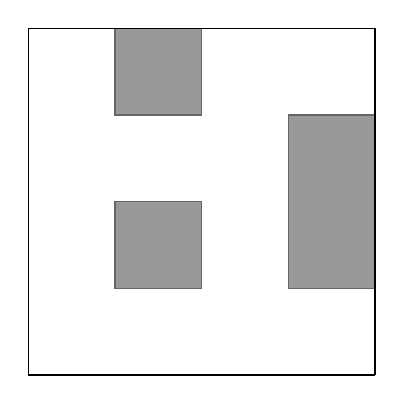
\begin{tikzpicture}[scale=1.1,line width=0.5pt]
      
      \filldraw[color=black!60,fill=black!40] (1,1) rectangle (2,2); 
      \filldraw[color=black!60,fill=black!40] (1,3) rectangle (2,4); 
      \filldraw[color=black!60,fill=black!40] (3,1) rectangle (4,3); 
      %\draw[color=black!60] (0,0) grid (4,4);
      
      \draw[black] (0,0) -- (4,0);
      \draw[black] (0,0) -- (0,4);
      \draw[black] (4,4) -- (4,0);
      \draw[black] (4,4) -- (0,4);
     
    \end{tikzpicture}
  \caption{A map of size $4^{2}$}
  %\label{fig:fig}
\end{figure}

\begin{description}
\item{\bfseries Valid location}\\
The agent is modelled as a dimensionless point, as is the convention\cite{Daniel10} in any-angle pathfinding research. Therefore, a valid location is defined as any location $(x,y) \in M$ that lies in a free cell or on the boundary of a free cell.\\

\item{\bfseries Line of sight}\\
A line of sight exists between two locations $(x_{0},y_{0})$ and $(x_{1},y_{1})$ on a map if all locations that lie on the straight line drawn between $(x_{0},y_{0})$ and $(x_{1},y_{1})$ are valid --- that is to say, for all $t \in \mathbb{R}$ where $0 \leq t \leq 1$: $(x_{0} + t(x_{1}-x_{0}),y_{0} + t(y_{1}-y_{0}))$ is a valid location. The existence of a line of sight between two locations implies that an agent can travel in a straight line between the two locations.\\

\item{\bfseries Path through a map}\\
A path  $P_{M} = ((x_{0},y_{0}), (x_{1},y_{1}), \ldots, (x_{n},y_{n}))$ through map $M$ is an ordered list of coordinates $(x,y) \in M$ where $(x_{0},y_{0})$ = $(x_{start},y_{start})$ is the $start$ location of the path, and $(x_{n},y_{n})$ = $(x_{goal},y_{goal})$ is the $goal$ location of the path. A path is valid if a line of sight exists between every sequential pair of coordinates in the path: $(x_{i},y_{i})$ and $(x_{i+1},y_{i+1})$.\\
\end{description}

\noindent
It should be noted that since the agent is modelled as a dimensionless point, the path through the map shown in Figure 2.2, which features a `diagonal blockage', is a valid path.\\

\begin{figure}
    \centering
    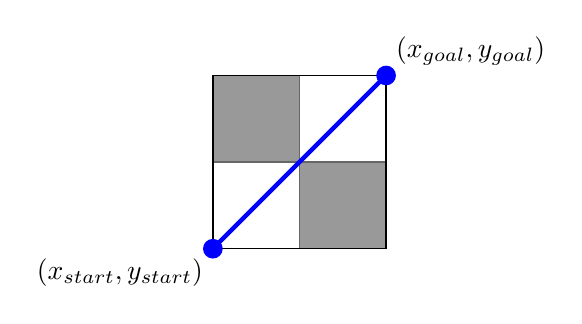
\begin{tikzpicture}[scale=1.1,line width=0.5pt]
      \filldraw[color=black!60,fill=black!40] (0,1) rectangle (1,2); 
      \filldraw[color=black!60,fill=black!40] (1,0) rectangle (2,1); 
      \draw (0,0) -- (2,0);
      \draw (0,0) -- (0,2);
      \draw (2,2) -- (2,0);
      \draw (2,2) -- (0,2);
      \node[below left] at (0,0) {$(x_{start},y_{start})$};
      \node[above right] at (2,2) {$(x_{goal},y_{goal})$};
      \filldraw[blue] (0,0) circle (3pt);
      \filldraw[blue] (2,2) circle (3pt);
      \draw[blue, ultra thick] (0,0) -- (2,2);
      
          
    \end{tikzpicture}
  \caption{A valid path for an agent modelled as a point}
  %\label{fig:fig}
\end{figure}

\subsection{Graph}

Pathfinding algorithms operate on graphs. Therefore, to find a path through a map between a given $start$ and $goal$, the following steps are taken:
\begin{enumerate}
\item a graph that represents the map is produced, where each node in the graph represents a location in the map; 
\item a pathfinding algorithm is applied to the graph, which returns a path through the graph;
\item this path through the graph corresponds to a path through the map.
\end{enumerate}
Step 1 is introduced in the upcoming `Discretisation' paragraph. Step 2 is introduced in section 2.2. Step 3 is a result of the definition of a graph, which now follows:\\

\noindent{\bfseries Graph}\\
\noindent
A graph $G(M)=(V,E)$ is a representation, or abstraction, of a map $M$. Each node $n \in V$ represents a valid location $(a,b) \in M$. If a line of sight exists between two locations in $M$ then the the two nodes $n$ and $n'$ that represent these locations are connected by an edge $e=(n,n') \in E$, thus called `neighbours'. $(n,n').weight$ is the distance an agent would traverse by travelling directly between the two locations i.e. the Euclidean distance between them.

\begin{description}
\item{\bfseries Path through a graph}\\
A path $P_{G(M)} = (n_{0}, n_{1}, \ldots, n_{n})$ through graph $G(M)=(V,E)$ is a list of nodes $n \in V$, where $n_{0}=n_{start}$ and $n_{n}=n_{goal}$. A path is valid if, for each pair of nodes $n_{i}$ and $n_{i+1}$, there exists an edge $(n_{i},n_{i+1}) \in E$.\\
\end{description}

\noindent
There are two types of graph:
\begin{enumerate}
\item{\bfseries Grid-based graph} $G_{g}(M)$ --- a node represents every valid location that lies on a corner of a cell in $M$. Each node is connected to each of the up to eight nodes that directly surround it\footnote{If node $n$ represents location $(i,j)$, the ``up to eight nodes that directly surround it'' are the nodes that represent the locations $(i-1,j-1)$, $(i-1,j)$, $(i-1,j+1)$, $(i,j+1)$, $(i+1,j+1)$, $(i+1,j)$, $(i+1,j-1)$ and $(i-1,j)$.} if there is a line of sight between those two nodes.\\

\item{\bfseries Visibility graph} $G_{v}(M)$ --- the optimal path through a visibility graph is guaranteed to correspond to the shortest path through the map that it represents, whereas the shortest path through a grid-based graph may not\footnote{Despite the optimality of visibility graphs, grid-based graphs are generally accepted as the preferable form of map representation for pathfinding since, for a map $M$ of size $N \times N$, a grid-based graph has {$O(N^{2})$} edges, whereas a visibility graph has {$O(N^{4})$} edges. Therefore for large maps, grid-based graphs are a far more space-efficient representation than visibility graphs. For this reason, this investigation will focus predominantly on pathfinding algorithms applied to grid-based graphs.}\cite{Nash12}. To achieve this, a visibility graph has a node to represent the $start$ and $end$ locations of the desired path, and node to represent every location that could conceivably lie on a shortest path\footnote{It can be shown\cite{Nash12} that any location that does not lie on the corner of a cell where exactly three of the four surrounding cells are blocked cannot conceivably lie on a shortest path.}. Each node is connected to any node to which it has a line of sight, as implied by the name `visibility graph'.\\

\end{enumerate}

\begin{figure}
  \begin{subfigure}{.5\textwidth}
    \centering
    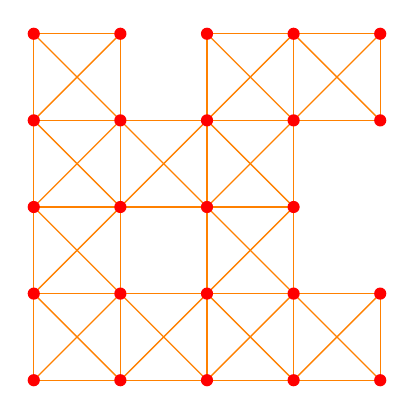
\begin{tikzpicture}[scale=1.1,line width=0.5pt]
      
      \draw[orange] (0,0) grid (4,4);
  
      \foreach \x in {0,1,2,3} {
        \foreach \y in {0,1,2,3} {
          \pgfmathparse{int(\x + 1)};
          \let\xa\pgfmathresult;
          \pgfmathparse{int(\y + 1)};
          \let\ya\pgfmathresult;
          \draw[orange] (\x,\y) -- (\xa,\ya);
        }
      }
  
      \foreach \x in {0,1,2,3} {
        \foreach \y in {1,2,3,4} {
          \pgfmathparse{int(\x + 1)};
          \let\xa\pgfmathresult;
          \pgfmathparse{int(\y - 1)};
          \let\ya\pgfmathresult;
          \draw[orange] (\x,\y) -- (\xa,\ya);
        }
      }
      
      \filldraw[color=orange,fill=white] (1,1) rectangle (2,2);
      \filldraw[color=orange,fill=white] (1,3) rectangle (2,4);
      \draw[white, ultra thick] (1,4) -- (2,4);
      \filldraw[color=orange,fill=white] (3,1) rectangle (4,3);
      \draw[white, ultra thick] (4,1) -- (4,3);
      
      \foreach \x in {0,1,2,3} {
        \foreach \y in {0,1,2,3,4} {
          \fill[red] (\x,\y) circle (2pt);
        }
      }
      \fill[red] (4,0) circle (2pt);
      \fill[red] (4,1) circle (2pt);
      \fill[red] (4,3) circle (2pt);
      \fill[red] (4,4) circle (2pt);
     
    \end{tikzpicture}
    \caption[Map]{Grid-based graph $G_{g}(M)$}
    %\label{fig:sfig1}
  \end{subfigure}
  %
  \begin{subfigure}{.5\textwidth}
    \centering
    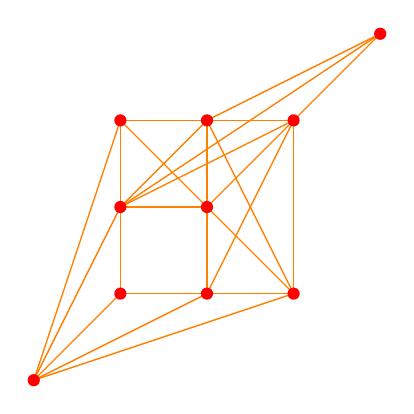
\begin{tikzpicture}[scale=1.1,line width=0.5pt]

     \draw[orange] (0,0) -- (1,1);
     \draw[orange] (0,0) -- (1,2);
     \draw[orange] (0,0) -- (1,3);
     \draw[orange] (0,0) -- (2,1);
     \draw[orange] (0,0) -- (3,1);
     
     \draw[orange] (1,1) -- (1,3);
     \draw[orange] (1,1) -- (3,1);
     
     \draw[orange] (1,2) -- (2,2);
     \draw[orange] (1,2) -- (2,3);
     \draw[orange] (1,2) -- (3,3);
     \draw[orange] (1,2) -- (4,4);
     
     \draw[orange] (1,3) -- (3,3);
     \draw[orange] (1,3) -- (3,1);
     
     \draw[orange] (2,1) -- (2,3);
     \draw[orange] (2,1) -- (3,3);
     
     \draw[orange] (2,2) -- (4,4);
     
     \draw[orange] (3,1) -- (3,3);
     \draw[orange] (3,1) -- (2,3);
     
     \draw[orange] (2,3) -- (4,4);
     
     \fill[red] (0,0) circle (2pt);
     \fill[red] (1,1) circle (2pt);
     \fill[red] (1,2) circle (2pt);
     \fill[red] (1,3) circle (2pt);
     \fill[red] (2,1) circle (2pt);
     \fill[red] (2,2) circle (2pt);
     \fill[red] (2,3) circle (2pt);
     \fill[red] (3,1) circle (2pt);
     \fill[red] (3,3) circle (2pt);
     \fill[red] (4,4) circle (2pt);
     

    \end{tikzpicture}
    \caption{Visibility graph $G_{v}(M)$}
    %\label{fig:sfi2}
  \end{subfigure}
  \caption[Graph representations of map $M$]{Graph representations of map $M$, where $n_{start} = (0,0)$ and $n_{goal} = (4,4)$}
  %\label{fig:fig}
\end{figure}

\noindent{\bfseries Lattice}\\
\noindent
The concept of a lattice is introduced because lattices are used in the upcoming explanation of discretisation, to conceptually explain how a graph is created such that it represents a specific map. A lattice $L(N)$ is a graph of $N \times N$ nodes where $N \in\mathbb{Z}$ and $N > 0$, and can be thought of as a graph that represents a map with no blocked cells. There are two types of lattice:\\

\begin{enumerate}
\item{\bfseries Octile lattice $L_{O}(N)$} --- the nodes of the lattice are arranged in a square grid, and each node is connected by an edge to the closest node, if any exists, at a bearing of any integer multiple of $\frac{\pi}{4}$ radians.

\item{\bfseries Full lattice $L_{F}(N)$} --- the nodes of the lattice are arranged in a square grid, and each node is connected by an edge to every other node in the lattice.
\end{enumerate}

\begin{figure}
  \begin{subfigure}{.5\textwidth}
    \centering
    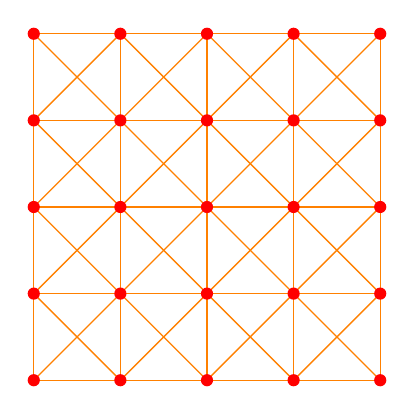
\begin{tikzpicture}[scale=1.1,line width=0.5pt]
      
      \draw[orange] (0,0) grid (4,4);
  
      \foreach \x in {0,1,2,3} {
        \foreach \y in {0,1,2,3} {
          \pgfmathparse{int(\x + 1)};
          \let\xa\pgfmathresult;
          \pgfmathparse{int(\y + 1)};
          \let\ya\pgfmathresult;
          \draw[orange] (\x,\y) -- (\xa,\ya);
        }
      }
  
      \foreach \x in {0,1,2,3} {
        \foreach \y in {1,2,3,4} {
          \pgfmathparse{int(\x + 1)};
          \let\xa\pgfmathresult;
          \pgfmathparse{int(\y - 1)};
          \let\ya\pgfmathresult;
          \draw[orange] (\x,\y) -- (\xa,\ya);
        }
      }
      
      \foreach \x in {0,1,2,3,4} {
        \foreach \y in {0,1,2,3,4} {
          \fill[red] (\x,\y) circle (2pt);
        }
      }
     
    \end{tikzpicture}
    \caption[Map]{Octile lattice $L_{O}(N)$}
    %\label{fig:sfig1}
  \end{subfigure}
  %
  \begin{subfigure}{.5\textwidth}
    \centering
    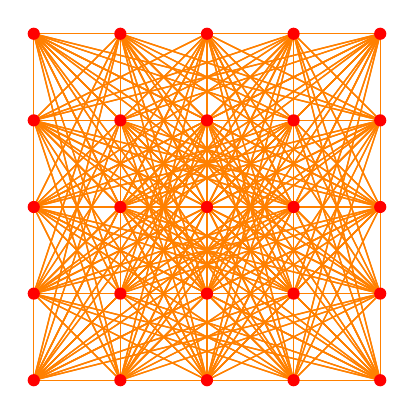
\begin{tikzpicture}[scale=1.1,line width=0.5pt]
      
      \draw[orange] (0,0) grid (4,4);
      
       \foreach \x in {0,1,2,3,4} {
        \foreach \y in {0,1,2,3,4} {
          \foreach \a in {0,1,2,3,4} {
            \foreach \b in {0,1,2,3,4} {
              \draw[orange] (\x,\y) -- (\a,\b);
            }
          }
        }
      }
      
            \foreach \x in {0,1,2,3,4} {
        \foreach \y in {0,1,2,3,4} {
          \fill[red] (\x,\y) circle (2pt);
        }
      }

    \end{tikzpicture}
    \caption{Full lattice $L_{F}(N)$}
    %\label{fig:sfi2}
  \end{subfigure}
  \caption{Octile lattice and full lattice of size $4^{2}$}
  %\label{fig:fig}
\end{figure}

\noindent{\bfseries Discretisation}\\
\noindent
Discretisation is the process of creating a graph $G(M)=(V,E)$ that represents a map $M$. The process can be visualised as refining a lattice by removing edges and nodes until the desired graph remains. A node $n$ is removed if the map indicates that $n$ represents an invalid location, and an edge $(n,n')$ is removed if there is no line of sight on the map between the locations represented by $n$ and $n'$. There are two forms of discretisation:
\begin{enumerate}
\item $d_{G}(L_{O},M) \rightarrow G_{g}(M)$ --- an octile lattice is refined to produce a grid-based graph $G_{g}$;
\item  $d_{V}(L_{O},M) \rightarrow G_{v}(M)$ --- a full lattice is refined to produce a a visibility graph $G_{v}$.
\end{enumerate}
 
\noindent
A full conceptual explanation of discretisation is provided in A.1, and the implementation of discretisation is detailed in section 3.1.2.

\subsection{The any-angle pathfinding problem}

The problem is to compute optimal or near-optimal paths, if they exist, between a given $start$ and $goal$ location in a map, by using a grid-based graph.\\

\noindent
A path $P_{M}$ through map $M$ is optimal, denoted as $P^{*}_{M}$, if there do not exist any paths through $M$ from $start$ to $goal$ with a shorter path length and a smaller path angle-sum, where:

\begin{description}
\item{\bfseries Path length}\\
The sum of the Euclidean distances between each pair of coordinates $(x_{i},y_{i})$ and $(x_{i+1},y_{i+1})$ in $P_{M}$.
\item{\bfseries Path angle-sum}\\
The sum of the (smaller) angles between each pair of path segments $(x_{i},y_{i})$ to $(x_{i+1},y_{i+1})$ and $(x_{i+1},y_{i+1})$ to $(x_{i+2},y_{i+2})$ in $P_{M}$. This is given by the scalar product between the two path segments.
\end{description}

\begin{figure}
   \centering
    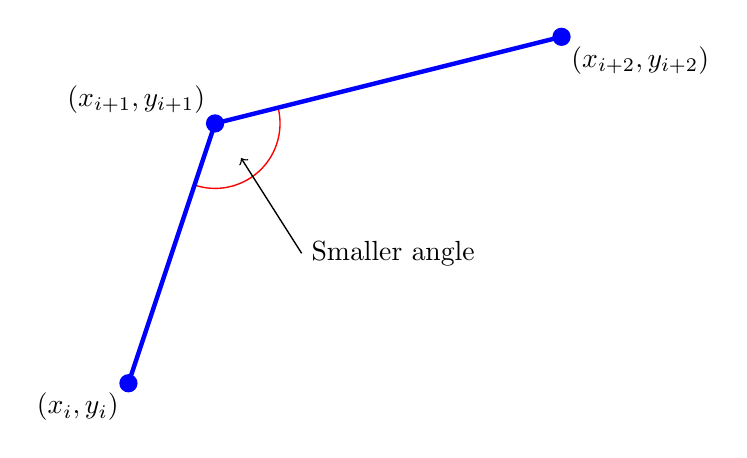
\begin{tikzpicture}[scale=1.1,line width=0.5pt]
      
     \fill[blue] (0,0) circle (3pt);
     \node[below left] at (0,0) {$(x_{i},y_{i})$};
     \fill[blue] (1,3) circle (3pt);
     \node[above left] at (1,3) {$(x_{i+1},y_{i+1})$};
     \fill[blue] (5,4) circle (3pt);
     \node[below right] at (5,4) {$(x_{i+2},y_{i+2})$};
     
     \draw[red] (1,3) ++(-108.4:0.75) arc (-108.41:14:0.75);
     %\draw[red] (1,3) circle (0.75);
     
     \draw[blue,ultra thick] (0,0) -- (1,3) -- (5,4);
     
     \node[right] at (2,1.5) {Smaller angle};
     \draw[->] (2,1.5) -- (1.3,2.6);
     
    \end{tikzpicture}
    \caption{Smaller angle between a pair of path segments}
    %\label{fig:sfig1}
  \end{figure}


\subsection{Solving the any-angle pathfinding problem}

\noindent
The steps required to find an optimal or near-optimal path $P_{M}$ through a map $M$ from $start$ to $goal$, as introduced in subsection 2.1.2, will now be re-stated using the notation that has been introduced in this chapter:
\begin{enumerate}
\item a grid-based graph $G_{g}(M)$ that represents the map $M$ is produced, where each node in the graph represents a location in the map; 
\item a pathfinding algorithm\footnote{{\em Block A*} operates in a different way, and is dealt with separately.} is applied to the $G_{g}(M)$, which returns a path $P_{G_{g}(M)} = (n_{start},n_{1},...,n_{goal})$;
\item $P_{G_{g}(M)}$ corresponds to the path $P_{M} = (x_{start},x_{1},...,x_{goal})$, using the correspondence that $x_{i}$ is the location in map $M$ that is represented by the node $n_{i}$ of graph $G_{g}(M)$.
\end{enumerate}

\noindent
The only step that remains to be introduced is step 2 which involves the application of a pathfinding algorithm to a graph as covered in section 2.2.

\section{Any-angle pathfinding algorithms}

\noindent
This section starts with an introduction of pathfinding over graphs, followed by definitions of the two types of pathfinding algorithms: `classic' and `any-angle'. Classic pathfinding algorithms are presented first as they explain some of the important concepts required to understand the more complicated any-angle algorithms the constitute the core of this dissertation, and to serve as a useful benchmark for comparison in the {\bfseries Evaluation} chapter. The remainder of the section describes the pathfinding algorithms in detail.
 
\subsection{Pathfinding over graphs}

When applied to a graph $G(M)$, a pathfinding algorithm returns a path $P_{G(M)}$ between a given $n_{start}$ and $n_{goal}$.\\

\noindent
Section 2.1.3 introduced the concept of a graph $G(M)$ that is a representation of a map $M$ such that each node $n$ in $G(M)$ has an associated coordinate $coord$. In addition, all of the algorithms require graph nodes to have the following two parameters:
\begin{itemize}
\item {\em g-value} --- the path length of the shortest path between $n_{start}$ and $n$ that the algorithm has found thus far;
\item {\em parent} --- a pointer to the previous node in the shortest path between $n_{start}$ and $n$ that the algorithm has found thus far. Therefore, the shortest path between $n_{start}$ and $n$ is found by recursively following the $parent$ pointers from $n$ to $n_{start}$.
\end{itemize}

\noindent
At the start of the algorithm $n.g = \infty$ and $n.parent = \bot$ for all nodes (since the algorithm hasn't found any paths between any nodes at this point)\footnote{Where $\bot$ denotes that the parameter value is undefined.}. On termination, if a path exists then $n_{goal}.g$ is the path length of the shortest path found by the algorithm from $n_{start}$ to $n_{goal}$, and this path is found by recursively following the $parent$ pointers from $n_{goal}$ to $n_{start}$\footnote{The pathfinding algorithm guarantees $n_{start}.parent = \bot$.}; if a path doesn't exist then $n_{goal} = \bot$.

\subsection {Types of pathfinding algorithms}

A summary of our findings so far motivates the need for a more advanced type of pathfinding algorithm than the classic pathfinding algorithms. As seen in the {\bfseries Introduction}, even when a path through a grid-based graph $G_{g}(M)$ is optimal, the corresponding path through the map $M$ may not be. Since classic pathfinding algorithms find optimal paths through graphs, and because the decision has been made to use grid-based graphs, it is clear that using classic pathfinding algorithms will give sub-optimal paths through maps.\\

\noindent
Any-angle pathfinding algorithms aim to improve upon classic pathfinding algorithms by taking a grid-based graph $G_{g}(M)$ and selectively adding a small amount of edges to $G_{g}(M)$ (i.e. `augmenting' $G_{g}(M)$) so that it closely resembles a visibility graph in the region that surrounds the path. In this way, any-angle pathfinding algorithms aim to benefit from the efficiency of grid-based graphs and the optimality of visibility graphs, though tradeoffs are required on both sides. These explanations are now formalised:

\begin{description}
\item{\bfseries Classic pathfinding algorithm}\\ 
A classic pathfinding algorithm will return the optimal\footnote{The definition of an optimal path $P_{G_{M}}$ through a graph is analogous to the definition of a an optimal path $P_{M}$ in subsection 2.1.3.}  path $P^{*}_{G(M)}$ through $G(M)$.\footnote{Remember: $P_{G(M)}$ corresponds to $P_{M}$, but the optimal path $P^{*}_{G(M)}$ through $G(M)$ does not necessarily correspond to the optimal path $P^{*}_{M}$ through $M$ --- this idea was illustrated in the {\bfseries Introduction} chapter.}
\item{\bfseries Any-angle pathfinding algorithm}\\
An any-angle pathfinding algorithm will return the optimal path $P^{*}_{G'(M)}$ through $G'(M)$, where the augmented graph $G'(M)$ may have extra edges to $G(M)$.
\end{description}

\subsection {Dijkstra's shortest paths}

Most of the algorithms in this dissertation are derivatives of the {\em A*} graph traversal algorithm, which itself is a derivative of {\em Dijkstra}'s famous shortest-path algorithm.\\

\noindent{\bfseries Overview}\\
\noindent
Starting at $n_{start}$, {\em Dijkstra} selects and then processes (or `expands') one node at a time (see subsection {\bfseries Expansion}). It is a provable\cite{CormenDijkstra} invariant of the algorithm that when a node $n$ is selected to be processed, $n.g$ is equal to the length of the shortest path in the graph to $n$ from $n_{start}$. For this reason, once a node has been expanded, it need not be expanded again (this would incur unnecessary work)\footnote{A set $closedSet$ ensures that this does not occur.}. When $n_{goal}$ is expanded, $n_{goal}.g$ is the length of the shortest path in $G$ from $n_{start}$ to $n_{goal}$ (according to the invariant condition), so the algorithm terminates.\\

\noindent{\bfseries Expansion}\\
\noindent
{\em Dijkstra} selects the next node $n$ to expand from $openSet$, a priority queue\footnote{The set and priority queue methods $add()$, $pop()$ and  $contains()$ are defined in the usual way.} that stores nodes in increasing order of their {\em g-values}. To expand $n$: for each $n_{neigh}$ of the neighbours of $n$, {\em Dijkstra} attempts to `relax' $n_{neigh}$ --- that is to say: {\em Dijkstra} tests whether the shortest path to $n_{neigh}$ that it had found so far (as defined by the $parent$ pointers from $n$ to $n_{start}$) is longer than the path to $n_{neigh}$ that is made up of the shortest path found so far to $n$ and then from $n$ to $n_{neigh}$\footnote{This condition relies on the provable\cite{CormenDijkstra} fact that any sub-path of a shortest path is itself a shortest path.}, which can be stated as the condition:
\begin{equation}
n.g + (n,n_{neigh}).weight < n_{neigh}.g
\end{equation}
\noindent
and if (2.1) is true, {\em Dijkstra} updates $n_{neigh}$ to reflect that the newly discovered shortest path to it is the one that goes via $n$, by: 
\begin{itemize}
\item updating the $parent$ of $n_{neigh}$ to $n$;
\item updating the {\em g-value} of $n_{neigh}$ to $n.g + (n,n_{neigh}).weight$ .
\end{itemize}
Finally, $n_{neigh}$ is added to $openSet$ if it is not already in it, and then the next node to be expanded is selected.\\

\noindent{\bfseries Termination}\\
\noindent
This process continues until $openSet$ is empty or $n_{goal}$ has been processed, at which point the algorithm terminates. If a valid path exists, {\em Dijkstra} returns $P^{*}_{G}$. Otherwise it returns $\bot$.\

\begin{algorithm}
  \SetAlgoLined\DontPrintSemicolon
  \SetKwFunction{dijkstra}{Dijkstra}\SetKwFunction{update}{Update}
  \SetKwProg{myDef}{def}{}{}
  \myDef{\dijkstra{G, $n_{start}$, $n_{goal}$}}{
  \nl $openSet \gets \bot$\;
  \nl $closedSet \gets \bot$\;
  \nl $n_{start}.g \gets 0$\;
  \nl $openSet.add(n_{start})$\;
  \nl \While{$openSet \neq \bot$} {
    \nl $n_{curr} \gets openSet.pop()$\;
    \nl $closedSet.add(n_{curr})$\;
    \nl \If{$n_{curr} = n_{goal}$} {
      \nl \KwRet{$n_{goal}$}\;
    }
    \nl \ForEach{$n_{neigh}$ of $n_{curr} $} {
      \nl \If{$closedSet.contains(n_{neigh}) = false $} {
        \nl \If{$\update(n_{neigh}) = true$} {
          \nl \If{$openSet.contains(n_{neigh}) = false $} {
            \nl $openSet.add(n_{neigh})$\;
          }
        }
      }
    }
  }
  \nl \KwRet{$\bot$}\;
}{}
  \setcounter{AlgoLine}{0}
  \myDef{\update{$n_{neigh}$}}{
    \nl \uIf{$n_{curr}.g + (n_{curr},n_{neigh}).weight < n_{neigh}.g$} {
      \nl $n_{neigh}.g = n_{curr}.g + (n_{curr},n_{neigh}).weight$\;
      \nl $n_{neigh}.parent = n_{curr}$\;
      \nl \KwRet{$true$}\;
    } \nl \Else {
      \nl \KwRet{$false$}\;
    } 
  }
  \caption{{\sc Dijkstra}}
\end{algorithm} 

\subsection {A*}

{\em A*} is based on {\em Dijkstra's shortest-paths} algorithm and also finds the optimal path\cite{Hart68} $P^{*}_{G}$ through a graph $G$, but uses a heuristic $h$ to reduce the number of node expansions required.\\

\noindent
In addition to a {\em g-value} and a {\em parent}, each node also has a:
\begin{itemize}
\item {\em h-value} --- Euclidean distance between {$n$} and {$n_{goal}$}: a cheaply computable monotonic estimate\footnote{The monotonicity of Euclidean distance as a heuristic ensures that {\em A*}, like {\em Dijkstra}, is complete (if a path exists, it finds it) and optimal (if a path is found, it is a shortest distance path)} of the actual shortest path length between $n$ and $n_{goal}$.
\end{itemize}

\noindent
While {\em Dijkstra} preferentially expands nodes with low {\em g-value}s (by utilising a priority queue called {\em openSet}, which sorts using {\em g-values}), {\em A*} preferentially expands nodes with low {\em f-score}s (by utilising a priority queue called {\em openSet}, which sorts using {\em f-values}), where a node $n$'s {\em f-score} is the algorithm's current estimate of the shortest path from $n_{start}$ via $n$ to $n_{goal}$ --- that is to say:
\begin{equation}
n.f = n.g + n.h
\end{equation}

\noindent
The pseudo-code for {\em A*} differs only from {\em Dijkstra} in the {\tt Update} subroutine, where the {\em h-score} must also be set.

\begin{algorithm}
  \SetAlgoLined\DontPrintSemicolon
  \SetKwFunction{update}{Update}
  \SetKwProg{myDef}{def}{}{}
  \myDef{\update{$n_{neigh}$}}{
    \nl \uIf{$n_{curr}.g + (n_{curr},n_{neigh}).weight < n_{neigh}.g$} {
      \nl $n_{neigh}.g \gets n_{curr}.g + euclidean(n_{curr},n_{neigh})$\;
      \nl $n_{neigh}.h \gets euclidean(n_{neigh},n_{goal})$\;
      \nl $n_{neigh}.parent = n_{curr}$\;
      \nl \KwRet{$true$}\;
    } \nl \Else {
      \nl \KwRet{$false$}\;
    } 
  }
  \caption{{\tt Update} from {\sc A*}}
\end{algorithm} 

\subsection {A* with post-smoothing}

{\em A* with post-smoothing} is the first any-angle pathfinding algorithm that is introduced in this project. It applies a post-processing step to the path $(n_{start}, n_{1}, \ldots, n_{goal})$ returned by {\em A*}, which `smoothes'  and therefore shortens this path.\\

\noindent The smoothing is achieved by changing the $parent$ pointer for some nodes in the original path. For example, the $parent$ of a node $n_{j}$ in the original path is defined as $n_{j-1}$, but {\em A* with post-smoothing} may change $n_{j}.parent$ so that is points to a different node in the original path (call it $n_{i}$) that is closer to the $start$ of the path than $n_{j-1}$ (i.e. $i<j-1$) --- this re-parenting is only allowed if there is a line of sight between $n_{j}$ and $n_{i}$. If $G(M)$ did not have an edge between $n_{j}$ and $n_{i}$, then this re-parenting procedure has the effecting of augmenting $G(M)$ by adding an edge to it.\\

\begin{figure}
  \begin{subfigure}{.3\textwidth}
    \centering
    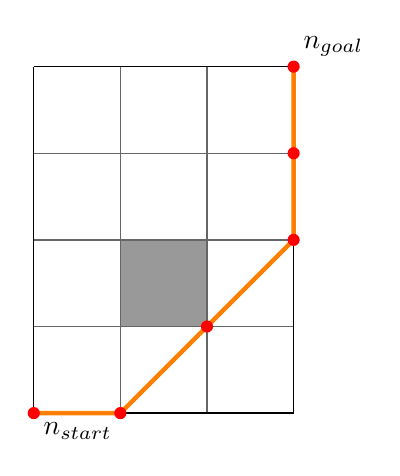
\begin{tikzpicture}[scale=1.1,line width=0.5pt]
    
      \draw[color=black!60] (0,0) grid (3,4);
    
      \node[below right] at (0,0) {$n_{start}$};
      \node[above right] at (3,4) {$n_{goal}$};

      \filldraw[color=black!60,fill=black!40] (1,1) rectangle (2,2); 
      \draw (0,0) -- (0,4);
      \draw (0,0) -- (3,0);
      \draw (3,4) -- (0,4);
      \draw (3,4) -- (3,0);
    
      \draw[orange, ultra thick] (0,0) -- (1,0) -- (3,2) -- (3,4);
      \fill[red] (0,0) circle (2pt);
      \fill[red] (1,0) circle (2pt);
      \fill[red] (2,1) circle (2pt);
      \fill[red] (3,2) circle (2pt);
      \fill[red] (3,3) circle (2pt);
      \fill[red] (3,4) circle (2pt);

    \end{tikzpicture}
    \caption{Original path}
    %\label{fig:sfi2}
  \end{subfigure}
  \begin{subfigure}{.3\textwidth}
    \centering
    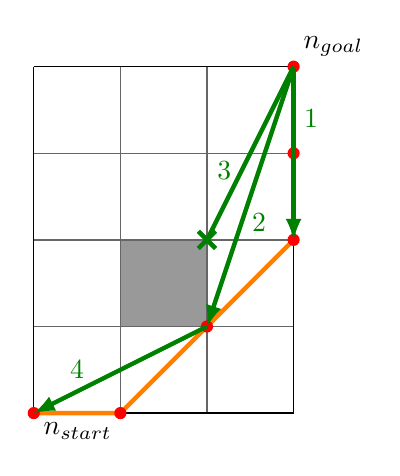
\begin{tikzpicture}[scale=1.1,line width=0.5pt]
    
      \draw[color=black!60] (0,0) grid (3,4);
    
      \node[below right] at (0,0) {$n_{start}$};
      \node[above right] at (3,4) {$n_{goal}$};

      \filldraw[color=black!60,fill=black!40] (1,1) rectangle (2,2); 
      \draw (0,0) -- (0,4);
      \draw (0,0) -- (3,0);
      \draw (3,4) -- (0,4);
      \draw (3,4) -- (3,0);
      
      \draw[orange, ultra thick] (0,0) -- (1,0) -- (3,2) -- (3,4);
      \fill[red] (0,0) circle (2pt);
      \fill[red] (1,0) circle (2pt);
      \fill[red] (2,1) circle (2pt);
      \fill[red] (3,2) circle (2pt);
      \fill[red] (3,3) circle (2pt);
      \fill[red] (3,4) circle (2pt);
      
      \draw[green!50!black, ultra thick,>=latex,->] (3,4) -- (3,2);
      \draw[green!50!black, ultra thick,>=latex,->] (3,4) -- (2,1);
      \draw[green!50!black, ultra thick] (3,4) -- (2,2);
      \draw[green!50!black,ultra thick] (1.9,2.1) -- (2.1,1.9);
      \draw[green!50!black,ultra thick] (1.9,1.9) -- (2.1,2.1);
      \draw[green!50!black, ultra thick, >=latex,->] (2,1) -- (0,0);
      
      \node[green!50!black] at (3.2,3.4) {1};
      \node[green!50!black] at (2.6,2.2) {2};
      \node[green!50!black] at (2.2,2.8) {3};
      \node[green!50!black] at (0.5,0.5) {4};


    \end{tikzpicture}
    \caption{Line of sight tests} \label{fig:astarsmoothed}
  \end{subfigure}
  %
  \begin{subfigure}{.3\textwidth}
    \centering
    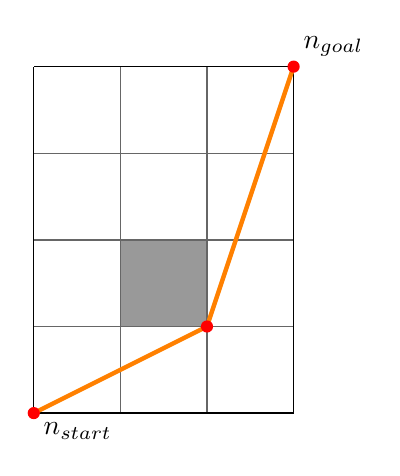
\begin{tikzpicture}[scale=1.1,line width=0.5pt]
    
      \draw[color=black!60] (0,0) grid (3,4);
    
      \node[below right] at (0,0) {$n_{start}$};
      \node[above right] at (3,4) {$n_{goal}$};

      \filldraw[color=black!60,fill=black!40] (1,1) rectangle (2,2); 
      \draw (0,0) -- (0,4);
      \draw (0,0) -- (3,0);
      \draw (3,4) -- (0,4);
      \draw (3,4) -- (3,0);
    
      \draw[orange, ultra thick] (0,0) -- (2,1) -- (3,4);
      \fill[red] (0,0) circle (2pt);
      \fill[red] (2,1) circle (2pt);
      \fill[red] (3,4) circle (2pt);

    \end{tikzpicture}
    \caption{Improved path}
    %\label{fig:sfi2}
  \end{subfigure}
  \caption{{\em A* with post-smoothing}}
  %\label{fig:fig}
\end{figure}


\begin{algorithm}
  \SetAlgoLined\DontPrintSemicolon
  \SetKwFunction{ps}{PostSmoothing}\SetKwFunction{los}{LineOfSight}
  \SetKwProg{myDef}{def}{}{}
  \myDef{\ps{$n_{start}, n_{goal}$}}{
    \nl $n_{curr} \gets n_{goal} $\;
    \nl $n_{next} \gets n_{goal}.parent.parent $\;
    \nl \uIf {$n_{next}  = \bot$} {
      \nl \KwRet{} \;
    }
    \nl \While{$true$} {
      \nl \While{$\los(n_{curr} ,n_{next} )$} {
        \nl $n_{curr}.parent \gets n_{next} $\;
        \nl $n_{next}  \gets n_{next} .parent$\;
        \nl \uIf{$n_{next}  = n_{start}$} {
          \nl \KwRet{} \;
        }
      }
      \nl $n_{curr}  \gets n_{next} $\;
      \nl \uIf{$n_{curr}.parent = n_{start}$} {
        \nl \KwRet{}\;
        }
      \nl $n_{next}  \gets n_{next}.parent.parent$\;
    }
  }
  \caption{{\tt PostSmoothing} from {\sc A* with post-smoothing}}
\end{algorithm} 

\subsection {Theta*}

The previous subsection demonstrated how {\em A* with post-smoothing} performs smoothing on the path returned by the classic pathfinding algorithm {\em A*}. In contrast, {\em Theta*} smoothes as it goes along by progressing in a similar way to {\em A*}, by also attempting to re-parent each of $n_{curr}$'s neighbours $n_{neigh}$ with $n_{curr}.parent$ at the time when $n_{curr}$ is expanded\footnote{As with {\em A* with post-smoothing}, re-parenting in {\em Theta*} occurs if a line of sight exists between the coordinates represented by the two nodes in question.}.\\

\noindent
The pseudo-code for {\em Theta*} differs only from {\em A*} in the {\tt Update} subroutine.

\begin{algorithm}
  \SetAlgoLined\DontPrintSemicolon
  \SetKwFunction{update}{Update}\SetKwFunction{los}{LineOfSight}
  \SetKwProg{myDef}{def}{}{}
  \myDef{\update{$n_{neigh}$}}{
    \nl \uIf{$\los(n_{neigh}, n_{curr}.parent) = true$} {
      \nl \uIf{$n_{curr}.parent.g + (n_{curr}.parent,n_{neigh}).weight < n_{neigh}.g$} {
        \nl $n_{neigh}.g \gets n_{neigh}.parent.g + (n_{curr}.parent,n_{neigh}).weight$\;
        \nl $n_{neigh}.f \gets euclidean(n_{neigh},n_{goal})$\;
        \nl $n_{neigh}.parent \gets n_{curr}.parent$\;
        \nl \KwRet{$true$}\;
      } \nl \Else {
        \nl \KwRet{$false$}\;
      } 
    } \nl \Else {
      \nl \uIf{$n_{curr}.g + (n_{curr},n_{neigh}).weight < n_{neigh}.g$} {
        \nl $n_{neigh}.g \gets n_{curr}.g + (n_{curr},n_{neigh}).weight$\;
        \nl $n_{neigh}.f \gets euclidean(n_{neigh},n_{goal})$\;
        \nl $n_{neigh}.parent \gets n_{curr}$\;
        \nl \KwRet{$true$}\;
      } \nl \Else {
        \nl \KwRet{$false$}\;
      } 
    }
  }
  \caption{{\tt Update} from {\sc Theta*}}
\end{algorithm} 

\subsection {Lazy Theta*}

{\em Lazy Theta*} attempts to refine {\em Theta*} by finding similar paths despite performing fewer line of sight tests.\\

\noindent
While {\em Theta*} performs a line of sight test for every neighbour $n_{neigh}$ of every node $n_{curr}$ that is expanded, {\em Lazy Theta*} only performs line of sight tests for every node $n_{curr}$ that is expanded --- by initially assuming that all line of sight tests pass, and only actually doing a test between a node and its parent when the node is expanded. Whenever a line of sight test fails, a costly cleanup step is required to undo the effect of an incorrect assumption.\\

\noindent
The paths returned by {\em Lazy Theta*} are not always the same as those returned by {\em Theta*} since the edge relaxation occurs at a different point in the iteration.\\

\begin{algorithm}
  \SetAlgoLined\DontPrintSemicolon
  \SetKwFunction{dijkstra}{LazyTheta*}\SetKwFunction{update}{Update}\SetKwFunction{los}{LineOfSight}\SetKwFunction{init}{Initialise}
  \SetKwProg{myDef}{def}{}{}
  
  \myDef{\dijkstra{G, $n_{start}$, $n_{goal}$}}{
  \nl $openSet \gets \bot$\;
  \nl $closedSet \gets \bot$\;
  \nl $n_{start}.g \gets 0$\;
  \nl $openSet.add(n_{start})$\;
  \nl \While{$openSet \neq \bot$} {
    \nl $n_{curr} \gets openSet.pop()$\;
    \nl $\init(n_{curr})$\;
    \nl $closedSet.add(n_{curr})$\;
    \nl \If{$n_{curr} = n_{goal}$} {
      \nl \KwRet{$n_{goal}$}\;
    }
    \nl \ForEach{$n_{neigh}$ of $n_{curr} $} {
      \nl \If{$closedSet.contains(n_{neigh}) = false $} {
        \nl \If{$\update(n_{neigh}) = true$} {
          \nl \If{$openSet.contains(n_{neigh}) = false $} {
            \nl $openSet.add(n_{neigh})$\;
          }
        }
      }
    }
  }
  \nl \KwRet{$\bot$}\;
}{}

  \myDef{\init{$n_{curr}$}}{
      \nl \uIf{$\los(n_{curr}, n_{curr}.parent) = false$} {
      \tcp{cleanup code if line of sight doesn't pass}
        \nl $newParent \gets \argmin\limits_{n' \in expandedNeigh(n_{curr})} (n'.g + (n',n_{curr}).weight)$\;
        \nl $n_{curr}.parent \gets n'$\;
        \nl $n_{curr}.g \gets n'.g + (n',n_{curr}).weight$\;
       } 
  }
  \myDef{\update{$n_{neigh}$}}{
        \tcp{assume line of sight test passes}
      \nl \uIf{$n_{curr}.parent.g + (n_{curr}.parent,n_{neigh}).weight < n_{neigh}.g$} {
        \nl $n_{neigh}.g \gets n_{neigh}.parent.g + (n_{curr}.parent,n_{neigh}).weight$\;
        \nl $n_{neigh}.f \gets euclidean(n_{neigh},n_{goal})$\;
        \nl $n_{neigh}.parent \gets n_{curr}.parent$\;
        \nl \KwRet{$true$}\;
      } \nl \Else {
        \nl \KwRet{$false$}\;
      } 
  }
  \caption{{\sc Lazy Theta*}}
\end{algorithm} 

\subsection {Block A*}

\noindent
{\em Block A*} is the most complex algorithm in this dissertation. It was published in 2011, and is at the very cutting edge of any-angle path-finding algorithmic research.\\

\noindent{\bfseries Overview}\\
\noindent
{\em Block A*} aims to achieve faster computation of paths by doing far fewer expansions than the algorithms that have already been introduced, because {\em Block A*} expands `blocks' rather than just nodes, where a block is a graph-like structure that represents an entire sub-area of the overall map $M$ --- hence each expansion in {\em Block A*} makes far more progress than an expansion in the other algorithms. However, the expansion of a block is more complicated than that of a node as it requires obtaining the values of the shortest paths between points that lie on different sides of a block --- though this extra complexity is partly assuaged by the fact that these paths do not need to be explicitly calculated since they are available from a precalculated {\em Local Distance Database (LDDB)}.\\

\noindent
The remainder of this subsection contains a novel explanation of {\em Block A*} which draws close parallels with the graph-based explanations provided in the previous sections for {\em Dijkstra} and {\em A*}. Due to the complexity of {\em Block A*}, this explanation is mathematically and notationally intensive, yet considerably more succinct that the example based-explanation found in {\em Yap et at.}'s original paper\cite{Yap11}.\\

\noindent{\bfseries Blocks}\\
\noindent
A block $B_{i,j}$ of size ${N_{B}}^{2}$ is a graph-like structure that represents the area of the map $M$ covered by all cells $C_{k,l} \in M$ where $i \leq k \leq i+N_{B}$ and $j \leq l \leq j+N_{B}$.\\

\noindent
For each block $B_{i,j} = (V_{i,j},E_{i,j})$, node $n \in V_{i,j}$ represents a location $(a,b) \in M$ where $(a,b)$ lies on the boundary of $B_{i,j}$ --- that is to say, where $a=i$ or $a=i+N_{B}$, and $b=j$ or $b=j+N_{B}$. $n$ has a $g-value$, $h-value$ and $parent$ defined as per {\em A*}.\footnote{Except when the block is $B_{goal}$, when the {\em h-value} is the length of the shortest path between $n$ and $n_{goal}$ --- this is discussed in the {\em Initialisation} step of the algorithm.}\\

\noindent
If the locations represented by $B_{i,j}$ contain the location $start$ or $goal$ then $B_{i,j}$ is called $B_{start}$ or $B_{goal}$ respectively, and $B_{i,j}$ has an extra node $n_{start}$ or $n_{goal}$ with edges from that node to every other node in the block. For all other blocks, called `regular' blocks, there is an edge between every pair of nodes in $B_{i,j}$.\\

\begin{figure}
    \centering
    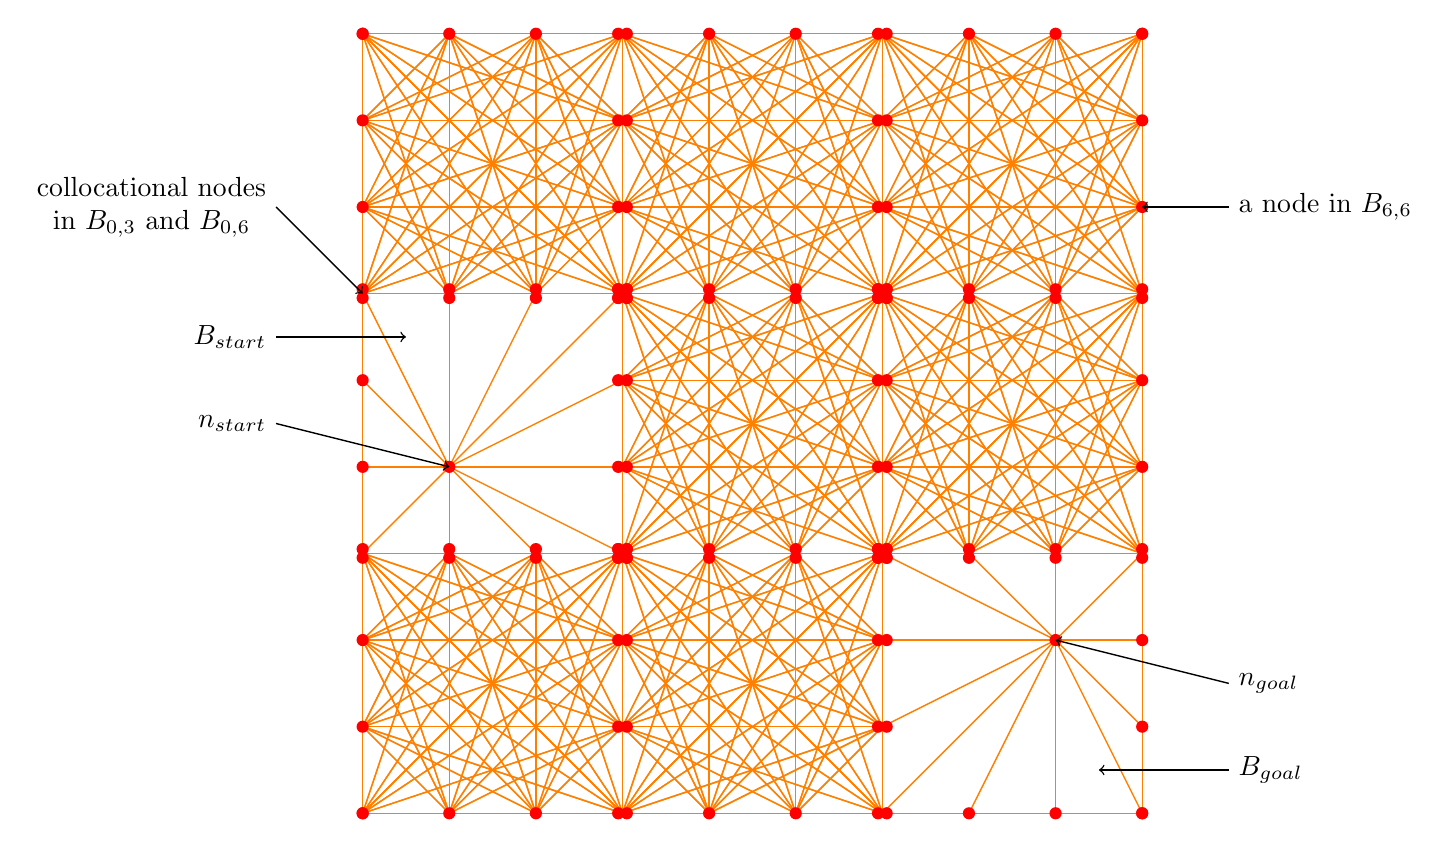
\begin{tikzpicture}[scale=1.1,line width=0.5pt]
  
      \foreach \i in {0,3,6} {
      \foreach \j in {0,3,6} {
      \foreach \x in {0,1,2,3} {
        \foreach \y in {0,3} {
          \foreach \a in {0,1,2,3} {
            \foreach \b in {0,3} {
             \pgfmathparse{int(\x + \i)};
             \let\xn\pgfmathresult;
             \pgfmathparse{int(\a + \i)};
             \let\an\pgfmathresult;
             \pgfmathparse{int(\y + \j)};
             \let\yn\pgfmathresult;
             \pgfmathparse{int(\b + \j)};
             \let\bn\pgfmathresult;
              \draw[orange] (\xn,\yn) -- (\an,\bn);
              \draw[orange] (\yn,\xn) -- (\bn,\an);
            }
          }
        }
      }
      }}
      
      \foreach \i in {0,3,6} {
      \foreach \j in {0,3,6} {
      \foreach \x in {1,2} {
        \foreach \y in {0,3} {
          \foreach \a in {1,2} {
            \foreach \b in {0,3} {
             \pgfmathparse{int(\x+\i)};
             \let\xn\pgfmathresult;
             \pgfmathparse{int(\a+\j)};
             \let\an\pgfmathresult;
             \pgfmathparse{int(\y+\j)};
             \let\yn\pgfmathresult;
             \pgfmathparse{int(\b+\i)};
             \let\bn\pgfmathresult;
              \draw[orange] (\xn,\yn) -- (\bn,\an);
              \draw[orange] (\yn,\xn) -- (\an,\bn);
            }
          }
        }
      }
      }}
      
      \filldraw[color=orange, fill=white] (0,3) rectangle (3,6);
      \filldraw[color=orange, fill=white] (6,0) rectangle (9,3);
      
      \draw[orange] (1,4) -- (0,3);
      \draw[orange] (1,4) -- (0,4);
      \draw[orange] (1,4) -- (0,5);
      \draw[orange] (1,4) -- (0,6);
      \draw[orange] (1,4) -- (3,3);
      \draw[orange] (1,4) -- (3,4);
      \draw[orange] (1,4) -- (3,5);
      \draw[orange] (1,4) -- (3,6);
      \draw[orange] (1,4) -- (1,3);
      \draw[orange] (1,4) -- (2,3);
      \draw[orange] (1,4) -- (1,6);
      \draw[orange] (1,4) -- (2,6);
      \fill[red] (1,4) circle (2pt);
      \draw[orange] (8,2) -- (6,0);
      \draw[orange] (8,2) -- (6,1);
      \draw[orange] (8,2) -- (6,2);
      \draw[orange] (8,2) -- (6,3);
      \draw[orange] (8,2) -- (9,0);
      \draw[orange] (8,2) -- (9,1);
      \draw[orange] (8,2) -- (9,2);
      \draw[orange] (8,2) -- (9,3);
      \draw[orange] (8,2) -- (7,0);
      \draw[orange] (8,2) -- (8,0);
      \draw[orange] (8,2) -- (7,3);
      \draw[orange] (8,2) -- (8,3);
      \fill[red] (8,2) circle (2pt);
      
      \foreach \x in {0,1,2,2.95,3.05,4,5,5.95,6.05,7,8,9} {
        \foreach \y in {0,9} {
              \fill[red] (\x,\y) circle (2pt);
              \fill[red] (\y,\x) circle (2pt);
        }
      }
      
      \foreach \x in {1,2,4,5,7,8} {
        \foreach \y in {3,6} {
          \pgfmathparse{(\y + 0.05)};
           \let\ya\pgfmathresult;
            \pgfmathparse{(\y - 0.05)};
           \let\yb\pgfmathresult;
              \fill[red] (\x,\ya) circle (2pt);
              \fill[red] (\x,\yb) circle (2pt);
              \fill[red] (\ya,\x) circle (2pt);
              \fill[red] (\yb,\x) circle (2pt);
        }
      }
      
       \foreach \x in {3,6} {
        \foreach \y in {3,6} {
          \pgfmathparse{(\x + 0.05)};
           \let\xa\pgfmathresult;
            \pgfmathparse{(\x - 0.05)};
           \let\xb\pgfmathresult;
           \pgfmathparse{(\y + 0.05)};
           \let\ya\pgfmathresult;
              \fill[red] (\xa,\ya) circle (2pt);
              \fill[red] (\xb,\ya) circle (2pt);
              \fill[red] (\ya,\xa) circle (2pt);
              \fill[red] (\ya,\xb) circle (2pt);
        }
      }
      
             \foreach \x in {3,6} {
        \foreach \y in {3,6} {
          \pgfmathparse{(\x + 0.05)};
           \let\xa\pgfmathresult;
            \pgfmathparse{(\x - 0.05)};
           \let\xb\pgfmathresult;
           \pgfmathparse{(\y - 0.05)};
           \let\ya\pgfmathresult;
              \fill[red] (\xa,\ya) circle (2pt);
              \fill[red] (\xb,\ya) circle (2pt);
              \fill[red] (\ya,\xa) circle (2pt);
              \fill[red] (\ya,\xb) circle (2pt);
        }
      }
      
      \node[left] at (-1,5.5) {$B_{start}$};
      \draw[->] (-1,5.5) -- (0.5,5.5);
      
      \node[left] at (-1,4.5) {$n_{start}$};
      \draw[->] (-1,4.5) -- (1,4);
      
      \node[right] at (10,1.5) {$n_{goal}$};
      \draw[->] (10,1.5) -- (8,2);
      
      \node[right] at (10,0.5) {$B_{goal}$};
      \draw[->] (10,0.5) -- (8.5,0.5);
      
      \node[right] at (10,7) {a node in $B_{6,6}$};
      \draw[->] (10,7) -- (9,7);
      
      \node[left,align=center] at (-1,7) {collocational nodes \\in $B_{0,3}$ and $B_{0,6}$};
      \draw[->] (-1,7) -- (0,6);
      
     
    \end{tikzpicture}
    \caption[Set of blocks]{Logical view of a map of size $9^{2}$ represented as a set of 9 blocks of size $3^{2}$}
  %\label{fig:fig}
\end{figure}

\noindent For all edges $(n,n') \in B$, {\em $(n,n').weight$ is the length of the shortest path in map $M$ between the two locations represented by $n$ and $n'$}.\footnote{This important distinction bears clarificiation: in grid-based graphs and visibility graphs, an edge denotes that an agent can travel in a straight line between the two nodes that the edge connects, whereas an edge in a block merely denotes that an agent can travel between those two nodes {\em on some path within that block}, where the length of the shortest path between the two nodes (which may not be a straight line) is the edge weight which may range from $0$ to $\infty$.} See Figure 2.8. The edge weights for regular blocks are discovered by querying the {\em Local Distance Database (LDDB)}, but the weights of edges in $B_{start}$ and $B_{goal}$ are calculated separately --- this is discussed in the {\bfseries Implementation} chapter.\\

\begin{figure}
    \centering
    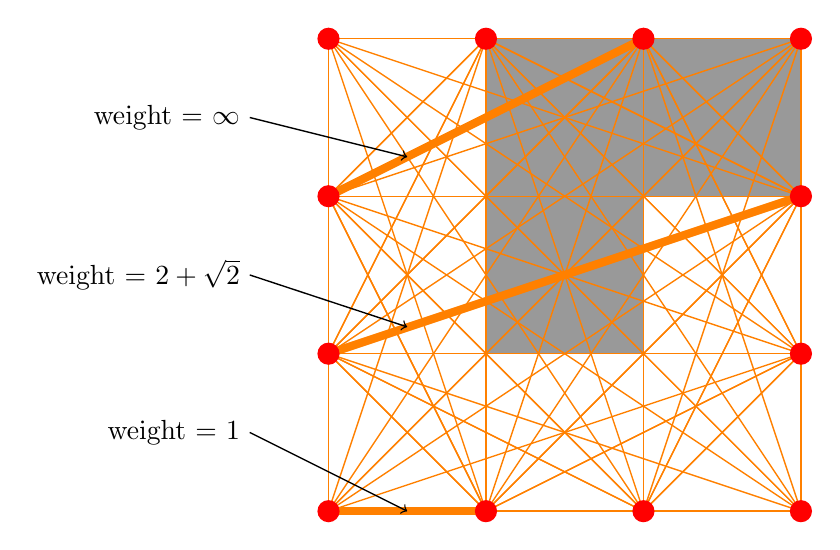
\begin{tikzpicture}[scale=2,line width=0.5pt]
    
      \filldraw[color=black!60,fill=black!40] (1,1) rectangle (2,3); 
      \filldraw[color=black!60,fill=black!40] (1,2) rectangle (3,3); 
  
      \foreach \x in {0,1,2,3} {
        \foreach \y in {0} {
          \foreach \a in {0,1,2,3} {
            \foreach \b in {3} {
              \draw[orange] (\x,\y) -- (\a,\b);
              \draw[orange] (\y,\x) -- (\b,\a);
            }
          }
        }
      }
      
      \foreach \x in {1,2} {
        \foreach \y in {0,3} {
          \foreach \a in {0,3} {
            \foreach \b in {1,2} {
              \draw[orange] (\x,\y) -- (\a,\b);
              \draw[orange] (\y,\x) -- (\b,\a);
            }
          }
        }
      }
      
      \draw[orange, line width = 3pt] (0,0) -- (1,0);
      \draw[orange, line width = 3pt](0,1) -- (3,2);
      \draw[orange, line width = 3pt] (0,2) -- (2,3);
      
      \node[left] at (-0.5,0.5) {weight = $1$};
      \draw[->] (-0.5,0.5) -- (0.5,0);
      \node[left] at (-0.5,1.5) {weight = $2 + \sqrt 2$};
      \draw[->] (-0.5,1.5) -- (0.5,1.17);
      \node[left] at (-0.5,2.5) {weight = $\infty$};
      \draw[->] (-0.5,2.5) -- (0.5,2.25);
      
      \fill[red] (0,0) circle (2pt);
      \fill[red] (0,1) circle (2pt);
      \fill[red] (0,2) circle (2pt);
      \fill[red] (0,3) circle (2pt);
      \fill[red] (3,0) circle (2pt);
      \fill[red] (3,1) circle (2pt);
      \fill[red] (3,2) circle (2pt);
      \fill[red] (3,3) circle (2pt);
      \fill[red] (1,0) circle (2pt);
      \fill[red] (2,0) circle (2pt);
      \fill[red] (1,3) circle (2pt);
      \fill[red] (2,3) circle (2pt);
      
     
    \end{tikzpicture}
    \caption[Anatomy of a block]{A block of size $3^{2}$ laid over the area of map it represents, with certain highlighted edge weights labeled.}
  %\label{fig:fig}
\end{figure}

\noindent
Each block $B_{i,j}$ contains nodes that are collocational with nodes from up to eight neighbouring blocks. Figure 2.7 shows collocational nodes as two or four partially overlapping red circles. {\em Block A*} maintains the invariant for two collocational nodes $n$ and $n'$ that $n.g = n'.g$ and $n.h = n'.h$ --- the enforcement of this invariant enables shortest path information to flow between adjacent blocks.\\

\noindent
For the purposes of the {\em Block A*} algorithm, each $block$ $B_{i,j}$ maintains an unordered $openSet_{i,j} \subseteq V_{i,j}$, and a $heapValue_{i,j}$, where $openSet_{i,j}$ contains all the nodes in $B_{i,j}$ that have been updated since the block was last expanded (note that a block can be expanded more than once\footnote{This subtlety caused me such confusion that I eventually emailed Peter Yap, the author of the {\em Block A*} paper, for clarification. He explained the difference, and told me that he had included an explanation of this specific point when he gave a presentation on {\em Block A*} as the confusion is not uncommon.}), and $heapValue_{i,j}$ is the smallest {\em f-score} of the nodes in $openSet_{i,j}$\footnote{If $openSet_{i,j} = \bot$, $B_{i,j}.heapValue = \infty$.}, and is used to order blocks in the priority queue $openSet_{blocks}$.\\


\noindent{\bfseries Local Distance Database (LDDB)}\\
\noindent
An $LDDB_{N}$ is a pre-computed database that holds the path length and inflection points of the optimum paths between all pairs of locations $(a,b)$-$(c,d)$ for all map configurations $M$ of size $N \times N$, where $a,b,c,d \in \mathbb{Z}$ and $(a,b)$-$(c,d)$ lies on the boundary of $M$.\\

\begin{description}

\item[{\bfseries Algorithm walkthrough}]

\item{\em Initialisation} --- for all $n \in B_{start}$, $n.g$ is set to $(n_{start},n).weight$, and $B_{start}$ is added to $openSet$. For all $n \in B_{goal}$, $n.h$ is set to $(n,n_{goal}).weight$\footnote{The exceptional case that $B_{start} = B_{goal}$ must also be checked for. This is discussed in the {\bfseries Implementation} chapter.}.\\

\item{\em Iteration} --- the iteration stage of {\em Block A*} proceeds similarly to {\em A*}, though {\em Block A*} expands blocks chosen from $openSet_{blocks}$ whereas {\em A*} expands nodes. Since a block can be expanded multiple times, the shortest path may not have been reached when $B_{goal}$ is first expanded, hence the expansion of $B_{goal}$ cannot be used as a termination condition. Therefore a $length$ variable ensures that the algorithm terminates only when it is impossible to find a shorter path.\\

\item{\em Expansion} --- on expansion of $B_{i,j}$, {\em Block A*} attempts to relax every edge $e=(n_{ingress},n_{egress}) \in E_{i,j}$ where $n_{ingress} \in openSet_{i,j}$ and $n_{egress} \in V_{i,j}$. If $e$ is relaxed, all nodes that are collocational with $n_{egress}$ are added to the $openSet_{k,l}$ of their respective block $B_{k,l}$, and $B_{k,l}$ is added to $openSet$ if it is not already a member. \\

\item{\em Termination} --- the {\em h-value} of $B_{goal}$ is the actual shortest path from each node $n \in V_{goal}$, (see {\em Initialisation} above) as opposed to a Euclidean estimate that is used for the {\em h-value} in every other block. Therefore, if $B_{goal}.heapValue$ is less than the $heapValue$ of any other blocks in $openSet$ (ensured by the $length$ variable) then there are no possible shorter paths to $B_{goal}$, so the algorithm terminates.\\

\item{\em Traceback}--- on termination, the boundary nodes of the blocks through which $P_{G_{M}}$ passes are found by recursively following the $parent$ pointers from $n_{goal}$ to $n_{start}$. See Figure 2.9 (b). However, to recover the nodes of $P_{G_{M}}$ that do not lie on the boundaries of blocks, a traceback stage is required which involves multiple queries to the $LDDB$. See Figure 2.9 (c). Although the details of this are not presented in {\em Yap et al.}'s paper, an explanation is presented in the {\bfseries Implementation} chapter.\\

\end{description}

\begin{algorithm}
  \SetAlgoLined\DontPrintSemicolon
  \SetKwFunction{bAS}{BlockAStar}\SetKwFunction{init}{Init}\SetKwFunction{expand}{Expand}\SetKwFunction{traceback}{TraceBack}
  \SetKwProg{myDef}{def}{}{}
  \myDef{\bAS{G, $n_{start}$, $n_{goal}$}}{
  \nl $B_{start} \gets \init(n_{start})$\;
  \nl $B_{goal} \gets \init(n_{goal})$\;
  \nl $length \gets \infty$\;
  \nl $openSet_{blocks}.add(B_{start})$\;
  \nl \While{$(openSet_{blocks} \neq \bot) \land ((openSet_{blocks}.peek()).heapValue < length)$} {
    \nl $B_{curr} \gets openSet_{blocks}.pop()$\;
    \nl $openSet_{curr} \gets B_{curr}.openSet$\;
    \nl \If{$B_{curr} = B_{goal}$} {
      \nl $length \gets \min\limits_{n \in openSet_{curr}} (n.g + euclidean(n,n_{goal}),length)$\;
    }
    \nl $\expand(B_{curr},openSet_{curr})$\;
  }
  \nl \uIf{$length \neq \infty$}{
    \nl $\traceback(n_{goal})$\;
  } \nl \Else {
     \nl \KwRet{$\bot$}\;
  }
}{}

 \setcounter{AlgoLine}{0}
  \myDef{\expand{$B_{curr},openSet_{curr}$}}{
    \nl \While{$openSet_{curr} \neq \bot $}{
      \nl $n_{ingress} \gets openSet_{curr}.pop()$\;
      \nl \ForEach{$n_{egress} \in B_{curr}$}{
        \nl \uIf{$n_{ingress}.g + (n_{ingress},n_{egress}).weight < n_{egress}.g$} {
          \nl $n_{egress}.g \gets n_{ingress}.g + (n_{ingress},n_{egress}).weight$\;
            \nl \ForEach{$n' \in n_{egress}.collocational$}{
              \nl $n' \gets n_{ingress}.g + (n_{ingress},n_{egress}).weight$\;
              \nl $openSet_{n'.coord}.add(n')$\;
              \nl \uIf{$openSet_{blocks}.contains(B_{n'.coord}) = false$} {
                \nl $openSet_{blocks}.add(B_{n'.coord})$\;
              }
            }
        }
      }
    }
  }
 
  \caption{{\sc Block A*}}
\end{algorithm} 


\begin{figure}
    \centering
    \begin{tikzpicture}
    
\node (a) at (0,10) {
    	\begin{tikzpicture}[scale=0.85,line width=0.5pt]
	      	\filldraw[color=black!60,fill=black!40] (0,0) rectangle (2,3); 
		\filldraw[color=black!60,fill=black!40] (1,7) rectangle (8,8); 
		\filldraw[color=black!60,fill=black!40] (7,7) rectangle (8,5); 
		\filldraw[color=black!60,fill=black!40] (2,4) rectangle (5,6);
		\filldraw[color=black!60,fill=black!40] (3,2) rectangle (5,4); 
		\filldraw[color=black!60,fill=black!40] (4,1) rectangle (5,2);  
     	 	\draw[color=black!60] (0,0) grid (9,9);
      		\draw[black] (0,0) -- (0,9);
      		\draw[black] (0,0) -- (9,0);
      		\draw[black] (9,9) -- (0,9);
      		\draw[black] (9,9) -- (9,0);
		\fill[blue] (1,4) circle (3pt);
		\node[below left] at (1,4) {$start$};
		\fill[blue] (8,2) circle (3pt);
		\node[below left] at (8,2) {$goal$};
		
		\node at (4.5,-1) {(a) Original map $M$};
	    \end{tikzpicture}
	    };	   
	   
\node (b) at (10,10) {
    	    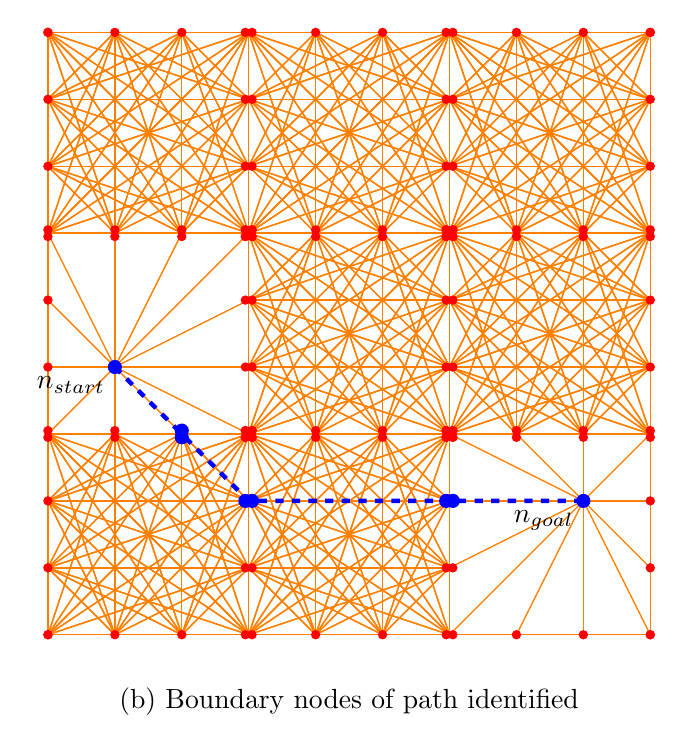
\begin{tikzpicture}[scale=0.85,line width=0.5pt]
  
      \foreach \i in {0,3,6} {
      \foreach \j in {0,3,6} {
      \foreach \x in {0,1,2,3} {
        \foreach \y in {0,3} {
          \foreach \a in {0,1,2,3} {
            \foreach \b in {0,3} {
             \pgfmathparse{int(\x + \i)};
             \let\xn\pgfmathresult;
             \pgfmathparse{int(\a + \i)};
             \let\an\pgfmathresult;
             \pgfmathparse{int(\y + \j)};
             \let\yn\pgfmathresult;
             \pgfmathparse{int(\b + \j)};
             \let\bn\pgfmathresult;
              \draw[orange] (\xn,\yn) -- (\an,\bn);
              \draw[orange] (\yn,\xn) -- (\bn,\an);
            }
          }
        }
      }
      }}
      
      \foreach \i in {0,3,6} {
      \foreach \j in {0,3,6} {
      \foreach \x in {1,2} {
        \foreach \y in {0,3} {
          \foreach \a in {1,2} {
            \foreach \b in {0,3} {
             \pgfmathparse{int(\x+\i)};
             \let\xn\pgfmathresult;
             \pgfmathparse{int(\a+\j)};
             \let\an\pgfmathresult;
             \pgfmathparse{int(\y+\j)};
             \let\yn\pgfmathresult;
             \pgfmathparse{int(\b+\i)};
             \let\bn\pgfmathresult;
              \draw[orange] (\xn,\yn) -- (\bn,\an);
              \draw[orange] (\yn,\xn) -- (\an,\bn);
            }
          }
        }
      }
      }}
      
      \filldraw[color=orange, fill=white] (0,3) rectangle (3,6);
      \filldraw[color=orange, fill=white] (6,0) rectangle (9,3);
      
      \draw[orange] (1,4) -- (0,3);
      \draw[orange] (1,4) -- (0,4);
      \draw[orange] (1,4) -- (0,5);
      \draw[orange] (1,4) -- (0,6);
      \draw[orange] (1,4) -- (3,3);
      \draw[orange] (1,4) -- (3,4);
      \draw[orange] (1,4) -- (3,5);
      \draw[orange] (1,4) -- (3,6);
      \draw[orange] (1,4) -- (1,3);
      \draw[orange] (1,4) -- (2,3);
      \draw[orange] (1,4) -- (1,6);
      \draw[orange] (1,4) -- (2,6);

      \draw[orange] (8,2) -- (6,0);
      \draw[orange] (8,2) -- (6,1);
      \draw[orange] (8,2) -- (6,2);
      \draw[orange] (8,2) -- (6,3);
      \draw[orange] (8,2) -- (9,0);
      \draw[orange] (8,2) -- (9,1);
      \draw[orange] (8,2) -- (9,2);
      \draw[orange] (8,2) -- (9,3);
      \draw[orange] (8,2) -- (7,0);
      \draw[orange] (8,2) -- (8,0);
      \draw[orange] (8,2) -- (7,3);
      \draw[orange] (8,2) -- (8,3);     
      
      \fill[red] (1,4) circle (2pt);
      \node[below left] at (1,4) {$n_{start}$};
      \fill[red] (8,2) circle (2pt);
      \node[below left] at (8,2) {$n_{goal}$};
      
      \foreach \x in {0,1,2,2.95,3.05,4,5,5.95,6.05,7,8,9} {
        \foreach \y in {0,9} {
              \fill[red] (\x,\y) circle (2pt);
              \fill[red] (\y,\x) circle (2pt);
        }
      }
      
      \foreach \x in {1,2,4,5,7,8} {
        \foreach \y in {3,6} {
          \pgfmathparse{(\y + 0.05)};
           \let\ya\pgfmathresult;
            \pgfmathparse{(\y - 0.05)};
           \let\yb\pgfmathresult;
              \fill[red] (\x,\ya) circle (2pt);
              \fill[red] (\x,\yb) circle (2pt);
              \fill[red] (\ya,\x) circle (2pt);
              \fill[red] (\yb,\x) circle (2pt);
        }
      }
      
       \foreach \x in {3,6} {
        \foreach \y in {3,6} {
          \pgfmathparse{(\x + 0.05)};
           \let\xa\pgfmathresult;
            \pgfmathparse{(\x - 0.05)};
           \let\xb\pgfmathresult;
           \pgfmathparse{(\y + 0.05)};
           \let\ya\pgfmathresult;
              \fill[red] (\xa,\ya) circle (2pt);
              \fill[red] (\xb,\ya) circle (2pt);
              \fill[red] (\ya,\xa) circle (2pt);
              \fill[red] (\ya,\xb) circle (2pt);
        }
      }
      
             \foreach \x in {3,6} {
        \foreach \y in {3,6} {
          \pgfmathparse{(\x + 0.05)};
           \let\xa\pgfmathresult;
            \pgfmathparse{(\x - 0.05)};
           \let\xb\pgfmathresult;
           \pgfmathparse{(\y - 0.05)};
           \let\ya\pgfmathresult;
              \fill[red] (\xa,\ya) circle (2pt);
              \fill[red] (\xb,\ya) circle (2pt);
              \fill[red] (\ya,\xa) circle (2pt);
              \fill[red] (\ya,\xb) circle (2pt);
        }
      }
      
      \fill[blue] (1,4) circle (3pt);
      \fill[blue] (2,3.05) circle (3pt);
      \fill[blue] (2,2.95) circle (3pt);
      \fill[blue] (2.95,2) circle (3pt);
      \fill[blue] (3.05,2) circle (3pt);
      \fill[blue] (5.95,2) circle (3pt);
      \fill[blue] (6.05,2) circle (3pt);
      \fill[blue] (8,2) circle (3pt);
      \draw[blue,ultra thick,dashed] (1,4) -- (2,3) -- (3,2) -- (6,2) -- (8,2);
      
      \node at (4.5,-1) {(b) Boundary nodes of path identified};
     
    \end{tikzpicture}
	    };
	    
\node (c) at (0,0) {
    	    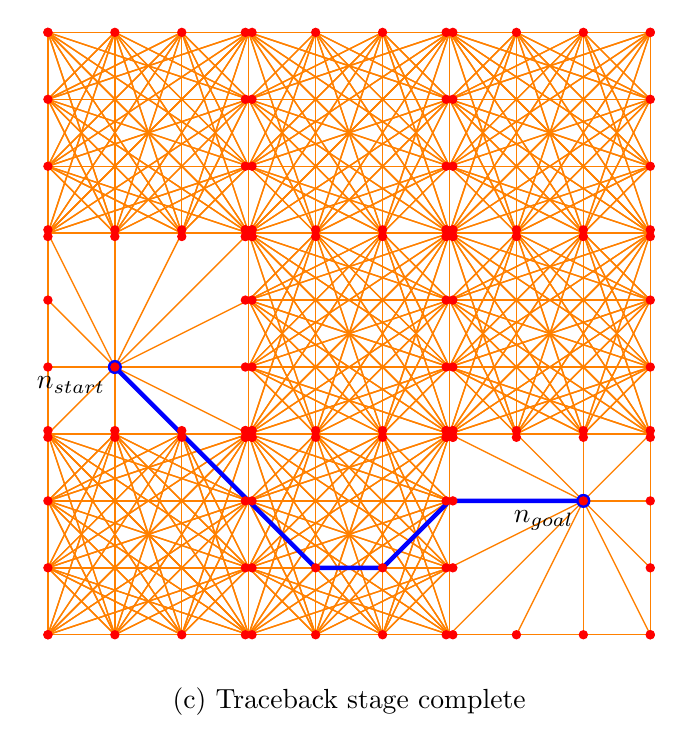
\begin{tikzpicture}[scale=0.85,line width=0.5pt]
  
      \foreach \i in {0,3,6} {
      \foreach \j in {0,3,6} {
      \foreach \x in {0,1,2,3} {
        \foreach \y in {0,3} {
          \foreach \a in {0,1,2,3} {
            \foreach \b in {0,3} {
             \pgfmathparse{int(\x + \i)};
             \let\xn\pgfmathresult;
             \pgfmathparse{int(\a + \i)};
             \let\an\pgfmathresult;
             \pgfmathparse{int(\y + \j)};
             \let\yn\pgfmathresult;
             \pgfmathparse{int(\b + \j)};
             \let\bn\pgfmathresult;
              \draw[orange] (\xn,\yn) -- (\an,\bn);
              \draw[orange] (\yn,\xn) -- (\bn,\an);
            }
          }
        }
      }
      }}
      
      \foreach \i in {0,3,6} {
      \foreach \j in {0,3,6} {
      \foreach \x in {1,2} {
        \foreach \y in {0,3} {
          \foreach \a in {1,2} {
            \foreach \b in {0,3} {
             \pgfmathparse{int(\x+\i)};
             \let\xn\pgfmathresult;
             \pgfmathparse{int(\a+\j)};
             \let\an\pgfmathresult;
             \pgfmathparse{int(\y+\j)};
             \let\yn\pgfmathresult;
             \pgfmathparse{int(\b+\i)};
             \let\bn\pgfmathresult;
              \draw[orange] (\xn,\yn) -- (\bn,\an);
              \draw[orange] (\yn,\xn) -- (\an,\bn);
            }
          }
        }
      }
      }}
      
      \filldraw[color=orange, fill=white] (0,3) rectangle (3,6);
      \filldraw[color=orange, fill=white] (6,0) rectangle (9,3);
      
      \draw[orange] (1,4) -- (0,3);
      \draw[orange] (1,4) -- (0,4);
      \draw[orange] (1,4) -- (0,5);
      \draw[orange] (1,4) -- (0,6);
      \draw[orange] (1,4) -- (3,3);
      \draw[orange] (1,4) -- (3,4);
      \draw[orange] (1,4) -- (3,5);
      \draw[orange] (1,4) -- (3,6);
      \draw[orange] (1,4) -- (1,3);
      \draw[orange] (1,4) -- (2,3);
      \draw[orange] (1,4) -- (1,6);
      \draw[orange] (1,4) -- (2,6);

      \draw[orange] (8,2) -- (6,0);
      \draw[orange] (8,2) -- (6,1);
      \draw[orange] (8,2) -- (6,2);
      \draw[orange] (8,2) -- (6,3);
      \draw[orange] (8,2) -- (9,0);
      \draw[orange] (8,2) -- (9,1);
      \draw[orange] (8,2) -- (9,2);
      \draw[orange] (8,2) -- (9,3);
      \draw[orange] (8,2) -- (7,0);
      \draw[orange] (8,2) -- (8,0);
      \draw[orange] (8,2) -- (7,3);
      \draw[orange] (8,2) -- (8,3);   
      
      \draw[blue,ultra thick] (1,4) -- (2,3) -- (3,2) -- (4,1) -- (5,1) -- (6,2) -- (8,2);
      \fill[blue] (1,4) circle (3pt);
      \fill[blue] (8,2) circle (3pt);
      \fill[red] (4,1) circle (2pt);
      \fill[red] (5,1) circle (2pt);
      
      \fill[red] (1,4) circle (2pt);
      \node[below left] at (1,4) {$n_{start}$};
      \fill[red] (8,2) circle (2pt);
      \node[below left] at (8,2) {$n_{goal}$};
      
      \foreach \x in {0,1,2,2.95,3.05,4,5,5.95,6.05,7,8,9} {
        \foreach \y in {0,9} {
              \fill[red] (\x,\y) circle (2pt);
              \fill[red] (\y,\x) circle (2pt);
        }
      }
      
      \foreach \x in {1,2,4,5,7,8} {
        \foreach \y in {3,6} {
          \pgfmathparse{(\y + 0.05)};
           \let\ya\pgfmathresult;
            \pgfmathparse{(\y - 0.05)};
           \let\yb\pgfmathresult;
              \fill[red] (\x,\ya) circle (2pt);
              \fill[red] (\x,\yb) circle (2pt);
              \fill[red] (\ya,\x) circle (2pt);
              \fill[red] (\yb,\x) circle (2pt);
        }
      }
      
       \foreach \x in {3,6} {
        \foreach \y in {3,6} {
          \pgfmathparse{(\x + 0.05)};
           \let\xa\pgfmathresult;
            \pgfmathparse{(\x - 0.05)};
           \let\xb\pgfmathresult;
           \pgfmathparse{(\y + 0.05)};
           \let\ya\pgfmathresult;
              \fill[red] (\xa,\ya) circle (2pt);
              \fill[red] (\xb,\ya) circle (2pt);
              \fill[red] (\ya,\xa) circle (2pt);
              \fill[red] (\ya,\xb) circle (2pt);
        }
      }
      
             \foreach \x in {3,6} {
        \foreach \y in {3,6} {
          \pgfmathparse{(\x + 0.05)};
           \let\xa\pgfmathresult;
            \pgfmathparse{(\x - 0.05)};
           \let\xb\pgfmathresult;
           \pgfmathparse{(\y - 0.05)};
           \let\ya\pgfmathresult;
              \fill[red] (\xa,\ya) circle (2pt);
              \fill[red] (\xb,\ya) circle (2pt);
              \fill[red] (\ya,\xa) circle (2pt);
              \fill[red] (\ya,\xb) circle (2pt);
        }
      }
      
      \node at (4.5,-1) {(c) Traceback stage complete};
      
     
    \end{tikzpicture}
	    };
	    
\node (d) at (10,0) {
    	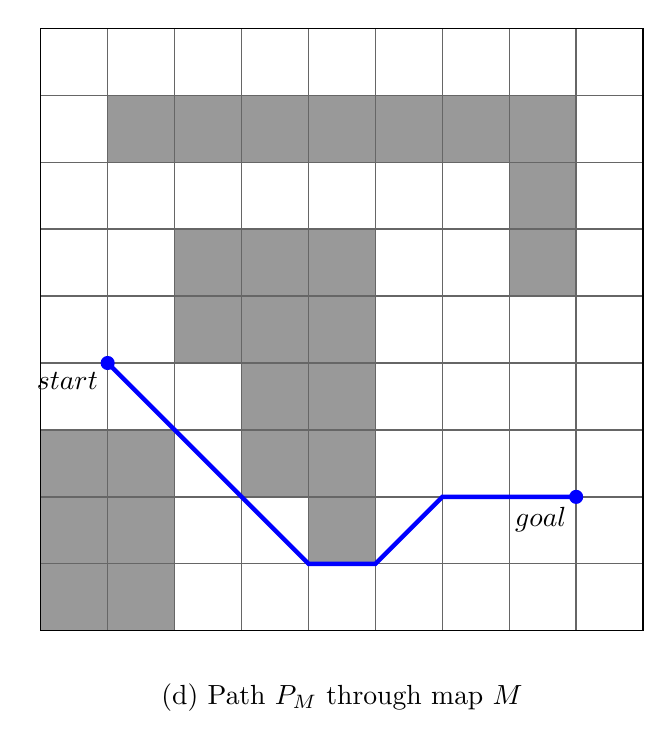
\begin{tikzpicture}[scale=0.85,line width=0.5pt]
	      	\filldraw[color=black!60,fill=black!40] (0,0) rectangle (2,3); 
		\filldraw[color=black!60,fill=black!40] (1,7) rectangle (8,8); 
		\filldraw[color=black!60,fill=black!40] (7,7) rectangle (8,5); 
		\filldraw[color=black!60,fill=black!40] (2,4) rectangle (5,6);
		\filldraw[color=black!60,fill=black!40] (3,2) rectangle (5,4); 
		\filldraw[color=black!60,fill=black!40] (4,1) rectangle (5,2);  
     	 	\draw[color=black!60] (0,0) grid (9,9);
      		\draw[black] (0,0) -- (0,9);
      		\draw[black] (0,0) -- (9,0);
      		\draw[black] (9,9) -- (0,9);
      		\draw[black] (9,9) -- (9,0);
		\node[below left] at (1,4) {$start$};
		\node[below left] at (8,2) {$goal$};
		\fill[blue] (1,4) circle (3pt);
      		\fill[blue] (8,2) circle (3pt);
      		\draw[blue,ultra thick] (1,4) -- (2,3) -- (3,2) -- (4,1) -- (5,1) -- (6,2) -- (8,2);
		
		\node at (4.5,-1) {(d) Path $P_{M}$ through map $M$};
	    \end{tikzpicture}
	    };	

    \end{tikzpicture}
    \caption[Solution of {\em Block A*}]{Solution of {\em Block A*}}
  %\label{fig:fig}
\end{figure}


\clearpage
\section {Requirements analysis}

As specified in the {\bfseries Project Proposal} (see Appendix B), this project is logically composed of four parts. This section outlines the functional and non-functional requirements for each part, and their relative priorities using the MoSCoW system. \\
\centerline {M - Must; S - Should; C - Could; W - Won't}

\subsection{Testing simulator}

\begin{center}
\begin{tabular}{@{}l p{10cm} cccc} \toprule
\multicolumn{2}{r}{~} &\multicolumn{4}{c}{Priority} \\ 
\cmidrule(l){3-6}
ID & Functional requirements & M & S & C & W  \\ \midrule
    1 & The system shall load one of a collection of maps from the generator & \cellcolor{green!60} & ~ & ~ & ~\\
    2 & The system shall allow maps to be saved so that multiple tests can be run on the same map suite & ~ & \cellcolor{yellow!80} & ~ & ~ \\    
   3 & The system shall create a grid-graph from a given map & \cellcolor{green!60} & ~ & ~ & ~\\
   4 & The system shall create a visibility graph from a given map & ~ & ~ & \cellcolor{orange!60} & ~\\
   5 & The system shall run one of a collection of any-angle path-finding algorithms on a graph and collect data such as the path-length and the length of computation & \cellcolor{green!60} & ~ & ~ & ~\\
    6 & The system shall display a visual representation of the current map and the paths found by any algorithms that have been run on it & \cellcolor{green!60} & ~ & ~ & ~\\
    7 & The system shall display the numeric statistics for each path for the current map & \cellcolor{green!60} & ~ & ~ & ~\\
    \midrule
    ~ & Non-functional requirements & \multicolumn{4}{r}{}  \\ \midrule
    1 & The system shall be designed in a modular way to allow easy extension for new algorithms & ~ & \cellcolor{yellow!80} & ~ & ~ \\  \bottomrule
\end{tabular}
\end{center}

\subsection{Map generation}

\begin{center}
        \begin{tabular}{@{}l p{10cm} cccc} \toprule
\multicolumn{2}{r}{~} &\multicolumn{4}{c}{Priority} \\ 
\cmidrule(l){3-6}
ID & Functional requirements & M & C & S & W  \\ \midrule
    1 & The system shall generate pseudo-random maps of a given resolution, coverage percentage and clustering & \cellcolor{green!60} & ~ & ~ & ~\\
    2 & The system shall allow maps to be saved so that multiple tests can be run on the same map suite & \cellcolor{green!60} & ~ & ~ & ~\\
    3 & The system shall allow maps to be created with an interactive map editor & ~ & ~ & \cellcolor{orange!60} & ~\\
    \midrule
    ~ & Non-functional requirements & \multicolumn{4}{r}{}  \\ \midrule
    1 & The system shall generate maps of the highest resolution in under 2 seconds & ~ & \cellcolor{yellow!80} & ~ & ~ \\  \bottomrule
\end{tabular}
\end{center}
	
\subsection{Algorithm implementation}

\begin{center}
    \begin{tabular}{@{}l p{10cm} cccc} \toprule
\multicolumn{2}{r}{~} &\multicolumn{4}{c}{Priority} \\ 
\cmidrule(l){3-6}
ID & Functional requirements & M & C & S & W  \\ \midrule
1 & The system shall correctly implement each of the chosen algorithms. If a path exists, the path and numerical statistics will be returned. If no path exists, this will be returned & \cellcolor{green!60} & ~ & ~ & ~\\
    2 & The system shall allow arbitrary start and end coordinates for any map & ~ & \cellcolor{yellow!80} & ~ & ~ \\ 
    \midrule
    ~ & Non-functional requirements & \multicolumn{4}{r}{}  \\ \midrule
    1 & he system shall be designed in a modular way to allow easy extension for new algorithms & ~ & \cellcolor{yellow!80} & ~ & ~ \\  \bottomrule
\end{tabular}
\end{center}

\subsection{Data gathering}

\begin{center}
    \begin{tabular}{@{}l p{10cm} cccc} \toprule
\multicolumn{2}{r}{~} &\multicolumn{4}{c}{Priority} \\ 
\cmidrule(l){3-6}
ID & Functional requirements & M & C & S & W  \\ \midrule
    1 & The system shall write statistics for an arbitrary set of specified algorithms on an arbitrary set of specified maps and write the results to a CSV file & \cellcolor{green!60} & ~ & ~ & ~\\
    \midrule
    ~ & Non-functional requirements & \multicolumn{4}{r}{}  \\ \midrule
    1 & The system shall be designed with a clear API that enables quick and easy data gathering & \cellcolor{green!60} & ~ & ~ & ~\\ \bottomrule
\end{tabular}
\end{center}

\section {Design model}

\noindent
The plan for the implementation phase was refined from that presented in the {\bfseries Project Proposal} (see Appendix B). An incremental model of implementation was adopted, with new modules being developed and tested separately before being integrated into the work program. The milestones of the project were:
\begin{description}
\item[Milestone 1]\hfil \\
Maps of arbitrary size, coverage and clustering can be created and printed to system output.
\item[Milestone 2]\hfil \\
Arbitrary maps can be converted to graphs, and {\em Dijkstra} and {\em A*} can be run on these maps. A visual representation of the path can be printed to system output.
\item[Milestone 3]\hfil \\
Basic UI is built, including all functionality from {\bfseries Milestone 2}. Basic path statistics are displayed.
\item[Milestone 4]\hfil \\
Map saving, map loading and map creation functionality are present. This will facilitate debugging edge cases for more complex algorithms.
\item[Milestone 5]\hfil \\
{\em A* with post-smoothing}, {\em Theta*} and {\em Lazy Theta*} are implemented.
\item[Milestone 6]\hfil \\
{\em Block A*} is implemented.
\item[Milestone 7]\hfil \\
Data extraction scripts are implemented.
\end{description}

\section {Languages and tools}

This section justifies the languages, libraries and tools that were chosen for this project.

\begin{description}
  \item[Programming language] \hfill \\
  {\em Java} --- provides abstraction and class hierarchy to enable development of modular, extensible code. Various libraries were used, including:\\
  \hphantom{} \hspace{6 mm}{\em Swing} --- for graphical user interface design;\\ 
  \hphantom{} \hspace{6 mm}{\em CSVWriter} --- for data export;\\
  \hphantom{} \hspace{6 mm}{\em JUnit} --- for unit testing.
  \item[Integrated development environment] \hfill \\
  {\em Eclipse} --- allows rapid development through integrated testing, refactoring and version control tools.
  \item[Statistical analysis and visualisation] \hfill \\
  {\em R} --- open-source statistical package; chosen due to its flexibility and extensibility.
  \item[Document preparation] \hfill \\
  {\LaTeX} --- allows precise, integrated control over all aspects of document layout and style. Various packages were used, including:\\
  \hphantom{} \hspace{6 mm}{\em Tikz} --- enables programmable diagram creation;\\
  \hphantom{} \hspace{6 mm}{\em algorithm2e} --- enables integration with the parent document;\\
  \hphantom{} \hspace{6 mm}{\em listings} --- displays colour formatted code for a range of programming languages;\\
  \hphantom{} \hspace{6 mm}{\em todonotes} --- enables clear organisation of tasks that haven't been completed.
  \item[Backup] \hfill \\
  {\em DropBox} and {\em Google Drive} --- maintain multiple shadow copies of my work in the cloud.
  \item[Version Control]\hfill \\
  {\em GitHub} --- facilitated exploring different implementation strategies by forking my core code repository.
  
\end{description}

%\cleardoublepage
\chapter{Implementation}

This chapter provides an overview of the implementation of the project and explores some of the more interesting parts in further detail.\\

\noindent
Figure 3.1 provides an simplified view of the flow of the user interface and engine of the program, and is included to serve as a useful framework with which to describe the implementation of the program.\\

\noindent
The basic control flow upon which Figure 3.1 is based is explained below:
\begin{itemize}
\item {\bfseries Map \& algorithm selection} --- the user selects a map using one of the three methods below, selects a $start$ and $goal$ location and selects an pathfinding algorithm.
  \begin{itemize}
  \item {\bfseries MapGenerator} --- allows the program to automatically generate a map according to user-selected parameters;
  \item {\bfseries MapCreator} --- creates the map using a `paint brush' style editor;
  \item {\bfseries MapLoader} --- loads a map that has been previously saved;
  \end{itemize}
\item {\bfseries GraphGenerator} --- the system creates a graph representation of the map;
\item {\bfseries Pathfinding algorithm} --- the system runs the selected pathfinding algorithm on the graph;
\item {\bfseries Visualizer} --- the system displays the path, and statistics about the path, in the visualiser;
\item {\bfseries Data export} --- the statistics about the path may be exported in CSV format.
\end{itemize}

\begin{figure}
  \centering
  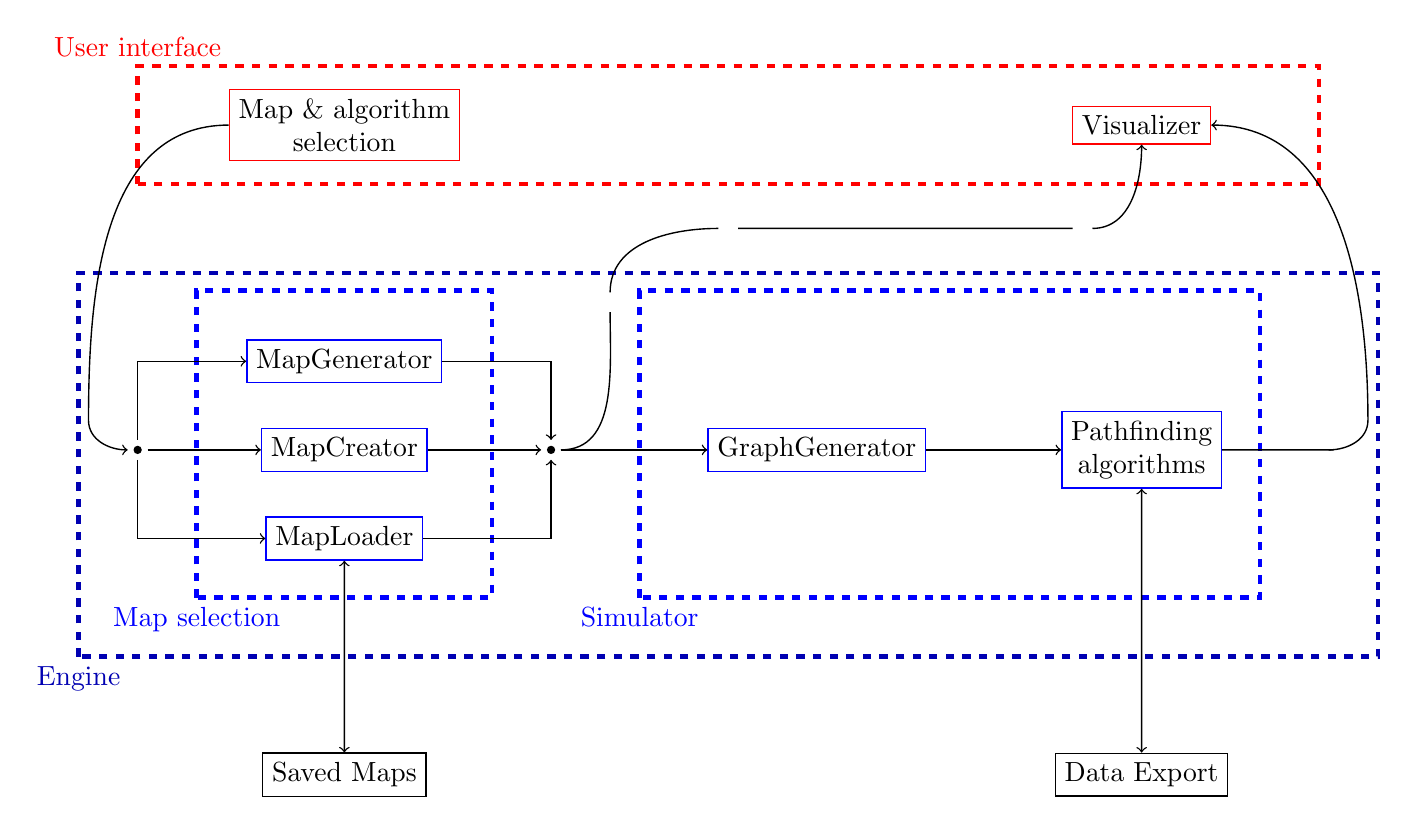
\begin{tikzpicture}[scale=0.75,line width=0.5pt]
  \filldraw[color=red,fill=white,dashed, ultra thick] (0,5) rectangle (20,7); 
  \node[above, red] at (0,7) {User interface};
  \filldraw[color=blue!70!black,fill=white,dashed, ultra thick] (-1,-3) rectangle (21,3.5); 
  \node[below, blue!70!black] at (-1,-3) {Engine};
  \filldraw[color=blue,fill=white,dashed, ultra thick] (1,-2) rectangle (6,3.2); 
  \node[below, blue] at (1,-2) {Map selection};
  \filldraw[color=blue,fill=white,dashed, ultra thick] (8.5,-2) rectangle (19,3.2); 
  \node[below, blue] at (8.5,-2) {Simulator};
  
\node[draw=red,shape=rectangle,align=center] at (3.5,6) (MapAlgSelection) {Map \& algorithm \\selection};
\node at (-1,1) (LeftCurveNode) {};
\fill (0,0.5) circle (2pt);
\node at (0,0.5) (LeftCurveEnd) {};
\node[draw=blue,shape=rectangle,align=center] at (3.5,2) (MapGenerator) {MapGenerator};
\node[draw=blue,shape=rectangle,align=center] at (3.5,0.5) (MapCreator) {MapCreator};
\node[draw=blue,shape=rectangle,align=center] at (3.5,-1) (MapLoader) {MapLoader};
\draw[->] (LeftCurveEnd) |- (MapGenerator);
\draw[->] (LeftCurveEnd) to (MapCreator);
\draw[->] (LeftCurveEnd) |- (MapLoader);
\node at (7,0.5) (InternalNode) {};
\fill (7,0.5) circle (2pt);
\draw[->] (MapGenerator) -| (InternalNode);
\draw[->] (MapCreator) to (InternalNode);
\draw[->] (MapLoader) -| (InternalNode);
\node[draw=blue,shape=rectangle,align=center] at (11.5,0.5) (GraphGenerator) {GraphGenerator};
\draw[->] (InternalNode) to (GraphGenerator);
\node[draw=blue,shape=rectangle,align=center] at (17,0.5) (PathfindingAlgorithms) {Pathfinding \\algorithms};
\draw[->] (GraphGenerator) to (PathfindingAlgorithms);
\node at (20,0.5) (1) {};
\node at (21,1) (RightCurveNode) {};
\draw (PathfindingAlgorithms) to (20.25,0.5);
\node[draw=red,shape=rectangle,align=center] at (17,6) (Visualizer) {Visualizer};
\node at (8,3) (2) {};
\node at (10,4.25) (3) {};
\node at (16,4.25) (4) {};
\draw[->] (InternalNode.east) to[out=0,in=-90] (2) to[out=90,in=180] (3) to[out=0,in=180] (4) to[out=0, in=-90] (Visualizer.south);
\node[draw=black,shape=rectangle,align=center] at (3.5,-5) (SavedMaps) {Saved Maps};
\node[draw=black,shape=rectangle,align=center] at (17,-5) (DataExport) {Data Export};

\draw[->] (MapAlgSelection.west) to[out=180,in=90] (LeftCurveNode.east) to[out=-90,in=180] (LeftCurveEnd.west);
\draw[->] (1.east) to[out=0,in=-90] (RightCurveNode.west) to[out=90,in=0] (Visualizer.east);
\draw[<->] (MapLoader) to (SavedMaps);
\draw[<->] (PathfindingAlgorithms) to (DataExport);


  \end{tikzpicture}
  \caption{Flow of the user interface and engine} 
\end{figure}

\section{Map selection}

This section introduces how maps are implemented, and the three methods of selecting a map --- map generation, map creation, and loading a previously saved map.\\

\subsection{Maps}
A map is implemented with a {\tt Map} object, which is a square array of {\tt Cell} objects. Each {\tt Cell} object has a boolean instance variable that records whether or not that cell is blocked.

\subsection{Map generation}
The system provides a module to automatically generate maps according to a given set of parameters, which define the size $N \times N$ of the map, the percentage $C$ of the cells of the map that are blocked, and a clustering score $D$ which defines how likely the blocked cells are to be found in clusters as opposed to spaced evenly throughout the map. This facility is required so that large volumes of maps can be created to allow rigorous statistical analysis of the algorithms over maps with certain known properties. The bespoke algorithm devised for this project to pseudo-randomly create such maps is now explained.\\

\noindent{\bfseries Overview}\\
\noindent
Starting with a blank map (i.e. a map where every cell is free), each iteration of the algorithm chooses one unblocked cell of the map to be blocked, until $C\%$ of the cells have been blocked --- i.e. until $C/N^{2}$ iterations have completed. To record which cells were blocked on previous iterations and to decide which cell to block on the next iteration, the algorithm maintains a matrix $m$ of size $N \times N$, where at any point in the algorithm the value of element $m_{x,y}$ represents the `potential' of cell $(x,y)$ --- where the potential of element $m_{x,y}$ represents the relative probability that $(x,y)$ will be chosen to be blocked on the next iteration. To be more precise: 
\begin{equation}
P((x,y) \mbox{chosen to be blocked on the next iteration}) = m_{x,y}/\sum\limits_{i,j} m_{i,j}
\end{equation}
\noindent
Initially, the potential of every cell is 1, to represent that there is an equal chance of $1/N^{2}$ of any cell being chosen to be blocked in the first iteration.\\

\begin{figure}
\centering
  \begin{subfigure}{.49\textwidth}
  \centering
  {\includegraphics[width=0.49\textwidth]{clustering0_.png}}
  \caption{$D=0$}
  \end{subfigure}
  \begin{subfigure}{.49\textwidth}
  \centering
  {\includegraphics[width=0.49\textwidth]{clustering50_.png}}
  \caption{$D=50$}
  \end{subfigure}
  \caption[Close up of generated maps]{Close up of generated maps of coverage $C=30\%$ and different clustering scores $D$} 
\end{figure}

\noindent
If cell $(x,y)$ is chosen to be blocked, $m_{x,y}$ is set to $0$ to ensure that it cannot be chosen again, and the potentials of the eight cells that surround $(x,y)$ are increased by a value which depends on the clustering score $D$, to ensure that if $D > 0$ then subsequent iterations are more likely to block cells that are spatially close to cells that were blocked on previous iterations, and hence create clusters of blocked cells. The amount by which the potentials of the cells surrounding $(x,y)$ are increased when $(x,y)$ is blocked models a crude approximation of a potential field, or gravity well, around $(x,y)$.\\

\begin{figure}
\centering
  \begin{subfigure}[b]{0.49\textwidth}
  \centering
  \begin{tikzpicture}
    \node[above right] at (0,0) {
    \begin{tikzpicture}
    \begin{scope}
    \clip(-2.5,-2.5) rectangle (2.5,2.5);
    \foreach \x in {100,...,350} {
    	  \pgfmathparse{\x / 100};
          \let\xa\pgfmathresult;
          \pgfmathparse{\xa};
          \let\xb\pgfmathresult;
          \pgfmathparse{1/ (\xb * \xb)};
          \let\xc\pgfmathresult;
          \pgfmathparse{100 * \xc}; 
          \let\xd\pgfmathresult;
          \draw[color=red!\xd] (0,0) circle (\xa);
      }
        \foreach \y in {1,...,100} {
    	  \pgfmathparse{\y / 100};
          \let\ya\pgfmathresult;
          \pgfmathparse{\ya *100};
          \let\yb\pgfmathresult;
          \draw[color=red!\yb] (0,0) circle (\ya);
          }
      \end{scope}
      
      \draw[color=black!60] (-2.5,-2.5) -- (2.5,-2.5);
      \draw[color=black!60] (-2.5,-1.5) -- (2.5,-1.5);
      \draw[color=black!60] (-2.5,-0.5) -- (2.5,-0.5);
      \draw[color=black!60] (-2.5,0.5) -- (2.5,0.5);
      \draw[color=black!60] (-2.5,1.5) -- (2.5,1.5);
      \draw[color=black!60] (-2.5,2.5) -- (2.5,2.5);
      
      \draw[color=black!60] (-2.5,-2.5) -- (-2.5,2.5);
      \draw[color=black!60] (-1.5,-2.5) -- (-1.5,2.5);
      \draw[color=black!60] (-0.5,-2.5) -- (-0.5,2.5);
      \draw[color=black!60] (0.5,-2.5) -- (0.5,2.5);
      \draw[color=black!60] (1.5,-2.5) -- (1.5,2.5);
      \draw[color=black!60] (2.5,-2.5) -- (2.5,2.5);
      
      \end{tikzpicture}
      };
      
      \node[below] at (2.5,0) {overhead view};
      
      \node[above right] at (0,-3.5) {
    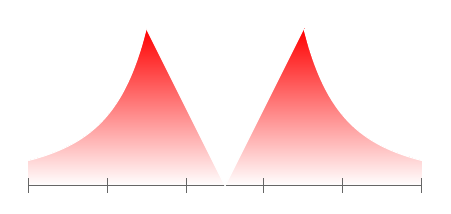
\begin{tikzpicture}
      \foreach \x in {1,...,160} {
    	  \pgfmathparse{\x / 1000};
          \let\xa\pgfmathresult;
          \pgfmathparse{\xa * 2};
          \let\xb\pgfmathresult;
          \pgfmathparse{1 / sqrt(\xa)};
          \let\xc\pgfmathresult;
          \pgfmathparse{\xb * 50};
          \let\xd\pgfmathresult;
          \pgfmathparse{-1*\xa};
          \let\xe\pgfmathresult;
          \pgfmathparse{-1*\xc};
          \let\xf\pgfmathresult;
          \draw[color=red!\xd] (\xa,\xb) -- (2.5,\xb);
          \draw[color=red!\xd] (\xe,\xb) -- (-2.5,\xb);
      }
      \foreach \x in {160,...,1000} {
    	  \pgfmathparse{\x / 1000};
          \let\xa\pgfmathresult;
          \pgfmathparse{\xa * 2};
          \let\xb\pgfmathresult;
          \pgfmathparse{1 / sqrt(\xa)};
          \let\xc\pgfmathresult;
          \pgfmathparse{\xb * 50};
          \let\xd\pgfmathresult;
          \pgfmathparse{-1*\xa};
          \let\xe\pgfmathresult;
          \pgfmathparse{-1*\xc};
          \let\xf\pgfmathresult;
          \draw[color=red!\xd] (\xa,\xb) -- (\xc,\xb);
          \draw[color=red!\xd] (\xe,\xb) -- (\xf,\xb);
      }

  \draw[|-|, color=black!60] (-2.5,0) -- (2.5,0);
  \draw[|-|, color=black!60] (-1.5,0) -- (1.5,0);
  \draw[|-|, color=black!60] (-0.5,0) -- (0.5,0);
  \draw[domain=1:2.5,smooth,variable=\x,white] plot ({\x},{2*(1 / (\x * \x))});
  \draw[domain=-2.5:-1,smooth,variable=\x,white] plot ({\x},{2*(1 / (\x * \x))});
  \draw[domain=0:1,smooth,variable=\x,white] plot ({\x},{2*(\x)});
  \draw[domain=-1:0,smooth,variable=\x,white] plot ({\x},{2*(-1* \x)});
      \end{tikzpicture}
      };
      
      \node[below] at (2.5,-3.5) {cross-section};
      
\end{tikzpicture}

  \caption{Gravity well}
  \end{subfigure}
  \begin{subfigure}[b]{0.49\textwidth}
  \centering
  \begin{tikzpicture}
\node[above right] at (0,0) {
    \begin{tikzpicture}

      \filldraw[red!50] (-1.5,-1.5) rectangle (-0.5,-0.5);
      \filldraw[red!50] (0.5,-1.5) rectangle (1.5,-0.5);
      \filldraw[red!50] (-1.5,0.5) rectangle (-0.5,1.5);
      \filldraw[red!50] (0.5,0.5) rectangle (1.5,1.5);

      \filldraw[red] (-0.5,-1.5) rectangle (0.5,-0.5);
      \filldraw[red] (-1.5,-0.5) rectangle (-0.5,0.5);
      \filldraw[red] (0.5,-0.5) rectangle (1.5,0.5);
      \filldraw[red] (-0.5,0.5) rectangle (0.5,1.5);
      
      \draw[color=black!60] (-2.5,-2.5) -- (2.5,-2.5);
      \draw[color=black!60] (-2.5,-1.5) -- (2.5,-1.5);
      \draw[color=black!60] (-2.5,-0.5) -- (2.5,-0.5);
      \draw[color=black!60] (-2.5,0.5) -- (2.5,0.5);
      \draw[color=black!60] (-2.5,1.5) -- (2.5,1.5);
      \draw[color=black!60] (-2.5,2.5) -- (2.5,2.5);
      
      \draw[color=black!60] (-2.5,-2.5) -- (-2.5,2.5);
      \draw[color=black!60] (-1.5,-2.5) -- (-1.5,2.5);
      \draw[color=black!60] (-0.5,-2.5) -- (-0.5,2.5);
      \draw[color=black!60] (0.5,-2.5) -- (0.5,2.5);
      \draw[color=black!60] (1.5,-2.5) -- (1.5,2.5);
      \draw[color=black!60] (2.5,-2.5) -- (2.5,2.5);
      \end{tikzpicture}
      };
      
      \node[below] at (2.5,0) {overhead view};
      
      \node[above right] at (0,-3.5) {
    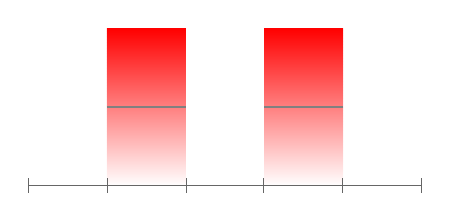
\begin{tikzpicture}
\foreach \x in {0,...,1000} {
    	  \pgfmathparse{\x / 500};
          \let\xa\pgfmathresult;
          \pgfmathparse{\xa * 50};
          \let\xb\pgfmathresult;
          
          \draw[color=red!\xb] (1.5,\xa) -- (0.5,\xa);
          \draw[color=red!\xb] (-1.5,\xa) -- (-0.5,\xa);
      }
  \draw[|-|, color=black!60] (-2.5,0) -- (2.5,0);
  \draw[|-|, color=black!60] (-1.5,0) -- (1.5,0);
  \draw[|-|, color=black!60] (-0.5,0) -- (0.5,0);
  \draw[gray](-1.5,1) -- (-0.5,1);
  \draw[gray] (1.5,1) -- (0.5,1);
\end{tikzpicture}
};
\node[below] at (2.5,-3.5) {cross-section};

      
\end{tikzpicture}

  \caption{Approximation}
  \end{subfigure}
\caption{The potential field of a gravity well and an approximation to a gravity well}
\end{figure}

\noindent{\bfseries Implementation}\\
\noindent
A single iteration of the algorithm, which is given in the {\bfseries repeat \ldots until} block in the pseudo-code in Algorithm 7, can now be summarised: a random number $r$ between $0$ and $\sum\limits_{i,j} m_{i,j}$ is selected, and $m$ is traversed row-by-row until the cumulative sum of the potentials of the elements traversed is at least $r$, at which point the traversal stops and the cell that has been reached is set as blocked.\\

\noindent
Now that $(x,y)$ has been chosen as the cell to be blocked, the potentials of $(x,y)$ and the surrounding eight cells are modified according to the gravity well model (i.e. $m_{x,y}$ is set to $0$, the horizontal neighbours $m_{x-1,y}$, $m_{x+1,y}$ and the vertical neighbours $m_{x,y-1}$ and $m_{x,y+1}$ are increased by $2D$ and the diagonal neighbours $m_{x-1,y-1}$, $m_{x+1,y-1}$, $m_{x+1,y+1}$ and $m_{x-1,y+1}$ are increased by $D$), and the next iteration commences.\\

\noindent
After $C/N^{2}$ iteration, $C\%$ of the cells of the map are blocked, and the algorithm terminates.

\begin{algorithm}
  \SetAlgoLined\DontPrintSemicolon
  \SetKwFunction{genMap}{GenerateMap} \SetKwFunction{setBlocked}{SetAsBlocked}
  \SetKwProg{myDef}{def}{}{}
  \myDef{\genMap{$m, C, D$}}{
    \nl \Repeat{$(C / N^{2}) times$} {
      \nl $r \gets random(0,\sum\limits_{i,j} m_{i,j})$\;
      \nl $i,j \gets 0$\;
      \nl \While{$r\geq 0$} {
        \nl $r \gets r - m_{i,j}$\;
        \nl \uIf{$i < R-1$} {
          \nl $i \gets i+1$\;
        } \nl \Else {
          \nl $i \gets 0$\;
          \nl $j \gets j+1$\;
        }
     }
     \nl \setBlocked{$i,j$};     
  }
  }
  \myDef{\setBlocked{$m_{i,j}$}} {
    \nl $m_{i,j} \gets 0$\;
    \nl \ForEach {$m_{k,l}$ in $horizontalOrVerticalNeighbour(m_{i,j})$} {
      \nl \uIf{$m_{k,l} \neq 0$} {
        \nl $m_{k,l} \gets m_{k,l} + D$\;
      }
  }
  \nl \ForEach {$ m_{k,l}$ in  $diagonalNeighbour(m_{i,j})$} {
      \nl \uIf{$m_{k,l} \neq 0$} {
        $m_{k,l} \gets a_{k,l} + 2\times D$\;
      }
  }
}
\caption{{\sc GenerateMap}}
 \end{algorithm} 
 
 \begin{figure}
\begin{subfigure}{.3\textwidth}
    \centering
    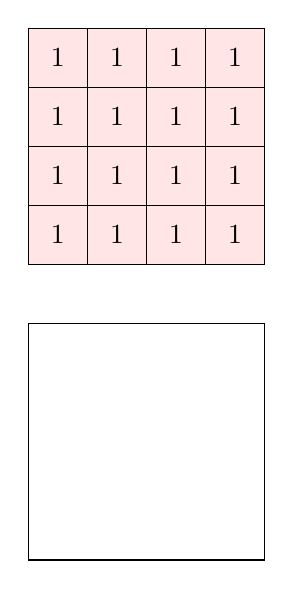
\begin{tikzpicture}[scale=0.75,line width=0.5pt]

     \filldraw[color=red!10] (0,0) rectangle (4,4); 
     \draw (0,0) grid (4,4);
    
     \foreach \x in {0,1,2,3} {
        \foreach \y in {0,1,2,3} {
          \pgfmathparse{(\x + 0.5)};
          \let\xa\pgfmathresult;
          \pgfmathparse{\y + 0.5};
          \let\ya\pgfmathresult;
          \node at (\xa,\ya) {1};
        }
      }
      
      \draw[black] (0,-5) -- (4,-5);
      \draw[black] (0,-5) -- (0,-1);
      \draw[black] (4,-1) -- (4,-5);
      \draw[black] (4,-1) -- (0,-1);
           
    \end{tikzpicture}
    \caption{Initialisation}
    %\label{fig:sfig1}
  \end{subfigure}
  \begin{subfigure}{.3\textwidth}
    \centering
    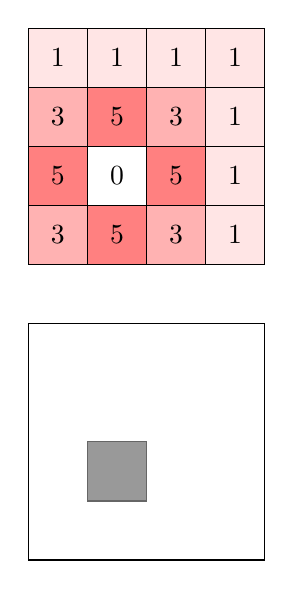
\begin{tikzpicture}[scale=0.75,line width=0.5pt]
    
    \filldraw[color=red!30] (0,0) rectangle (1,1);        
    \node at (0.5,0.5) {3};
    \filldraw[color=red!50] (1,0) rectangle (2,1); 
    \node at (1.5,0.5) {5};
    \filldraw[color=red!30] (2,0) rectangle (3,1); 
    \node at (2.5,0.5) {3};
    \filldraw[color=red!10] (3,0) rectangle (4,1); 
    \node at (3.5,0.5) {1};
    \filldraw[color=red!50] (0,1) rectangle (1,2); 
    \node at (0.5,1.5) {5};
    \filldraw[color=white] (1,1) rectangle (2,2); 
    \node at (1.5,1.5) {0};
    \filldraw[color=red!50] (2,1) rectangle (3,2); 
    \node at (2.5,1.5) {5};
    \filldraw[color=red!10] (3,1) rectangle (4,2); 
    \node at (3.5,1.5) {1};
    \filldraw[color=red!30] (0,2) rectangle (1,3); 
    \node at (0.5,2.5) {3};
    \filldraw[color=red!50] (1,2) rectangle (2,3); 
    \node at (1.5,2.5) {5};
    \filldraw[color=red!30] (2,2) rectangle (3,3); 
    \node at (2.5,2.5) {3};
    \filldraw[color=red!10] (3,2) rectangle (4,3); 
    \node at (3.5,2.5) {1};
    \filldraw[color=red!10] (0,3) rectangle (1,4); 
    \node at (0.5,3.5) {1};
    \filldraw[color=red!10] (1,3) rectangle (2,4); 
    \node at (1.5,3.5) {1};
    \filldraw[color=red!10] (2,3) rectangle (3,4); 
    \node at (2.5,3.5) {1};
    \filldraw[color=red!10] (3,3) rectangle (4,4); 
    \node at (3.5,3.5) {1};

    \draw (0,0) grid (4,4);
    
     \filldraw[color=black!60,fill=black!40] (1,-4) rectangle (2,-3); 
      
      \draw[black] (0,-5) -- (4,-5);
      \draw[black] (0,-5) -- (0,-1);
      \draw[black] (4,-1) -- (4,-5);
      \draw[black] (4,-1) -- (0,-1);
      
    \end{tikzpicture}
    \caption{Iteration 1: r = 5.87}
    %\label{fig:sfig1}
  \end{subfigure}
  %
  \begin{subfigure}{.3\textwidth}
    \centering
    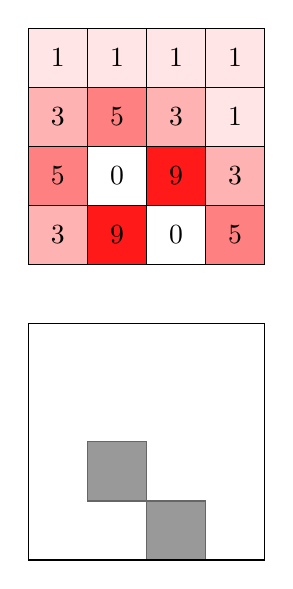
\begin{tikzpicture}[scale=0.75,line width=0.5pt]
    
    \filldraw[color=red!30] (0,0) rectangle (1,1);        
    \node at (0.5,0.5) {3};
    \filldraw[color=red!90] (1,0) rectangle (2,1); 
    \node at (1.5,0.5) {9};
    \filldraw[color=white] (2,0) rectangle (3,1); 
    \node at (2.5,0.5) {0};
    \filldraw[color=red!50] (3,0) rectangle (4,1); 
    \node at (3.5,0.5) {5};
    \filldraw[color=red!50] (0,1) rectangle (1,2); 
    \node at (0.5,1.5) {5};
    \filldraw[color=white] (1,1) rectangle (2,2); 
    \node at (1.5,1.5) {0};
    \filldraw[color=red!90] (2,1) rectangle (3,2); 
    \node at (2.5,1.5) {9};
    \filldraw[color=red!30] (3,1) rectangle (4,2); 
    \node at (3.5,1.5) {3};
    \filldraw[color=red!30] (0,2) rectangle (1,3); 
    \node at (0.5,2.5) {3};
    \filldraw[color=red!50] (1,2) rectangle (2,3); 
    \node at (1.5,2.5) {5};
    \filldraw[color=red!30] (2,2) rectangle (3,3); 
    \node at (2.5,2.5) {3};
    \filldraw[color=red!10] (3,2) rectangle (4,3); 
    \node at (3.5,2.5) {1};
    \filldraw[color=red!10] (0,3) rectangle (1,4); 
    \node at (0.5,3.5) {1};
    \filldraw[color=red!10] (1,3) rectangle (2,4); 
    \node at (1.5,3.5) {1};
    \filldraw[color=red!10] (2,3) rectangle (3,4); 
    \node at (2.5,3.5) {1};
    \filldraw[color=red!10] (3,3) rectangle (4,4); 
    \node at (3.5,3.5) {1};

    \draw (0,0) grid (4,4);
    
    \filldraw[color=black!60,fill=black!40] (1,-4) rectangle (2,-3); 
    \filldraw[color=black!60,fill=black!40] (2,-5) rectangle (3,-4); 
      
      \draw[black] (0,-5) -- (4,-5);
      \draw[black] (0,-5) -- (0,-1);
      \draw[black] (4,-1) -- (4,-5);
      \draw[black] (4,-1) -- (0,-1);
      
    \end{tikzpicture}
    \caption{Iteration 2: r = 9.21}
    %\label{fig:sfi2}
  \end{subfigure}
  \caption[First two iterations of {\tt GenerateMap}]{First two iterations of {\tt GenerateMap}, with $N$=4 and $D$=2. The top row shows the square matrix $m$ of potentials, and the bottom row shows the map itself.}
  %\label{fig:fig}
\end{figure}

\subsection{Map creation}

The system provides a tool for manually creating custom maps. This tool enables the creation of edge case maps for thorough testing of the algorithms.\\

\noindent
The Map Creation tool is accessed through the UI. The user is presented with a blank map of size $100 \times 100$, $200 \times 200$ or $400 \times 400$, and chooses a brush or eraser from a range of different sizes. The brush creates blocked cells wherever the user clicks and drags on the map, whereas the eraser creates free cells.\\

\noindent
The map size and brush size selections are implemented with radio buttons and drop-down combination boxes from {\em Java}'s {\em Swing} library. The click and drag capability is provided by a {\tt MouseMotionListener}, which calls a specific method any time the mouse's location changes whilst the mouse button is held.

\begin{figure}
\centering
  {\includegraphics[width=0.9\textwidth]{creationmode.png}}
  \caption[A map created with the Map Creation tool]{A map created with the Map Creation tool and solved by {\em A*} (orange) and {\em A* with post-smoothing} (red)} 
\end{figure}


\subsection{Loading a map}
Maps can be saved and loaded, which allows statistical analysis of the performance of the pathfinding algorithms to be performed on a fixed set of maps, and also allows the correctness of the pathfinding algorithms themselves to be thoroughly tested with a suite of edge case maps.\\

\noindent
The {\em Load} and {\em Save} buttons in the UI are {\tt JButton}s from the {\em Swing} library, which call a {\tt JFileChooser} when clicked (via the {\tt ActionListener} that is attached the the {\tt JButton}) which handles the creation of a load/save dialog box, and returns the file path of the map file that the user wishes to load/save.\\

\noindent
The map file is a platform independent binary representation of a {\tt Map} object, which is created when a map is saved by {\em serialising} the {\tt Map} object, and can be {\em deserialised} to load a map. {\em Serialisation}, which is the mechanism for creating a binary representation of an object, occurs when an object is passed as an argument to {\em Java}'s {\tt ObjectOutputStream} as long as the object's class implements the {\tt Serializable} marker interface, which is simply a way of telling the compiler that this class can be {\em serialised}.

\subsection{Start and goal point selection}
The selection of the start and goal points of the path works in a similar way to the map creation tool: radio buttons allow the user to specify which of the two points the user wishes to select, and a {\tt MouseListener} calls a method to record where on the map the user clicked.

\section{Graph generation}

This section introduces how graphs are implemented, and how both grid-based graphs and visibility graphs are generated from maps. The generation of visibility graphs requires the explanation of the {\em Line of Sight} algorithm, which is also used in the implementation of some of the pathfinding algorithms.\\

\subsection{Graphs}
A graph is implemented with a {\tt Graph} object, which is a set of {\tt Node} objects. Each {\tt Node} object has two floating-point instance variables to store its {\em g-value} and {\em f-value}, a {\tt Node} instance variable which points to its parent, and a {\tt Coordinate} object to store the location on the map that the node represents.\\

\noindent
As explained in the {\bfseries Preparation} chapter, every node expansion in the pathfinding algorithms sequentially iterates over the list of neighbours of that node. Therefore although edges are normally understood as a global property of a graph, the decision was made to implement edges as a {\tt LinkedList<Node>} instance variable of each {\tt Node} object, where the list contains the neighbours of that node. This allows fast and efficient access to the neighbour list of each node.\\

\subsection{Grid-based graph generation}
Section 2.1.2 presents a conceptual explanation of {\em discretisation}, which is the processes of generating a graph from a map. In this {\bfseries Implementation} chapter, the processes of generating a graph from a map is referred to as {\em graph generation}, to ensure that there is no confusion between the conceptual explanation (which was designed to assist the explanation of the algorithms within a graph-theoretic structure) and the actual implementation (which was designed to be computationally efficient). \\

\noindent{\bfseries Implementation}\\
\noindent
Starting with an empty set of nodes, the algorithm performs two loops:
\begin{enumerate}
\item for each location on the map that lies on the corner of a cell and is a {\em valid location}, a new node is inserted into the set  --- that is to say, $i$ is iterated over $0,1,\ldots,N-1$ and $j$ over $0,1,\ldots,N-1$, and a new {\tt Node} object with coordinate $(i,j)$ is inserted if $(i,j)$ is a {\em valid location}\footnote{A {\em valid location} in a map $M$ is defined in 2.1.1 as ``any location $(x,y) \in M$ that lies in a free cell or on the boundary of a free cell''.}.
\item for each node in the set, any of its eight neighbours are added to its neighbour list if:
  \begin{itemize}
  \item {\em diagonal neighbour} --- the cell that lies between the locations that the two nodes represent is not blocked;
  \item {\em horizontal or vertical neighbour} --- at least one of the cells that lie on either side of the location of the edge between those nodes is free.
  \end{itemize}
\end{enumerate}

\subsection{Visibility graph generation}
As discussed in the {\bfseries Preparation} chapter, this project focuses on the performance of pathfinding algorithms on grid-based graphs. However, the {\bfseries Evaluation} chapter will make use of visibility graphs, which are less space-efficient than grid-based graphs, but produce paths that are guaranteed to be optimal.\\

\noindent{\bfseries Implementation}\\
\noindent
Visibility graph generation is similar to that of grid-based graphs. Starting with an empty set of nodes, the algorithm performs two loops:
\begin{enumerate}
\item for each location on the map that lies on the corner of a cell, a new node is inserted into the set if exactly three of the surrounding four cells are free, or if the location is where either the {\em start} or {\em goal} of the path was selected by the user.
\item for each node in the set, any of the other nodes in the set are added to its neighbour list if a line of sight exists between the locations that the two nodes represent.
\end{enumerate}

\subsection{Line of Sight algorithm}
In the previous section, step 2 of the generation of visibility graphs requires an algorithm to test whether a line of sight exists between two locations. The {\bfseries Preparation} chapter also explained that many of the any-angle path finding algorithms require a line of sight algorithm.\\

\noindent
The {\em Line of Sight} algorithm is based on the pseudo-code in the publication of the {\em Theta*} algorithm \cite{Daniel10}, which itself is a derivative of {\em Bresenham's line drawing algorithm}\cite{Bresenham65}. {\em Bresenham's line drawing algorithm} determines which pixels in a raster display should be plotted in order to form a close approximation to a straight line between two given points $a$ and $b$, whereas the {\em Line of Sight} algorithm determines whether any of the cells that the straight line between two given points intersects are blocked. {\em Bresenham's line drawing algorithm} is a useful framework as it avoids any floating-point calculations when the endpoints of the line of sight are integers --- this has dual benefits:
\begin{itemize}
\item the algorithm is fast
\item the algorithm doesn't suffer from rounding errors inherent in floating-point calculations. 
\end{itemize}
\noindent
A notable alteration to {\em Bresenham's line drawing algorithm} is that while {\em Bresenham} draws one pixel per column (or one per row) of the raster display, the line of sight algorithm checks every cell that the line passes through, which may require multiple cells to be checked per column (or per row).\\

\noindent
For the purposes of clarity, the pseudocode presented in {\sc LineOfSight} assumes that the straight line between locations $a$ and $b$ is in `octant 1' - i.e. the angle that the line $ab$ makes with the horizontal is between $0^{o}$ and $45^{o}$.\\

\begin{algorithm}
  \SetAlgoLined\DontPrintSemicolon
  \SetKwFunction{los}{LineOfSight}
  \SetKwProg{myDef}{def}{}{}
  \myDef{\los($a$,$b$)}{
    \nl $ i \gets a.x$\;
    \nl $ j \gets a.y$\;
    \nl $ i_{b} \gets b.x$\;
    \nl $ j_{b} \gets b.y$\;
    \nl $ \Delta x \gets i_{b} - i$\;
    \nl $ \Delta y \gets j_{b} - j$\;
    \nl $ s \gets 0$\;
    \nl \While{$i \neq i_{b}$} {
      \nl $s \gets s + \Delta y$\;
      \nl \uIf{$i \geq \Delta x$} {
        \nl \uIf{$cell_{i,j}.isBlocked()$} {
          \nl \KwRet{$false$}\;
        }
        \nl $j \gets j+1$\;
        \nl $s \gets s - 1$\;
      }
      \nl \uIf{$s \neq 0 \land cell_{i,j}.isBlocked()$} {
        \nl \KwRet{$false$}\;
      }
      \nl \uIf{$\Delta y= 0 \land cell_{i,j}.isBlocked() \land cell_{i,j-1}.isBlocked()$} {
        \nl \KwRet{$false$}\;
      }
      \nl $i \gets i + 1$\;
    }
    \nl \KwRet{$true$}\;
  }
  \caption{{\sc LineOfSight}}
\end{algorithm} 

\section{Algorithm data}
The system uses a {\tt MapInstance} object to encapsulate the concept of a map --- with an associated {\em start} and {\em goal} location, the graph that represents that map, and the paths and path statistics calculated for that map by the pathfinding algorithms.\\

\noindent
Each {\tt MapInstance} has instance variables to store a {\tt Map} object, the grid-based {\tt Graph} and visibility {\tt Graph} objects that represent that map\footnote{{\tt Map} and {\tt Graph} objects have been introduced in subsections 3.1 and 3.2}, and a list of {\tt AlgorithmData} objects to store the paths and path statistics for the any pathfinding algorithms that have been run on this map.\\

\noindent
There is a concrete class for each pathfinding algorithm that inherits from the abstract class {\tt AlgorithmData} --- which  has an {\em enum} type denoting which pathfinding algorithm the object is holding data for, a public method {\tt go()} which is called to run the pathfinding algorithm, and getter methods which return statistical data about the path found, such as:

\begin{description}
\item {\bf Path exists}\\ \hfill
whether or not the pathfinding algorithm found a valid path between the {\em start} and {\em goal};
\item {\bf Path length}\\ \hfill
the path length;
\item {\bf Cumulative path angle}\\ \hfill
the path angle-sum;
\item {\bf Graph calculation time}\\ \hfill
the duration between the call to {\tt generateGraph()} and {\tt generateGraph()} returning, calculated with {\tt System.nanoTime()};
\item {\bf Path calculation time}\\ \hfill
the duration between the call to {\tt getPath()} and {\tt getPath()} returning, calculated with {\tt System.nanoTime()};
\item {\bf Number of nodes expanded}\\ \hfill
the number of nodes that were expanded by the pathfinding algorithm.
\end{description}

\begin{figure}
\centering
\begin{tikzpicture} [scale=1.2]
\umlsimpleclass{MapInstance} 
\umlsimpleclass[x=-4,y=-2.5]{Map} 
\umlsimpleclass[x=0,y=-2.5]{Graph}
\umlsimpleclass[x=4,y=-2.5,type=abstract]{AlgorithmData}
\umlsimpleclass[x=-4,y=-5]{Cell} 
\umlsimpleclass[x=0,y=-5]{Node} 
\umlsimpleclass[x=-2,y=-7.5]{Coordinate} 
%\umlclass[x=4,y=-3,type=abstract]{AlgorithmData}{- distance : $double$ \\ - angle : $double$ \\ - path : $List<Coordinate>$ \\ ...}{+ go() : void \\ \# getPath($graph : Graph$) : $Node$ \\ ...} 
\umlHVuniassoc[arg1=1, pos1=0.2, align1=left,arg2=1, pos2=2, align2=right]{MapInstance}{Map}
\umluniassoc[arg1=1, pos1=0.3, align1=right,arg2=2, pos2=1, align2=right]{MapInstance}{Graph}
\umlHVuniassoc[arg1=1, pos1=0.2, align1=right, arg2=7, pos2=2, align2=right]{MapInstance}{AlgorithmData}
\umluniassoc[arg1=1, pos1=0.3, align1=right,arg2=*, pos2=1, align2=right]{Map}{Cell}
\umluniassoc[arg1=1, pos1=0.3, align1=right,arg2=*, pos2=1, align2=right]{Graph}{Node}
%\umluniassoc[mult1=1,pos1=0,mult2=*,pos2=1, angle1=-45, angle2=-135, loopsize=3cm]{Node}{Node}
\umluniassoc[mult1=1,pos1=0.1,mult2=*,pos2=0.9, angle1=45, angle2=-45, loopsize=3cm]{Node}{Node}
\umlVHuniassoc[arg1=1, pos1=0.2, align1=left,arg2=1, pos2=2, align2=right]{Cell}{Coordinate}
\umlVHuniassoc[arg1=1, pos1=0.2, align1=right,arg2=1, pos2=2, align2=left]{Node}{Coordinate}
\end{tikzpicture}
\caption{Composition of {\tt MapInstance}}
\end{figure}

\section{Pathfinding algorithms}
To emphasise the close relationships between the algorithms and allow for maximum code re-use, the concrete classes that implement the algorithms are arranged in a hierarchy that closely reflects the relationship between the algorithms. However, despite {\em Block A*} having a similar basic structure to {\em A*}, a compromise had to be made by having {\em Block A*} inheriting directly from {\em AlgorithmData} as the actual implementation of {\em Block A*} is too different from {\em A*} to allow any meaningful inheritance in the code.\\

\noindent
The inheritance caused by the hierarchy also ensures that any performance differences between algorithms is due to the different nature of each algorithm and not different implementations of similar concepts.\\

\begin{figure}
\centering
\begin{tikzpicture} [scale=1]
\umlemptyclass[type=abstract]{AlgorithmData}
\umlemptyclass[x=-2,y=-3]{Dijkstra}
\umlemptyclass[x=2,y=-3]{BlockAStar}
\umlemptyclass[x=-2,y=-6]{AStar}
\umlemptyclass[x=-2,y=-9]{AStarSmoothed}
\umlemptyclass[x=2,y=-9]{ThetaStar}
\umlemptyclass[x=2,y=-12]{LazyThetaStar}
\umlVHVreal{Dijkstra}{AlgorithmData}
\umlVHVreal{BlockAStar}{AlgorithmData}
\umlVHVinherit{AStar}{Dijkstra}
\umlVHVinherit{AStarSmoothed}{AStar}
\umlVHVinherit{ThetaStar}{AStar}
\umlVHVinherit{LazyThetaStar}{ThetaStar}

\end{tikzpicture}
\caption{Inheritance structure of algorithm implementations}
\end{figure}

\noindent
The remainder of this section explains the decisions and strategies employed when implementing the pathfinding algorithms.

\subsection{Dijkstra's shortest paths}
The implementation is based on the pseudo-code seen in Algorithm 1 in the {\bfseries Preparation} chapter. By using the {\tt Graph} and {\tt Node} classes introduced in subsection 3.2.1, the translation from pseudo-code to {\em Java} code is transparent. The notable implementation decisions are detailed below:
\begin{description}
  \item {\bf Closed set}\\ \hfill
  the only two operations on the {\tt closedSet} are adding and checking for membership. Therefore, a {\tt HashSet} is used for its average case O(1) insertion and search speed.
  \item {\bf Distance calculations}\\ \hfill
  since there are a known set of possible node locations in a map of a given size, costly square root calculations are avoided by using a pre-calculated lookup table for finding the Euclidean distance between coordinates. This is also employed by {\em A*} and its derivatives when calculating $h-value$s.
  \item {\bf Extensibility} \\ \hfill
  to allow the inheritance hierarchy shown in Figure 3.7, {\tt Dijkstra} (i.e. the implementation of {\em Dijkstra}) includes a call to two methods which are required by algorithms that inherit from {\tt Dijkstra}, but are not actually needed by {\tt Dijkstra} itself. The first is {\tt initialise(Node n)} which is called when a node {\tt n} is popped from the {\tt openSet} (which is used by {\em Lazy Theta*}), and the second is a {\tt postProcessing(Node n)} step before the goal node is returned (which is used by {\em A* with post-processing}). In {\tt Dijkstra}  these methods have empty bodies.
  \end{description}

\subsection{A*}
{\tt AStar} inherits from {\tt Dijkstra}, and only overrides the {\tt updateCost()} method in accordance with the pseudo-code in Algorithm 2.

\subsection{A* with post-smoothing}

{\tt AStarPostSmoothing} inherits from {\tt AStar}, and implements the post-smoothing by overriding the {\tt postProcessing()} method which had an empty body in {\tt Dijkstra} and {\tt AStar}. As per the majority of the implementations of {\tt Dijkstra} and {\tt AStar}, the code required for the implementation of {\tt AStarPostSmoothing} is a transparent translation of the pseudo-code presented in the {\bfseries Preparation} chapter.\\

\subsection {Theta* and Lazy Theta*}

The implementations are based on the pseudo-code in Algorithm 4 and Algorithm 5: 
\begin{description}
\item{\bfseries Theta*}\\ \hfill inherits from {\tt AStar}, and only overrides the {\tt updateCost()} method. {\tt ThetaStar} uses the implementation of the {\em Line of Sight} algorithm introduced in subsection 3.2.4.
\item {\bfseries Lazy Theta*}\\ \hfill inherits from {\tt ThetaStar}, and overrides the {\tt initialiseNode()} and {\tt updateCost()} methods. Note that {\tt LazyThetaStar} is the only class to implement {\tt initialiseNode()}.
\end{description}

\subsection {Block A*}
The implementation of {\em Block A*} is by far the most complex, and hence interesting, of all of the pathfinding algorithms ---partly because {\em Block A*} is the most intricate of the pathfinding algorithms, and partly because {\em Yap et al.}'s paper left large parts of the implementation details unspecified. This provides an opportunity to investigate some different implementation strategies which are described in this section and then compared for efficiency and performance in the {\bfseries Evaluation} chapter.\\

\noindent{\bfseries LDDB --- overview}\\
\noindent
As a reminder for the reader, subsection 2.2.8 defines a Local Distance Database $LDDB$ for block size $N \times N$ as ``$LDDB_{N}$ , a pre-computed database that holds the path length and inflection points of the optimum paths between all {\em ingress-egress} pairs of locations $(a,b)$-$(c,d)$ for all map configurations $M$ of size $N \times N$, where $a,b,c,d \in \mathbb{Z}$ and $(a,b)$-$(c,d)$ lies on the boundary of $M$''. Since each block expansion requires the knowledge of shortest paths between {\em ingress-egress} pairs of coordinates that lie on the boundary of the block, {\em Block A*} speeds up the expansion of blocks by using the $LDDB$ to avoid explicitly calculating the paths.\\

\noindent
Since there is no publicly available library containing $LDDB$s for {\em Block A*}, the first challenge was to create the $LDDB$s. Although {\em Block A*} only uses a $LDDB$ of a single block size, multiple $LDDB$s are required for this project so that performance tradeoffs between $LDDB$s of different block sizes can be investigated. By definition, an $LDDB$ is applicable to any map, so the $LDDB$s only need to be calculated once for each block size\footnote{As explained later in this section, the three block sizes that are investigated in this project are $2 \times 2$, $3 \times 3$ and $4 \times 4$, so only three $LDDB$s were required: $LDDB_{2}$, $LDDB_{3}$ and $LDDB_{4}$.}. A method is required to create the $LDDB$s automatically, since for blocks of size {$N \times N$} there are $2^{N^{2}}$ possible blocks each with $4.N.4.(N-1)$ pairs of $ingress$ and $egress$ coordinates, which gives over 12 million optimal path calculations for a block size of $4 \times 4$.\\

\noindent
Each $LDDB_{N}$ contains:\\
(1) \indent for every possible map of size $N \times N$\\
(2) \indent \indent for every possible $ingress-egress$ coordinate pair\\
(3a) \indent \indent \indent the shortest path between that pair, and\\
(3b) \indent \indent \indent a list containing every intermediate coordinate on that path.\\

\noindent
The above steps were implemented as follows:
\begin{description}
\item (1) ``every possible map of size $N \times N$'' is enumerated by converting each integer from $0$ to $2^{N^{2}}-1$ to the corresponding map representation --- since a map of size $N \times N$ can be represented as a binary integer of $N^{2}$ bits where each bit represents a cell in the map, and that cell is free if the corresponding bit is 0 and is blocked if the bit is 1. See Figure 3.8.
\item (2) ``every possible $ingress-egress$ coordinate pair'' is enumerated by looping over every possible $egress$ coordinate for every possible $ingress$ coordinate, where the possible $ingress$ and $egress$ coordinates are the locations of all nodes that lie on the boundary of a block --- that is to say, all nodes whose coordinates are $(i,j)$, where $[(i=0 \lor i=N) \land (0\leq j \leq N)] \lor [(0\leq i \leq N) \land (j-0 \lor j=N)]$.
\item (3) the shortest path through a map between a given $ingress-egress$ coordinate pair is found by converting the map to a visibility graph and then finding the optimal path through it with {\em A*} (with $ingress = start$ and $egress=goal$). The length required by (3a) is the final value of $n_{goal}.g$, and the list of intermediate coordinates required by (3b) is found by removing the coordinates of $start$ and $goal$ from the list of coordinates in the path returned by {\em A*}.
\end{description}

\begin{figure}
    \centering
    \begin{subfigure}{.18\textwidth}
    \centering
    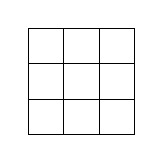
\begin{tikzpicture}[scale=0.45,line width=0.5pt]
    \draw[color=black] (0,0) grid (3,3);
    \end{tikzpicture}
    \caption{0}
    \end{subfigure}
    \begin{subfigure}{.18\textwidth}
    \centering
    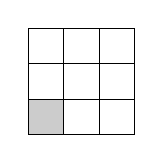
\begin{tikzpicture}[scale=0.45,line width=0.5pt]
    \filldraw[black!20] (0,0) rectangle (1,1);
    \draw[color=black] (0,0) grid (3,3);
    \end{tikzpicture}
    \caption{1}
    \end{subfigure}
     \begin{subfigure}{.18\textwidth}
     \centering
    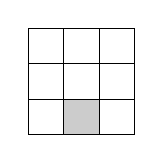
\begin{tikzpicture}[scale=0.45,line width=0.5pt]
    \filldraw[black!20] (1,0) rectangle (2,1);
    \draw[color=black] (0,0) grid (3,3);
    \end{tikzpicture}
    \caption{2}
    \end{subfigure}
    \begin{subfigure}{.18\textwidth}
    \centering
    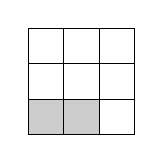
\begin{tikzpicture}[scale=0.45,line width=0.5pt]
    \filldraw[black!20] (0,0) rectangle (2,1);
    \draw[color=black] (0,0) grid (3,3);
    \end{tikzpicture}
    \caption{3}
    \end{subfigure}
    \begin{subfigure}{.18\textwidth}
    \centering
    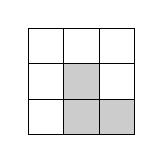
\begin{tikzpicture}[scale=0.45,line width=0.5pt]
    \filldraw[black!20] (1,0) rectangle (3,1);
    \filldraw[black!20] (1,0) rectangle (2,2);
    \draw[color=black] (0,0) grid (3,3);
    \end{tikzpicture}
    \caption{22}
    \end{subfigure}
  \caption{Integer encoding scheme of maps}
  %\label{fig:fig}
\end{figure}

\noindent{\bfseries LDDB --- uncompressed implementation}\\
\noindent
It is necessary to store the paths and intermediates nodes calculated in steps (3a) and (3b) in a database structure that is compact in memory (so that as much of it as possible can fit into cache) and fast to load and query. Since these constraints are fundamental to the operation of the algorithm, any library or 3\textsuperscript{rd} party database implementation can not be guaranteed to be sufficiently specialised for the task, so a custom database is implemented using arrays and hash tables to ensure optimal performance and minimum space wastage.\\

\noindent
Queries to the $LDDB$ require arguments that describe:
\begin{description} 
\item{the configuration of the block:\footnote{I.e. the configuration of the sub-map that the block represents}}\\
the simple bitwise scheme shown in Figure 3.8 is used to describe the configuration of a block, and the 32 bits of the {\em Java} {\tt int} primitive is sufficient to encode all possible block configurations of all the block sizes $N$ that are considered in this project\footnote{The reasons for this are explained in the {\bfseries Evaluation} chapter.}: $N=2, 3, 4$. This encoding scheme has dual benefits:
\begin{itemize}
\item the encoded integers are a small (32 bit) value that can be cheaply stored within the {\tt Block} object itself;
\item since these encoded integers form a sequential sequence, they allow the $LDDB_{N}$ to be implemented as an array of size $2^{N^{2}}-1$ which can be indexed by using the encoded integer. This is advantageous as arrays are the most efficient storage format in terms of space and random-access time, which is required by this database.
\end{itemize}


\item{an $ingress-egress$ coordinate pair}:\\
the $ingress-egress$ coordinate pairs do not fill a sequential space so it would be spatially inefficient to have these coordinate pairs indexing into an array as the array would be sparse. Therefore, the $ingress-egress$ coordinate pairs index into a hash table, which provides relatively fast random access and space-efficiency for a non-sequential, non-uniform key space.\\

\end{description}

\noindent
Query results from the $LDDB$ are either the length of the shortest path between those nodes, i.e. (3a), or a list of the intermediate coordinates on the shortest path between the $ingress$ and the $egress$, i.e. (3b).\\

\noindent
Therefore the underlying implementation of the uncompressed implementation database is an array of {\tt  HashMaps} - one {\tt HashMap} per block configuration, with the array indexed by the encoded integer that represents the block, and each {\tt HashMap} mapping a key (a {\tt Pair} of $ingress-egress$ {\tt Coordinate}s) to a value (a {\tt Pair} consisting of the length (as a {\tt double}) of the shortest path between the $ingress$ and the $egress$, and an {\tt ArrayList} of the intermediate {\tt Coordinate}s on that path).\\

\begin{figure}
    \centering
    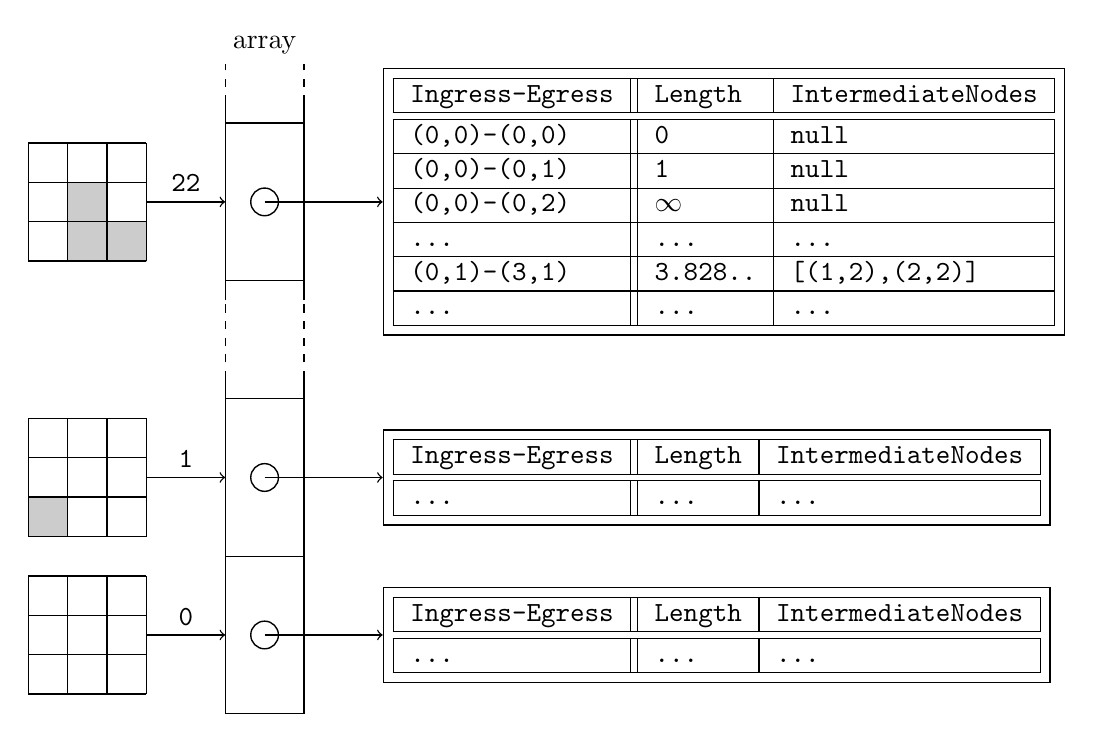
\begin{tikzpicture}[scale=0.5,line width=0.5pt]
    
    \filldraw[black!20] (0,4) rectangle (1,5);
    
    \filldraw[black!20] (1,11) rectangle (2,13);
    \filldraw[black!20] (2,11) rectangle (3,12);
    
      \draw (0,0) grid (3,3);
      \draw (0,4) grid (3,7);
      \draw (0,11) grid (3,14);
      
      \draw (5,-0.5) -- (5,8);
      \draw[dashed] (5,8) -- (5,10);
      \draw(5,10) -- (5,15);
      \draw[dashed] (5,15) -- (5,16);
      \draw (7,-0.5) -- (7,8);
      \draw[dashed] (7,8) -- (7,10);
      \draw(7,10) -- (7,15);
      \draw[dashed] (7,15) -- (7,16);
      
      \draw (5,-0.5) -- (7,-0.5);
      \draw (5,3.5) -- (7,3.5);
      \draw (5,7.5) -- (7,7.5);
      \draw (5,10.5) -- (7,10.5);
      \draw (5,14.5) -- (7,14.5);
      
      \draw[->] (3,1.5) -- (5,1.5);
      \draw[->] (3,5.5) -- (5,5.5);
      \draw[->] (3,12.5) -- (5,12.5);
      
      \node[above] at (4,1.5) {\tt 0};
      \node[above] at (4,5.5) {\tt 1};
      \node[above] at (4,12.5) {\tt 22};
      \node[above] at (6,16) {array};
      
      \draw[->] (6,1.5) -- (9,1.5);   
      \draw (6,1.5) circle (10pt);
      \node[right,draw=black,shape=rectangle] at (9,1.5) (1) {
      \begin{tabular}{| l || l | l |}
    \hline
    {\tt Ingress-Egress} & {\tt Length} & {\tt IntermediateNodes}  \\ \hline \hline
    {\tt ...}  & {\tt ...} & {\tt ...} \\ \hline
    \end{tabular}};
      \draw[->] (6,5.5) -- (9,5.5);
      \draw (6,5.5) circle (10pt);
      \node[right,draw=black,shape=rectangle] at (9,5.5) (1) {
            \begin{tabular}{| l || l | l |}
    \hline
    {\tt Ingress-Egress} & {\tt Length} & {\tt IntermediateNodes}  \\ \hline \hline
    {\tt ...}  & {\tt ...} & {\tt ...} \\ \hline
    \end{tabular}};
      \draw[->] (6,12.5) -- (9,12.5);
      \draw (6,12.5) circle (10pt);
      \node[right,draw=black,shape=rectangle] at (9,12.5) (1) {
    \begin{tabular}{| l || l | l |}
    \hline
    {\tt Ingress-Egress} & {\tt Length} & {\tt IntermediateNodes}  \\ \hline \hline
    {\tt (0,0)-(0,0)}  & {\tt 0} & {\tt null} \\ \hline
    {\tt (0,0)-(0,1)}  & {\tt 1} & {\tt null} \\ \hline
    {\tt (0,0)-(0,2)}  & {\tt $\infty$} & {\tt null} \\ \hline
    {\tt ...}  & {\tt ...} & {\tt ...} \\ \hline
    {\tt (0,1)-(3,1)}  & {\tt 3.828..} & {\tt [(1,2),(2,2)]} \\ \hline
    {\tt ...}  & {\tt ...} & {\tt ...} \\ \hline
\end{tabular}};
      
    \end{tikzpicture}
  \caption[Extract of the uncompressed implementation of $LDDB_{3}$]{Extract of the uncompressed implementation of $LDDB_{3}$, detailing part of the {\tt HashTable} for the block configuration which has an encoded integer representation of 22}
  %\label{fig:fig}
\end{figure}

\noindent
The next three subsections build upon this uncompressed implementation by describing some different compression techniques that were devised for the $LDDB$, and three different strategies for obtaining the edge weights in the special case blocks. All of the different resulting forms of $LDDB$ involve tradeoffs between space and time which are analysed in the {\bfseries Evaluation} chapter.\\

\noindent{\bfseries LDDB --- bitwise-compressed implementation}\\
\noindent
An implementation was devised that makes use of a further bitwise encoding scheme to encode {\tt PairOfCoords} and {\tt List<Coordinate>}:
\begin{enumerate}
\item each {\tt Pair} of ingress-egress {\tt Coordinate}s can be represented with a unique integer in a {\tt byte}'s worth of space. An efficient hash function was devised to convert from a {\tt PairOfCoordinate} object to this encoded byte representation that uses bit shifting to represent each coordinate with 6 bits, since the range of $x$ and $y$ in each {\tt Coordinate} in a sub-map of size up to {$N=4$} is 0-4 which is representable with 3 bits. See Figure 3.10.
\item the {\tt List} of intermediate {\tt Coordinate}s can be represented by a unique code that fits into the 32 bits of an integer by using the scheme in the above, since: the maximum\footnote{Obtained by querying the length of the intermediate coordinate list for every entry in the uncompressed $LDDB_{4}$.} number of intermediate nodes on a shortest path in a sub-map of size up to {$N=4$} is 4, is a maximum total of 4*6 = 24 bits. The encoding scheme is identical to the hash function for the {\tt Pair} of ingress-egress {\tt Coordinate}s.
\end{enumerate}

\noindent
Furthermore, the length of a path (stored as a 32 bit {\tt float}) and the integer that represents the intermediate coordinates can then be compressed into one 64 bit {\tt long} integer (which is the native register size of most modern architectures), to produce one 64 bit $LDDB$ entry per $ingress-egress$ pair.\\

\begin{figure}
\begin{lstlisting}
private int getCode(Coordinate c1, Coordinate c2) {
		int code = 0;
		code = code | c1.getX();
		code = code << 3;
		code = code | c1.getY();
		code = code << 3;
		code = code | c2.getX();
		code = code << 3;
		code = code | c2.getY();
		return code;	
	}
\end{lstlisting}
\caption{Encoding scheme for {\tt PairOfCoords} in the bitwise-compressed {\em LDDB}}
\end{figure}

\noindent{\bfseries LDDB --- geometrically-compressed implementation}\\
\noindent
The bitwise-compressed implementation of the database uses bitwise encoding schemes to compress the database. Further approaches to compression are possible by taking advantage of the symmetry between different block configurations and $ingress-egress$ pairs:
\begin{enumerate}
\item some block configurations are 90$^{\circ}$,  180$^{\circ}$ or 270$^{\circ}$ rotations of other block configurations.
\item the shortest path between an $ingress-egress$ pair $a$ and $b$ is the reverse of the shortest path between an $ingress-egress$ pair $b$ and $a$. 
\end{enumerate}

These two properties leverage the redundancy in the compressed database as described below:
\begin{enumerate}
\item The data for only one of the four rotations of block configuration needs to be stored in the database. A simple policy is used to determine which of the rotations is stored --- the rotation with the smallest encoded integer representation (as introduced for the uncompressed implementation of the $LDDB$) is the one that is stored. Note that if the block configuration does need to be rotated in the query, then the intermediate nodes in the query result will need to be rotated by the same amount in the opposite direction. 
\item The data for only one of the two `reflection' pairs of $ingress-egress$ coordinates $a,b$ and $b,a$ needs to be stored in the database. A simple policy is used to determine which one of these two pairs is stored --- if $a.y < b.y$ or $(a.y = b.y) \land (a.x \leq b.y)$ then the pair will be found as $a,b$ in the database, otherwise they are found as $b,a$. Note that if the $ingress-egress$ pair needs to be reversed in the query, then the intermediate nodes in the query result will also need to be reversed. 
\end{enumerate}

\noindent
Figure 3.11 gives an annotated explanation of a query to a bitwise \& geometrically compressed $LDDB$ --- see A.6 for an extended explanation. In the actual implementation, some of this work is saved by storing the rotation value (calculated in step (b)) in an instance variable of each {\tt Block}. Furthermore, the coordinate rotations (calculated in steps (b) and (g)) take only one of four forms (since the block have rotational symmetry of up to four), hence the pre-rotation to post-rotation (and vice versa) coordinate mappings are obtained by querying one of four small pre-calculated tables stored as {\tt static} variables of the {\tt Block} class.\\

\begin{figure}
    \centering
    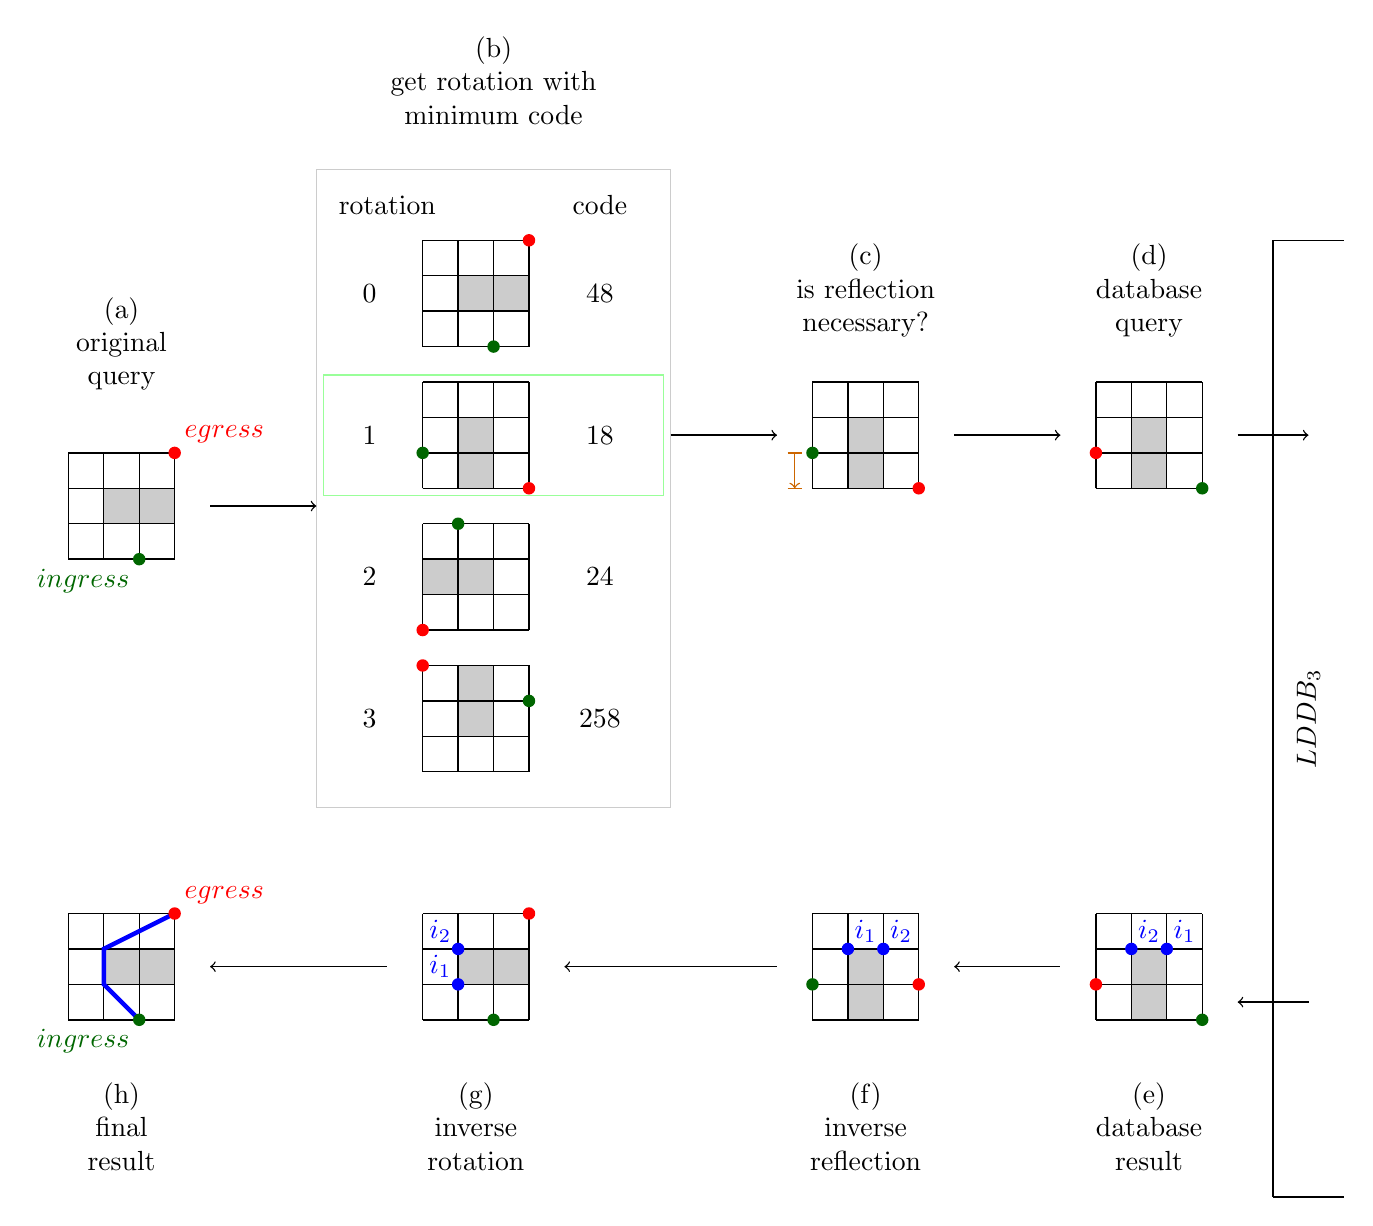
\begin{tikzpicture}[scale=0.45,line width=0.5pt]
    
    %input
    \filldraw[black!20] (-9,7) rectangle (-7,8);
    \draw (-10,6) grid (-7,9);
    \fill[black!60!green] (-8,6) circle (5pt);
    \node[below left, black!60!green] at (-8,6) {$ingress$};
    \fill[red] (-7,9) circle (5pt);
    \node[above right, red] at (-7,9) {$egress$};
    \node[above,align=center] at (-8.5,10.5) {(a) \\ original \\ query};
    
    %rotations
    \draw[black!20] (-3,-1) rectangle (7,17);
    \draw[green!40] (-2.8,7.8) rectangle (6.8,11.2);
    
    \filldraw[black!20] (1,13) rectangle (3,14);
    \draw (0,12) grid (3,15);
    \fill[black!60!green] (2,12) circle (5pt);
    \fill[red] (3,15) circle (5pt);
        
    \filldraw[black!20] (1,8) rectangle (2,10);
    \draw (0,8) grid (3,11);
    \fill[black!60!green] (0,9) circle (5pt);
    \fill[red] (3,8) circle (5pt);
        
    \filldraw[black!20] (0,5) rectangle (2,6);
    \draw (0,4) grid (3,7);
    \fill[black!60!green] (1,7) circle (5pt);
    \fill[red] (0,4) circle (5pt);
    
    \filldraw[black!20] (1,1) rectangle (2,3);
    \draw (0,0) grid (3,3);
    \fill[black!60!green] (3,2) circle (5pt);
    \fill[red] (0,3) circle (5pt);
    
    \draw[->] (-6,7.5) -- (-3,7.5);
    
    \node at (-1,16) {rotation};	\node at (5,16) {code};
    \node at (-1.5,13.5) {0};		\node at (5,13.5) {48};
    \node at (-1.5,9.5) {1};		\node at (5,9.5) {18};
    \node at (-1.5,5.5) {2};		\node at (5,5.5) {24};
    \node at (-1.5,1.5) {3};		\node at (5,1.5) {258};
    
    \draw[->] (7,9.5) -- (10,9.5);
    \node[above,align=center]  at (2,18) {(b) \\ get rotation with \\ minimum code};
   
   %angle check
    \filldraw[black!20] (12,8) rectangle (13,10);
    \draw (11,8) grid (14,11);
    \draw[orange!80!black, ->] (10.5,9) -- (10.5,8);
    \draw[orange!80!black] (10.3,9) -- (10.7,9);
    \draw[orange!80!black] (10.3,8) -- (10.7,8);
    \fill[black!60!green] (11,9) circle (5pt);
    \fill[red] (14,8) circle (5pt);
    \node[above,align=center]  at (12.5,12) {(c) \\ is reflection \\ necessary?};
    
    \draw[->] (15,9.5) -- (18,9.5);
    
    %DB input
    \filldraw[black!20] (20,8) rectangle (21,10);
    \draw (19,8) grid (22,11);
    \fill[red] (19,9) circle (5pt);
    \fill[black!60!green] (22,8) circle (5pt);
    \node[above,align=center]  at (20.5,12) {(d) \\ database \\ query};
    
    \draw[->] (23,9.5) -- (25,9.5);
    \draw (24,15) -- (26,15);
    \draw (24,-12) -- (26,-12);
    \draw (24,-12) -- (24,15);
    \node[rotate=90] at (25,1.5) {$LDDB_{3}$};
        
    \draw[<-] (23,-6.5) -- (25,-6.5);
    
    %DB output
    \filldraw[black!20] (20,-7) rectangle (21,-5);
    \draw (19,-7) grid (22,-4);
    \fill[red] (19,-6) circle (5pt);
    \fill[black!60!green] (22,-7) circle (5pt);
    \fill[blue] (21,-5) circle (5pt);
    \node[blue] at (21.5,-4.5) {$i_{1}$};
    \fill[blue] (20,-5) circle (5pt);
    \node[blue] at (20.5,-4.5) {$i_{2}$};
    \node[below,align=center]  at (20.5,-8.5) {(e) \\ database \\ result};
    
    \draw[<-] (15,-5.5) -- (18,-5.5);
    
    %flipped
    \filldraw[black!20] (12,-7) rectangle (13,-5);
    \draw (11,-7) grid (14,-4);
    \fill[black!60!green] (11,-6) circle (5pt);
    \fill[red] (14,-6) circle (5pt);
    \fill[blue] (12,-5) circle (5pt);
    \node[blue] at (12.5,-4.5) {$i_{1}$};
    \fill[blue] (13,-5) circle (5pt);
    \node[blue] at (13.5,-4.5) {$i_{2}$};
    \node[below,align=center]  at (12.5,-8.5) {(f) \\ inverse \\ reflection};
    
    \draw[<-] (4,-5.5) -- (10,-5.5);
    
    %rotated
    \filldraw[black!20] (1,-6) rectangle (3,-5);
    \draw (0,-7) grid (3,-4);
    \fill[black!60!green] (2,-7) circle (5pt);
    \fill[red] (3,-4) circle (5pt);
    \fill[blue] (1,-6) circle (5pt);
    \node[blue] at (0.5,-5.5) {$i_{1}$};
    \fill[blue] (1,-5) circle (5pt);
    \node[blue] at (0.5,-4.5) {$i_{2}$};
    \node[below,align=center]  at (1.5,-8.5) {(g) \\ inverse \\ rotation};
    
    \draw[<-] (-6,-5.5) -- (-1,-5.5);
    
     \filldraw[black!20] (-9,-6) rectangle (-7,-5);
    \draw (-10,-7) grid (-7,-4);
    \draw[blue,ultra thick] (-8,-7) -- (-9,-6) -- (-9,-5) -- (-7,-4);
    \fill[black!60!green] (-8,-7) circle (5pt);
    \node[below left, black!60!green] at (-8,-7) {$ingress$};
    %\fill[blue] (-9,-7) circle (5pt);
    %\fill[blue] (-9,-6) circle (5pt);
    \fill[red] (-7,-4) circle (5pt);
    \node[above right, red] at (-7,-4) {$egress$};
    \node[below,align=center]  at (-8.5,-8.5) {(h) \\ final \\ result};
    
    \end{tikzpicture}
  \caption{Annotated explanation of a bitwise \& geometrically-compressed $LDDB_{3}$ query}
\end{figure}

\noindent
{\bf Special case blocks}\\

\noindent
As explained in 2.2.8, the edge weights for $block_{start}$ and $block_{goal}$ may not be present in the $LDDB$ because the $LDDB$ only contains data for paths between $ingress$ and $egress$ coordinates (which lie on the boundaries of blocks), yet $start$ and $goal$ are not guaranteed to lie on the boundary of a block. Therefore, alternative methods must be used to obtain the edge weights for $block_{start}$ and $block_{goal}$:
\begin{description}
\item {\em Option 1:} {\bfseries compute the edge weights at runtime}, by using a similar method to that which is used to compute the shortest paths contained in the $LDDB$ --- i.e. by generating a visibility graph to represent the sub-map that $block_{start}$ represents, and using {\em A*} to find the shortest path between $n_{start}$ and all boundary nodes of $block_{start}$ (and then similarly for $block_{goal}$). In the exceptional case that $block_{start} = block_{goal}$, this method can be slightly modified to return the shortest path directly. 
\item {\em Option 2:} {\bfseries extend the LDDB} so that it also includes data for all possible edges in $block_{start}$ and $block_{goal}$. The unextended $LDDB$ (regardless of whether of not it is bitwise or geometrically compressed) contains details of shortest paths from {\em any boundary} node to {\em any boundary} node in a block, so there are two possibilities for extension:
  \begin{description}
  \item{\em (a)} {\bf semi-extended $LDDB$} contains details of shortest paths from {\em any} node to {\em any boundary} node in a block. This $LDDB$ will have all data required by {\em Block A*} for all blocks, except for in the exceptional case that $block_{start} = block_{goal}$, in which case a visibility graph of the block must be calculated and solved with {\em A*} as in {\em Option 1}.
  \item{\em (b)} {\bf fully-extended $LDDB$} contains details of shortest paths from {\em any} node to {\em any} node in a block. This $LDDB$ will have all data required by {\em Block A*} for all blocks.
  \end{description} 
\end{description}

\begin{figure}
\centering
\begin{tikzpicture} [scale=0.7]
\umlemptyclass{BlockAStar}
\umlemptyclass[x=-4,y=-4]{BlockAStar\_SemiExtended}
\umlemptyclass[x=-8,y=-8]{BlockAStar\_FullyExtended}
\umlemptyclass[x=4,y=-8,type=interface]{LDDB}
\umlemptyclass[x=-8,y=-13]{LDDB\_Uncompressed}
\umlemptyclass[x=-2,y=-13]{LDDB\_Bitwise}
\umlemptyclass[x=4,y=-13]{LDDB\_Geometric}
\umlemptyclass[x=10,y=-13]{LDDB\_BitAndGeo}
\umlemptyclass[x=-5,y=-18]{PoC\_Uncompressed}
\umlemptyclass[x=1,y=-18]{PoC\_Bitwise}
\umlemptyclass[x=7,y=-18]{RotationTable}
\umlemptyclass[x=-2,y=-22,type=abstract]{PairOfCoordinates}

\umlVHVinherit{BlockAStar\_SemiExtended}{BlockAStar}
\umlVHVinherit{BlockAStar\_FullyExtended}{BlockAStar\_SemiExtended}
\umlVHuniassoc{LDDB}{BlockAStar}
\umlVHVimpl{LDDB\_Uncompressed}{LDDB}
\umlVHVimpl{LDDB\_Bitwise}{LDDB}
\umlVHVimpl{LDDB\_Geometric}{LDDB}
\umlVHVimpl{LDDB\_BitAndGeo}{LDDB}
\umluniassoc[geometry=|-|, weight=0.65]{PoC\_Uncompressed}{LDDB\_Uncompressed}
\umluniassoc[geometry=|-|, weight=0.65]{PoC\_Uncompressed}{LDDB\_Geometric}
\umluniassoc[geometry=|-|, weight=0.5]{PoC\_Bitwise}{LDDB\_Bitwise}
\umluniassoc[geometry=|-|, weight=0.5]{PoC\_Bitwise}{LDDB\_BitAndGeo}
\umluniassoc[geometry=|-|, weight=0.35]{RotationTable}{LDDB\_Bitwise}
\umluniassoc[geometry=|-|, weight=0.35]{RotationTable}{LDDB\_BitAndGeo}
\umlVHVimpl{PoC\_Uncompressed}{PairOfCoordinates}
\umlVHVimpl{PoC\_Bitwise}{PairOfCoordinates}

\end{tikzpicture}
\caption{Class structure of different implementations of {\em Block A*}}
\end{figure}

\noindent{\bfseries Algorithm} \\
\noindent
Having carefully set up the problem in the {\bfseries Preparation} chapter, the core part of the implementation of the algorithm is a transparent translation of the pseudo-code in Algorithm 6 using similar design choices to the other pathfinding algorithms. However, the pseudo-code does not specify the implementation of the creation of {\tt Init}, {\tt TraceBack} or the creation of blocks, which also require the application of many of many of the techniques and design choices seen in the other algorithms, but to a far more complicated level. The {\tt BlockAStar} class itself is over 400 lines of Java (excluding comments), which doesn't include the implementation of blocks or the creation and decoding of the various $LDDB$ implementations.\\

\noindent{\bfseries Traceback}\\
\noindent
Finally the traceback stage, which is unspecified in {\em Yap et al.}'s paper and the {\bfseries Preparation} chapter, requires explanation. The path $P_{G_{M}}$ is produced by:
\begin{itemize}
\item adding all nodes obtained by recursively following the $parent$ pointers from $n_{goal}$ to $n_{start}$;
\item removing all but one of any set of collocational nodes --- this occurs when the path crosses block boundaries;
\item adding any intermediate nodes where the path traverses a block --- these are obtained by querying the $LDDB$.
\end{itemize}
 
\section{Visualizer}

The maps and paths are displayed by implementing the {\tt paintComponent()} method of the visualizer panel.\\

\noindent The UI also allows the user to display or hide different combinations of paths and which nodes were expanded in the calculation of those paths for all of the different pathfinding algorithms using {\em Swing} components whose {\tt ActionListener}s send messages to the class that contains the visualizer.

\begin{figure}
\centering
  {\includegraphics[width=0.9\textwidth]{gui.png}}
  \caption[Graphical user interface]{The visualiser is shown on the right side of the Graphical User Interface} 
\end{figure}

\section{Testing}

A thorough testing strategy was devised to reduce the chances of bugs being introduced into the code. Separate strategies were required for different modules of the system. All unit test use the {\em JUnit} library.\\

\noindent{\bfseries Simulator}\\

\noindent{\em Core structural classes} --- basic functionality is unit tested. See Figure 3.14.\\

\noindent{\em Line of sight algorithm} --- unit tested thoroughly, as its correctness is assumed during testing of pathfinding algorithm implementations. Edge cases include horizontal and vertical lines, blocked cells at the $start$ and $goal$ and diagonal blockages.\\

\noindent {\em Pathfinding algorithms} --- correctness of all paths returned is optionally verified, using the following invariants:
  \begin{itemize}
  \item if one algorithm finds a path, all algorithms find a path;
  \item the lengths of the paths returned by the algorithms obey the inequalities: {\em Dijkstra} = {\em A*}, {\em A*} $\geq$ {\em A* with post-smoothing}, {\em A*} $\geq$ {\em Theta*}, {\em A*} $\geq$ {\em Lazy Theta*}, {\em A*} $\geq$ {\em Block A*}, all algorithms $\geq$ {\em A* on a visibility graph}
  \end{itemize}  
  
  \begin{figure}
\begin{lstlisting}
public class GraphGeneratorStartTest {
	@Test
	public void test() {
		int[][] array2D = new int[4][3];
		array2D[0][0]=1; array2D[1][0]=2; array2D[2][0]=4; array2D[3][0]=0;
		array2D[0][1]=0; array2D[1][1]=3; array2D[2][1]=0; array2D[3][1]=1;
		array2D[0][2]=3; array2D[1][2]=2; array2D[2][2]=0; array2D[3][2]=1;
		Map map = new Map(array2D);
		Coordinate start = new Coordinate(0,0);
		Coordinate goal = new Coordinate(4,4);
		Graph graph = GraphGenerator.generateGridGraph(map, start, goal);
		Node head = graph.getStart();
		assertEquals("Head does not have correct neighbours", head.toString(), 
			"Coordinate: (0,0), Neighbours: (1,0) (1,1) ");
	}
}
\end{lstlisting}
\caption{Unit test to check that $n_{start}$ of a grid-graph has the correct neighbours}
\end{figure}
  
\noindent{\bfseries Data extraction scripts}\\

\noindent {\em Exported CSVs} --- unit tests compare the contents of CSV files to the pathfinding data output of the API.

\section{Data extraction}

The engine is designed to have a simple API that allows both a UI to be bolted on and scripts that can bypass the UI altogether. The open source package {\tt CSVWriter} is used to write the pathfinding data obtained from the API to CSV files. This data is then processed by $R$ scripts embedded in the \LaTeX\ source file, which parse the imported CSVs into $dataframes$ and apply various statistical analyses to produce the data summarised in the {\bf Evaluation} chapter.

\begin{figure}
\centering
    \begin{tabular}{| l | l | r | r | r |}
    \hline
{\tt Map} & {\tt Algorithm} & {\tt PathTime} & {\tt TotalLength} & {\tt TotalAngle}\\ \hline
{\tt Map 1} & {\tt Dijkstra} & {\tt 29.927168} & {\tt 299.2447285652} & {\tt 675.0001980166}\\ \hline
{\tt Map 1} & {\tt AStar} & {\tt 23.916032} & {\tt 299.2447285652} & {\tt 1215.0001907721}\\ \hline
{\tt Map 1} & {\tt AStarSmoothed} & {\tt 15.805952} & {\tt 289.9301939011} & {\tt 182.8053896642}\\ \hline
{\tt Map 1} & {\tt ThetaStar} & {\tt 8.008960} & {\tt 287.0655591488} & {\tt 44.8438977080}\\ \hline
{\tt Map 1} & {\tt LazyThetaStar} & {\tt 6.754048} & {\tt 287.5966145992} & {\tt 57.4088818843}\\ \hline
{\tt Map 1} & {\tt BlockAStar} & {\tt 5.857024} & {\tt 287.3326869011} & {\tt 389.4589970541}\\ \hline
{\tt Map 2} & {\tt Dijkstra} & {\tt 23.716864} & {\tt 298.0731556416} & {\tt 675.0002004314}\\ \hline
 \end{tabular}
\caption{An extract from a CSV file exported by {\tt DataExtract}}
\end{figure}

\lstset{language=R, frame=single,framesep=\fboxsep,framerule=\fboxrule,
rulecolor=\color{red},backgroundcolor=\color{yellow!5},basicstyle=\footnotesize\tt,tabsize=1,
numbersep=5mm, numbers=none,numberstyle=\footnotesize,keywordstyle=\color{blue}\sf,identifierstyle=\color{magenta},showstringspaces=false}

\begin{figure}
\begin{lstlisting}
plotFigure <- function() {
    df <- read.csv("200_20_50.csv")
    AStar  <- (subset(df,Algo=="AStar"))[,"Expansions"]
    ThetaStar  <- (subset(df,Algo=="ThetaStar"))[,"Expansions"]
    BlockAStar  <- (subset(df,Algo=="BlkAStar"))[,"Expansions"]] 
    DF <- data.frame(
      AStar=AStar, ThetaStar=ThetaStar, BlockAStar=BlockAStar)
    DF <- melt(DF)
    DF$variable<-factor(DF$variable,
      levels=c("AStar", "ThetaStar", "BlockAStar"),
      labels=c("{\\em A*}","{\\em Theta*}","{\\em Block A*}"))   
    p <-  ggplot(DF)
    p <- p + geom_boxplot(aes(x=variable,y=value))
    p <- p + labs(x="", y="Path length/Optimal path length")
    print(p)
    tikz('figure.tex', width=6.5, height=4.5)
    dev.off()
}
\end{lstlisting}
\caption{Code snippet showing automatic generation of plots coded in {\em R}}
\end{figure}

\chapter{Evaluation}

This chapter compares the performance of the any-angle pathfinding algorithms introduced in this dissertation. The first section identifies a suitable set of maps to use for the comparisons, the second section focuses on the optimality of the paths produced, and the remainder focuses on the computation time required by each pathfinding algorithm.\\

\noindent
Throughout this chapter all maps are of a standard size of $200 \times 200$, where $start=(0,0)$ and $end=(200,200)$ unless otherwise stated. This ensures consistency across analyses.

\section{Map generation algorithm}

The bespoke map generation algorithm introduced in 3.1.2 is designed so that large volumes of maps can be created to allow for statistical analysis of the algorithms over pseudo-randomly created maps with certain known properties.\\

\noindent
For a fixed clustering score $D$, Figure 4.1 shows that the graphs generated from these maps display the characteristics of a classic percolation problem\cite{Grimmett99}. Percolation problems manifest in random networks where the networks tend to form a giant component when a certain parameter is above the percolation threshold but the component does not exist when the parameter is below the threshold. In this instance, the parameter is the coverage percentage $C$. It is also noticeable that the percolation problem characteristic is weaker for higher values of $D$ as seen by the flatter sigmoid shape, since a positive clustering score $D$ causes a map (and hence its graph representation) to be less random.\\

\noindent
The confidence intervals are calculated according to the standard error $\hat{p}$ of the population proportion\cite{PennState}, where:
\begin{equation}
\hat{p} = 1.96 \times \sqrt{\frac{\hat{p}(1-\hat{p})}{n}}
\end{equation}
where $n$ is the sample size of 400, and the multiplier of 1.96 indicates of confidence level of 95\%.\\

\begin{figure}
\centering
\include{percolation}
\caption[Percentage of generated maps that have a valid path between $start$ and $goal$]{Percentage of generated maps that have a valid path between $start$ and $goal$ for different coverage percentages $C$ and clustering scores $D$}
\end{figure}

\noindent
This analysis reveals that the the percolation threshold for generated maps is approximately $C=30-40\%$. Therefore, from this point in the evaluation all maps are the {\em standard configuration} with coverage $C=20\%$ and clustering score of $D=50$ to ensure that the majority of the maps used for testing have a valid path from $start$ to $finish$.

\section{Path optimality}

Subsection 2.1.3 defines a path through a map $M$ as optimal ``if there do not exist any paths through $M$ from $start$ to $goal$ with a shorter path length and a smaller path angle-sum''. This section investigates the optimality of the paths found by both classic and any-angle pathfinding algorithms.\\

\subsection{Path length}
Figure 4.2 shows the distribution over 400 maps of the {\em standard configuration} of path lengths for the different algorithms  as a fraction of the optimal length (where the optimal length is found by running {\em A*} over a visibility graph).  The figure confirms that the any-angle pathfinding algorithms do indeed find shorter paths than the classic algorithms, but the margins are small (the median path length for the any-angle pathfinding algorithms is under $4\%$ longer than those of the classic algorithm). This result may lead one to question the advantage of any-angle algorithms when the gains are so marginal.\\

\noindent
Figure 4.3(a), which is an enlarged section of Figure 4.2, emphases that there is significant overlap between the distributions of the path lengths found by the any-angle algorithms, and there is no one algorithm that is clearly superior to the others in relation to path length.\\

\begin{figure}
\centering
\include{boxPlotDistanceAll}
\caption[Path lengths computed by pathfinding algorithms]{Path lengths of pathfinding algorithms as a fraction of the optimal path length}
\end{figure}

\begin{figure}
\centering
  \begin{subfigure}{0.49\textwidth}
  \centering
  \include{boxPlotDistanceAny}
  \caption{Any-angle algorithms}
  \end{subfigure}
  \begin{subfigure}{0.49\textwidth}
  \centering
  \include{classicEquivalence}
  \caption{Classic pathfinding algorithms}
  \end{subfigure}
\caption{Comparing path lengths of different classes of pathfinding algorithms}
\end{figure}

\noindent
Additionally, the assertion in section 2.2 that {\em Dijkstra} and {\em A*} both find identical length paths\footnote{{\em Dijkstra} and {\em A*} both find the shortest path through a graph --- but recall that this does not imply the shortest (let alone the optimal) path through the map unless a visibility graph is used.} is supported by Figure 4.3(b), in which data points from the same map are joined with a line.

\subsection{Path angle-sum}

Figure 4.4 reveals the core advantage of any-angle pathfinding algorithms, which is significantly smaller path angle-sums than the classic algorithms. While the any-angle algorithms improve path length from approximately 4\% longer than the optimal to less than 1\% longer (as seen in section 4.2.1), these algorithms improve the path angle-sum from a worst case of 10,000\% larger than the optimal to a worst case of 250\% larger for {\em Theta*} (see Figure 4.5(a)).\\

\begin{figure}
\centering
\include{boxPlotAngleAll}
\caption[Path angle-sums computed by pathfinding algorithms]{Path angle-sums computed by pathfinding algorithms as a fraction of the angle-sum of the optimal path}
\end{figure}

\noindent
In addition, Figure 4.5(a) shows that as with the path lengths, the distributions of the angle-sums have significant overlap. It is important to note that {\em Theta*} finds the paths with both the shortest path lengths and smallest angle-sums, closely followed by {\em Lazy Theta*}.\\

\begin{figure}
\centering
  \begin{subfigure}[b]{0.49\textwidth}
  \centering
  \include{boxPlotAngleAny}
  \caption{Path angle-sums}
  \end{subfigure}
  \begin{subfigure}[b]{0.49\textwidth}
  \centering
  \begin{tikzpicture}
    \filldraw[color=white,fill=white] (-3,-4.5) rectangle (3,4.5); 
    \node at (0,1.1) {\includegraphics[width=.8\textwidth]{strange.png}};
  \end{tikzpicture}
  \caption{Two paths of equal length --- the blue path has a larger path angle-sum}
  \end{subfigure}
\caption{Angle-sums of paths computer by any-angle pathfinding algorithms}
\end{figure}

\noindent
The significance of the differences in the path angle-sum become clear when the applications of pathfinding algorithms are considered. Changing trajectory is invariably a process that causes an agent to slow its rate of travel, whether the agent is humanoid or vehicular. Therefore even if two paths have the same or similar lengths, the path with the larger angle-sum will not only be temporally inefficient (i.e. it will take a longer {\em time} to traverse). In addition, I propose that paths with larger angle-sums looks `strange' to the human eye (see Figure 4.5(b)) which is undesirable if the application is using the algorithm to approximate human behaviour, such as computer games.\\

\subsection{Block A*}
{\em Block A*} paths are constrained to be at an $(integer,integer)$ coordinate at every block boundary, so {\em Block A*} paths often oscillate on either side of the optimal (see Figure 4.6(a)). This implies that running {\em Block A*} with smaller blocks result in longer paths and larger angle-sums since there will be more points on the path constrained to $(integer,integer)$ coordinates. Figure 4.6(b) confirms this. Note that all {\em Block A*} data in this chapter uses a block size of $4^{2}$ unless otherwise stated.\\

\noindent
It should be noted that there are no published papers or meta-analyses that investigate the effect of the path angle-sum of {\em Block A*} in comparison to other any-angle pathfinding algorithms. Further studies would be required to investigate the evidence presented in this subsection, the claim concerning humanoid paths, and the implications on the development of further any-angle pathfinding algorithms.

\begin{figure}
\centering
  \begin{subfigure}[b]{0.49\textwidth}
  \centering
  \begin{tikzpicture}
  \filldraw[color=white,fill=white] (-3,-4.5) rectangle (3,4.5); 
  \node at (0,1.3) {\includegraphics{oscillation.png}};
  \end{tikzpicture}
  \caption{Path oscillates around optimum}
  \end{subfigure}
  \begin{subfigure}[b]{0.49\textwidth}
  \centering
  \include{colourDistanceLDDB}
  \caption{Path lengths for different block sizes}
  \end{subfigure}
\caption{Properties of {\em Block A*} paths}
\end{figure}

\subsection{Explanation}
In order to choose the most suitable pathfinding algorithm for a certain situation, an understanding of the reasons for the tradeoffs observed in this section is mandatory. Therefore, three of the key observations from the figures above are now briefly explained: 
\begin{itemize}
\item {\em A*} produces paths with a much larger path angle-sum that {\em Dijkstra} --- because all subpaths on the {\em Dijkstra} path are optimal in length with respect to the graph, whereas {\em A*} uses a heuristic that only guarantees that the entire path is optimal in length with respect to the graph;
\item of the any-angle algorithms, {\em A* with post-smoothing} tends to produce the longest paths with the largest path angle-sum --- because the paths returned by {\em A* with post-smoothing} are constrained by having their inflection points lying on the suboptimal path found by {\em A*};
\item the lowest end of the range of {\em Block A*}'s path lengths and angle-sums is longer than that of the other algorithms --- because of the $(integer,integer)$ constraint explained in the previous subsection. 
\end{itemize}

\section{Expansions}
This section follows the standard\cite{Nash12} practise of any-angle pathfinding research by utilising the number of node expansions as an approximation to a machine independent measure of algorithmic performance.\\

\noindent
To investigate the number of $expansion$s required for an algorithm  to find a path though a map, an $expansion$ must be defined. The definition for {\em Dijkstra}, {\em A*}, {\em Theta*} and {\em Lazy Theta*} is obtained directly from the definition of a node expansion found in the pseudo-code provided in the {\bfseries Preparation} chapter, which can be reasonably extended the definition for {\em A* with post-smoothing} by including each node that is evaluated in the post-processing step. However, what constitutes an $expansion$ is {\em Block A*} is more subtle, and will be handled separately.\\

\noindent
Figure 4.7(a) reveals three important observations which are introduced and explained below:
\begin{itemize}
\item {\em Dijkstra} expands far more nodes than the other algorithms --- because it is the only algorithm that does not use the Euclidean distance heuristic;
\item {\em A* with post-smoothing} only expands a few more nodes than {\em A*} --- since the path returned by {\em A*} (of which the post-smoothing step processes a subset) includes only a small subset of the nodes in the graph;
\item {\em Theta*} and its derivative {\em Lazy Theta*} consistently expand approximately $25\%$ fewer nodes than {\em A* with post smoothing} --- this surprising result is visualised in Figure 4.7(b), which shows the nodes expanded by {\em A*} and {\em Theta*}for a certain map. This difference occurs because the {\em g-score} of a given node in a map will generally be higher when the graph is solved by {\em A*} than by {\em Theta*} (because {\em Theta*} interleaves smoothing with exploration) while the {\em h-score}s will be identical, therefore the effect of the heuristic on the {\em f-score} (which is used to select which node to expand next in the algorithms) is less significant when {\em A*} is used\footnote{The development of {\em Weighted A*}\cite{Pearl84}, which was published many years before {\em Theta*}, artificially achieves this effect by increasing the {\em h-score} by a small fraction, which results in fewer node expansions at the cost of optimality.}.
\end{itemize}

\begin{figure}
\centering
  \begin{subfigure}[b]{0.49\textwidth}
  \centering
  \include{colourNodesExpandedNoBAS}
  \caption{Expansions by different algorithms}
  \end{subfigure}
  \begin{subfigure}[b]{0.49\textwidth}
  \centering
  \begin{tikzpicture}
    \filldraw[color=white,fill=white] (-3,-4.5) rectangle (3,4.5); 
    \node at (0,1.3) {\includegraphics[width=.9\textwidth]{nodesExpanded.png}};
  \end{tikzpicture}
  \caption{{\em Theta*} (blue) expands fewer nodes than {\em A*} (red)}
  \end{subfigure}
\caption{Number of expansions required by pathfinding algorithms}
\end{figure}

\noindent{\bfseries Block A*}\\
\noindent
In {\em Yap et al.}'s publication of {\em Block A*}, an $expansion$ in {\em Block A*} is defined as a block expansion. With this definition,  Figure 4.8 confirms the findings of {\em Yap et al.} by showing that {\em Block A*} requires far fewer expansion than {\em A*} and {\em Theta*}, and that the advantage of using larger blocks is that fewer expansions are required.\\

\begin{figure}
\centering
  \begin{subfigure}{0.49\textwidth}
  \centering
  \include{colourNodesExpandedThree_blocks}
  \caption{Expansions by pathfinding algorithms}
  \end{subfigure}
  \begin{subfigure}{0.49\textwidth}
  \centering
  \include{colourBASBlocksExpanded}
  \caption{Expansions as block size changes}
  \end{subfigure}
\caption{Results that agree with {\em Yap et al.}'s paper}
\end{figure}

\noindent
However, even despite the author's warning that ``the number of expansions done by each algorithm\ldots needs to be read with care'', I propose that this is a needlessly misleading metric\footnote{I suggested this in an email to the author, but he declined to agree.}. Lines $1-3$ of {\tt Expand} of Algorithm 6 reveals that each expansion of $block_{i,j}$ requires, for each node $n$ in $openSet_{i,j}$, an attempt to relax every edge that $n$ is connected to. Therefore, there is a clear parallel between the processing of each node in $openSet_{i,j}$ during {\em Block A*} and the regular node expansion seen in the other pathfinding algorithms --- since both attempt to relax the edge between the node and its fixed number of neighbours. Figure 4.9(a) indicates that when this metric is used the performance of {\em Block A*} in comparison to these algorithms is less favourable.\\

\noindent
Furthermore, a node expansion in {\em Block A*} requires more attempted edge relaxations than the other algorithms because {\em Block A*} uses a completely different graph structure --- therefore, using the number of attempted edge relaxations (normally known as {\em neighbour visits}) instead of node expansions provides a normalised metric. All of the pathfinding algorithms perform a maximum of $8$ {\em neighbour visits} per node expansion, whereas for {\em Block A*} the number of {\em neighbour visits} increases with block size, from a constant $8$ for a block size of $2 \times 2$, $12$ for $3\times 3$ and $16$ for $4 \times 4$. Figure 4.9(b) shows that the performance of {\em Block A*} appears even less favourable with this metric, and Figure 4.9(c) shows that the total number of neighbour visits actually increases when {\em Block A*} is run with a larger block size. Therefore, using a neighbour visits (a normalised version of expansions) as a performance predictor implies that the entire premise behind {\em Block A*} may not be sound.\\

\begin{figure}
\centering
  \begin{subfigure}{0.32\textwidth}
  \centering
  \include{colourNodesExpandedThree_nodes}
  \caption{Expansions}
  \end{subfigure}
  \begin{subfigure}{0.32\textwidth}
  \centering
  \include{colourNodesExpandedThree_neighbours}
  \caption{Neighbour visits}
  \end{subfigure}
  \begin{subfigure}{0.32\textwidth}
  \centering
  \include{colourBASNeighboursExpanded}
  \caption{Neighbour visits}
  \end{subfigure}
\caption{Expansions and neighbour visits}
\end{figure}

\section{Computation time}
The computation time of a path through a map is critical to the performance of an application that utilities a pathfinding algorithm.

\subsection{Benchmarking}
The primary metric used for comparison between algorithms is the median execution time --- this choice is motivated by the fact that the user has extremely limited control over when the {\em Java Virtual Machine} initiates garbage collection, so the mean and maximum times for a certain algorithm can be skewed by garbage collection. However, the maximum execution times (caused by garbage collection) are not ignored, but discussed separately.\\

\noindent
The execution times computed in this section use a {\em Java} call to the system clock: {\tt System.nanoTime()}. A microbenchmarking tool such as {\em Caliper}\cite{Caliper} was considered for a more fine-grained approach, but such tools are still too coarse-grained to give more informative timings than {\tt System.nanoTime()}\footnote{{\em Caliper} can test to ``typically in the sub-microsecond range'', whereas an expansion in an any-angle pathfinding algorithm is approximately one microsecond}.

\subsection{Block A*}
In order to compare the execution time of each algorithm, an $LDDB$ implementation must be chosen for {\em Block A*}. The size on disk of each possible implementation of the $LDDB$, derived from the different compression and extension options detailed in 3.4.5, are shown in Table 4.1.\\

%\todo{Any-Angle Path Planning for Computer Games (Yap et al.) used a 60MB LDDB for block size 4 (no details of implementation provided). Worth mentioning?}\\

\begin{table}
%\small
\centering
\begin{tabularx}{\textwidth}{@{}lrrrrrrrrr@{}} \toprule
~ &\multicolumn{9}{c}{Size on disk for $LDDB_{N}$ (kB)}\\ 
\cmidrule(l){2-10}
~ &\multicolumn{3}{c}{Standard} &\multicolumn{3}{c}{Semi-extended} &\multicolumn{3}{c}{Fully-extended}\\ 
\cmidrule(l){2-4} \cmidrule(l){5-7} \cmidrule(l){8-10}
Compression type &\multicolumn{1}{c}{$N$=2} &\multicolumn{1}{c}{$N$=3} &\multicolumn{1}{c}{$N$=4} & \multicolumn{1}{c}{$N$=2} &\multicolumn{1}{c}{$N$=3} &\multicolumn{1}{c}{$N$=4} & \multicolumn{1}{c}{$N$=2} &\multicolumn{1}{c}{$N$=3} &\multicolumn{1}{c}{$N$=4}\\  \midrule
    Uncompressed                        & 27  & 31     & 36     & 1788   & 2506    & 3564 & 401000     & 677000          & 1156800   \\ 
    Bitwise                  & 11       & 13    & 15 & 726      & 1057   & 1520  & 156000      & 275000  & 482000   \\
    Geometrically      & 6        & 6   & 7   & 248      & 358           & 468    & 51000 & 90000     & 143000        \\ 
    Bitwise \& geometrically & 3        & 3  & 3   & 104      & 154           & 203  & 20,000      & 37000           & 59000  \\ \bottomrule
\end{tabularx}
\caption[Size on disk of different $LDDB$ implementations]{Size on disk (in kilobytes) of different $LDDB$ implementations}
\end{table}

\noindent{\bfseries Computation of special case blocks}\\
\noindent
The `Special case blocks' paragraph of 3.4.5: Block A* presents three options for obtaining the edge weights for special case blocks. The first option, which is to compute the edge weights of special case blocks at runtime (and hence only require a standard (i.e. unextended) $LDDB$) increases the time of computation by approximately 50\% in comparison to the other two options. On the other hand, the fully-extended option is unnecessary since in this investigation there is no possibility of the $start$ and $goal$ being in the same block. Therefore, all further analysis will use a semi-extended LDDB.\\

\noindent{\bfseries Optimum $LDDB$ implementation}\\
\noindent
Table 4.2 shows the median execution time for {\em Block A*} over a fixed set of 400 maps for all of the possible semi-extended implementations of the $LDDB$.\\

\begin{table}   
\centering
\begin{tabular}{@{}lR{2cm}R{2cm}R{2cm}@{}} \toprule
~ &\multicolumn{3}{c}{Execution time for $LDDB_{N}$ (ms)} \\ 
\cmidrule(l){2-4}
Compression type & $N=2$ & $N=3$ & $N=4$\\ \midrule
    Uncompressed                        & 10.53      & 9.53  & 15.79 \\ 
    Bitwise                  & 11.05      & 9.78  & 8.97  \\ 
    Geometrically           & 12.25      & 10.75 & 10.28 \\ 
    Bitwise \& geometrically & 14.38      & 11.91 & 11.44 \\ \bottomrule
\end{tabular}
\caption[Execution times of different semi-extended $LDDB$ implementations]{Execution times (in milliseconds) of different semi-extended $LDDB$ implementations}
\end{table}

\noindent
The execution time generally decreases as block size increases, which is contrary to the predictions based on the number of  node expansions or neighbour expansions in the previous section. On the other hand, the execution time decrease is not as significant as the prediction based on {\em Yap et al.}'s definition of an expansion as a block expansion --- this implies that all of these are poor performance predictors. This issue will be discussed in the next section.\\

\noindent 
It can also be deduced that the {\em bitwise-encoded} database manages faster execution than the {\em uncompressed} implementation since its reduced size enables more of it to be stored in higher levels of cache, whereas such an advantage is outweighed in the implementations that use {\em geometric compression} by the fact that the encoding and decoding is so costly.\\

\noindent
However, it should be noted that median execution time does not tell the whole story. For example, Table 4.2 does not communicate that $LDDB$s with larger block sizes take much longer to load into memory (which needs to be done every time the program is run) because of their large size. Furthermore, large blocks have extremely large {\em maximum} execution times because the larger $LDDB$ size requires the {\em Java Virtual Machine} to initiate larger and more frequent garbage collection disruptions as the free heap space for the rest of the program is smaller --- in fact, it is also reasonable to suggest that a reduced free heap space is also the reason for the high median execution time for the {\em uncompressed} implementation when the block size is $4 \times 4$. Conversely, smaller block sizes requires a more dense graph structure which causes larger garbage collection disruptions. These results are summarised in Table 4.3 and Table 4.4.\\

\begin{table}   
\centering
\begin{tabular}{@{}lR{2cm}R{2cm}R{2cm}@{}} \toprule
~ &\multicolumn{3}{c}{Load time for $LDDB_{N}$ (s)} \\ 
\cmidrule(l){2-4}
Compression type & $N=2$ & $N=3$ & $N=4$\\ \midrule
    Uncompressed                        & 0.130      & 1.335  & 334.071 \\
    Bitwise                  & 0.012 &  0.390 & 115.863 \\ 
    Geometrically            & 0.011 & 0.174 & 42.510  \\ 
    Bitwise \& geometrically & 0.005 & 0.061 &  13.161  \\  \bottomrule
\end{tabular}
\caption[Load times of different semi-extended $LDDB$ implementations]{Load times (in seconds) of different semi-extended $LDDB$ implementations}
\end{table}

\begin{table}  
\centering
\begin{tabular}{@{}lR{2cm}R{2cm}R{2cm}@{}} \toprule
~ &\multicolumn{3}{c}{Max. execution time for $LDDB_{N}$ (ms)} \\ 
\cmidrule(l){2-4}
Compression type & $N=2$ & $N=3$ & $N=4$\\ \midrule
Uncompressed                        & 117.78      & 98.6  & 108.4 \\
    Bitwise                  & 105.6 &  93.4 & 422.4 \\
    Geometrically            & 168.9 &115.5 & 682.0  \\
    Bitwise \& geometrically & 192.6 & 100.8 &  93.4  \\  \bottomrule
\end{tabular}
\caption[Maximum execution times of different semi-extended $LDDB$ implementations]{Maximum execution times (in seconds) of different semi-extended $LDDB$ implementations}
\end{table}

\noindent
For these reasons, a compromise of the {\em bitwise-compressed} implementation of block size $3 \times 3$ is used for the remainder of this project due to its consistency and low memory footprint\footnote{To avoid frequent, costly garbage collection while creating graph structures for block size of $2 \times 2$ and to avoid heap overflows while loading $LDDB$s of block size $4 \times 4$, the tests were run with 2GB of heap space. The bitwise-compressed implementation of block size $3 \times 3$ does not have such excessive memory requirements}.

\subsection{Pathfinding algorithms}
Figure 4.10 shows the execution times of the different pathfinding algorithms\footnote{Outliers caused by garbage collection have been omitted because the maximum execution times have been discussed separately}. In general, {\em Block A*} computes paths in the fastest time, followed by {\em Lazy Theta*} and then {\em Theta*}, all of which are faster than the classic algorithms --- although there is significant overlap between the distributions. These results are the first {\em independent} verification of the performance benefits of {\em Block A*} claimed by {\em Yap et al.}, though other papers have quoted the results\cite{Nash12}\cite{Nash13}.\\

\begin{figure}
\centering
\include{boxPlotTimeAll}
\caption{Execution time of pathfinding algorithms}
\end{figure}

\noindent 
Whilst the results confirm some of the broad predictions obtained from using the number of expansions (an architecture-agnostic metric) as a predictor of performance, the correlation is far from exact. This is exemplified by Figure 4.11, which highlights that not all expansions are equal.\\

\noindent
The consistent framework presented in the {\bfseries Preparation} section of this dissertation allows explanation of this figure --- for example:
\begin{enumerate}
\item {\em Dijkstra} expansions are faster than those of {\em A*} because they do not require the calculation of the $h-value$;
\item {\em Lazy Theta*} expansions are faster than those of {\em Theta *} because they only perform one line of sight test per expansion, whereas {\em Theta*} performs up to eight;
\item for {\em Block A*} the number of {\em blocks} expanded gives unreasonably high predictions of performance because a block expansion is extremely complex, whereas the number of {\em nodes} expanded gives unreasonably low predictions of performance since updating the main priority queue in {\em Block A*} is much cheaper than in the other algorithms as it contains far fewer elements.
\end{enumerate}

\begin{figure}
\centering
\include{timeToExpansionRatio}
\caption[Time per expansion]{Time per expansion --- expansions are a poor performance predictor}
\end{figure}

\chapter{Conclusions}

\section{Summary}
This dissertation has introduced a consistent framework with which to explain the most prominent any-angle pathfinding algorithms, along with a detailed discussion of performance-enhancing implementation ideas and a thorough analysis of the implementations using multiple performance metrics. This work was motivated by the lack of cohesion in the current literature, and the fact that no other paper has attempted to independently verify the benefits of {\em Block A*}.\\

\noindent
The {\bfseries Evaluation} chapter confirms that:
\begin{itemize} 
\item not only do any-angle pathfinding algorithms find paths that are shorter and have a lower angle-sum that the classic algorithms, but 
\item they also manage this is a shorter time. 
\end{itemize}

\noindent
In particular, {\em Theta*} computes paths that are shortest and have the lowest angle-sum, while {\em Block A*} computes paths in the shortest time.\\

\noindent
This dissertation also reveals that the standard practise of using the number of expansions as a predictor and justifier of performance can be misleading, a fact that motivates the consistent framework for explaining any-angle pathfinding algorithms that this dissertation developed.

\section{Further work}
The in-depth discussion of the properties, strengths and weaknesses of the algorithms in this dissertation provides guidance towards potential areas of further investigation:
\begin{enumerate}
\item the main drawback of {\em Block A*} is its large path-angle sum. However, the analysis of {\em A* with post-smoothing} shows that a large path-angle sum can be significantly reduced by running a computationally cheap post-processing step;
\item the main drawback of {\em Theta*} is the eight line of sight tests that are required for every node expansion. However, not only are the line of sight tests independent, which may be exploited with parallelisation, but they also have the overlapping subproblem property, which may make it conducive to dynamic programming;
\item the relative importance of path length vs. path angle-sum in making a path appear `humanoid' is an important consideration for computer games, yet is not accounted for in the literature.
\end{enumerate} 

\bibliography{refs}{}
\bibliographystyle{unsrt}

\appendix

\chapter{Ancillary explanations of algorithms and concepts}

\section{Discretisation}
Grid-based graph: $d_{G}(L_{O},M) \rightarrow G_{M,G}$\\
\noindent
An octile lattice $L_{N,O}$ is laid over $M$ such that each node in $L_{N,O}$ lies directly on top of a coordinate $(x,y)$ in $M$. If none of the (up to) four cells surrounding a node are free then that node is removed,\footnote{In a map $M$ of size $N^{2}$, the ``four cells surrounding'' a node that represents coordinate $(a,b) \in M$ are the cells $(a,b)$, $(a,b-1)$, $(a-1,b-1)$ and $(a-1,b)$ if they exist, where $0 \leq a,b \leq N$.} along with all edges that are connected to it. Additionally, if a cell is blocked, diagonal edges that cross that cell are removed, along with any horizontal or vertical edges that lie beneath the blocked cell and are also on the boundary of the lattice.\\

\noindent
Visibility graph: $d_{V}(L_{O},M) \rightarrow G_{M,V}$\\
\noindent
A full lattice $L_{N,O}$ is laid over $M$ such that each node in $L_{N,O}$ lies directly on top of a coordinate $(x,y)$ in $M$. Unless {\em either} exactly three of the (up to) four cells surrounding a node are free {\em or} the node is $n_{start}$ or $n_{goal}$ then that node is removed, along with all edges that are connected to it --- since such nodes are guaranteed to not be on the shortest path. In addition each edge $(n,n') \in E$ is removed if there is no line of sight between the locations that $n$ and $n'$ represent.\\

\section{A* with post-smoothing}
This section is in reference to the pseudo-code in Algorithm 3:\\

\noindent On each iteration, the algorithm considers a node $n_{curr}$. Starting with $n_{curr} = n_{goal}$ a line of sight test is performed from the location represented by $n_{curr}$ to the location represented by $n_{curr}.parent.parent$ (line 6). If a line of sight exists, $n_{curr}.parent$ is set to $n_{curr}.parent.parent$ (line 7) --- this has the effect of adding an edge $(n_{curr},n_{curr}.parent.parent)$ to $G$. This process is repeated on $n_{curr}$ until a line of sight test fails, at which point $n_{curr}$ is set to $n_{curr}.parent.parent$ (line 14, and note that $n_{curr}.parent.parent$ is the node on which the line of sight test failed), and the next iteration commences. When $n = n_{start}$, the algorithm terminates (lines 12-13).\\

\section{Theta*}
This section is in reference to the pseudo-code in Algorithm 4:\\

\noindent If a line of sight exists between $n_{neigh}.coord$ and $n_{curr}.parent.coord$ (line 1), {\em Theta*} (notionally) creates an edge $e = (n_{neigh}, n_{curr}.parent) \in G$ and attempts to relax $e$ (lines 2-5). However, if the line of sight does not exist $e$ is removed from $G$ and {\em Theta*} mimics {\em A*} by attempting to relax the edge $(n_{neigh},n_{curr})$, as per the {\tt Update} subroutine of {\em A*} (lines 10-13).


\section{Lazy Theta*}
This section is in reference to the pseudo-code in Algorithm 5:\\

\noindent For each $n_{curr}$ that is expanded, {\em Lazy Theta*} assumes that a line of sight exists between $n_{curr}.parent$ and each neighbour $n_{neigh}$ of $n_{curr}$, and updates the {\em g-value} and $parent$ of each $n_{neigh}$ accordingly (i.e. {\em Lazy Theta*} performs the update part of relaxation without first performing the test in equation (2.1), lines 21-24). {\em Lazy Theta*} only actually performs that line of sight test if the $n_{neigh}$ itself is ever expanded (i.e. now the new $n_{curr}$), by calling {\tt Initialise} when $n_{curr}$ is popped off $openSet$. If the line of sight does not in fact exist, {\tt Initialise} alters $n_{curr}$ accordingly (lines 17-20).

\section{Line of Sight algorithm}
This section is in reference to the pseudo-code in Algorithm 8:\\

\noindent
As stated in 3.2.4, the {\em Line of Sight} algorithm is based on the pseudo-code in the publication of the {\em Theta*} algorithm \cite{Daniel10},\footnote{I have re-named the value $f$ that is used in the {\em Line of Sight} algorithm in the publication of the {\em Theta*} algorithm as $s$, to avoid confusion with the $f-value$ of a node that is used elsewhere in this dissertation.} which itself is a derivative of {\em Bresenham's line drawing algorithm}\cite{Bresenham65}.\\

\noindent
For the purposes of clarity, the pseudocode presented in Algorithm 8 assumes that the straight line between locations $a$ and $b$ is in `octant 1' - i.e. the angle that the line $ab$ makes with the horizontal is between $0^{o}$ and $45^{o}$.\\

\noindent
The key variables of the algorithm are:
\begin{description}
\item{$i$ and $j$} --- integers that represent the coordinate of the cell being considered. The algorithm only considers cells that the line $ab$ passes through.
\item{$s$} --- a value that represents the point at which the line $ab$ intersects $i+1$, with respect to the current $j$ value, i.e. when the algorithm is considering cell $(i,j)$ while doing a line of sight test between location $a$ at $(i_{a},j_{a})$ and location $b$ at $(i_{b},j_{b})$, $s = (y(i+1)/j)\Delta i$, where $y(i+1)$ is the y-coordinate of the point at which the line $ab$ intersects $i+1$, and $\Delta i = i_{b} - i_{a}$. The $s$ value determines how many cells in column $i$ above the current cell ($(i,j)$ will be checked.
\end{description}

\noindent{\bfseries Algorithm} - assuming octant 1\\
\noindent
The algorithm starts by considering the cell with coordinate $a$. If every cell in column $i_{a}$ that the line $ab$ passes through is free, then column $i_{a+1}$ is considered, and so on. If column $i_{b}$ is reached without any blocked cells detected, the algorithm returns {\em true}, otherwise it returns {\em false}.\\

\noindent
$s$ determines which cells the algorithm needs to check to find out whether they are blocked:
\begin{itemize}
\item $s > \Delta i$ indicates that the line $ab$ intersects $i+1$ somewhere above cell $(i,j)$ --- so the algorithm checks whether $(i,j)$ is blocked. If it is then the algorithm returns $false$ but if it isn't then $j$ is increased so that the next cell to be considered is $(i+1,j)$ (see Figure A.1, cell $(0,0)$).
\item $0 < s \leq \Delta i$ indicates that the line $ab$ intersects $i+1$ in the cell currently being considered --- so the algorithm checks whether $(i,j)$ is blocked. If it is then the algorithm returns $false$ but if it isn't then $i$ is increased so that the next cell to be considered is $(i+1,j)$ (see Figure A.1, cell $(1,0)$).
\item $s = 0 \land \Delta j \neq 0$ indicates that the line $ab$ is intersects $i+1$ at exactly $j+1$ --- so the algorithm does not need to check whether $(i,j)$ is blocked, because of the zero-width agent assumption made in subsection 2.1.1. Therefore, $i$ and $j$ are increased so that the next cell to be considered is $(i+1,j+1)$ (see Figure A.1, cell $(2,2)$).
\item $s = 0 \land \Delta j = 0$ indicates that the line $ab$ is horizontal --- so the algorithm checks whether $(i,j)$ and $(i,j-1)$ are blocked. If it is then the algorithm returns $false$ but if it isn't then $i$ is increased so that the next cell to be considered is $(i+1,j)$.\footnote{To avoid the possibility of the final clause in the condition throwing an {\tt ArrayIndexOutOfBoundsException}, an extra $x$-coordinate check or a {\tt try-catch} block would also be required.} This case is not illustrated in Figure A.1.
\end{itemize}

\begin{figure}
\centering
  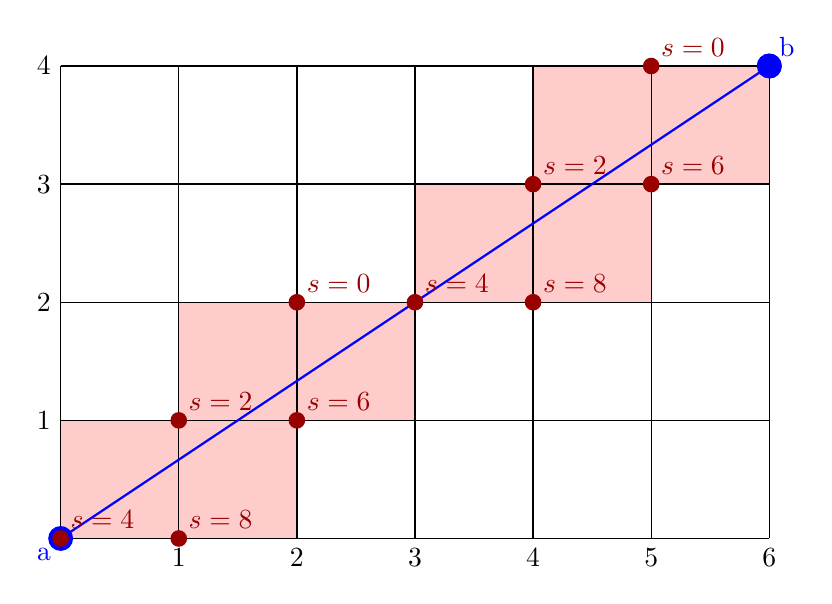
\begin{tikzpicture}[scale=1.5,line width=0.5pt]
    \draw (0,0) grid (6,4);

    \node[below left, blue] at (0,0) {a};
    \node[below] at (1,0) {1};
    \node[below] at (2,0) {2};
    \node[below] at (3,0) {3};
    \node[below] at (4,0) {4};
    \node[below] at (5,0) {5};
    \node[below] at (6,0) {6};

    \node[left] at (0,1) {1};
    \node[left] at (0,2) {2};
    \node[left] at (0,3) {3};
    \node[left] at (0,4) {4};
    \node[above right, blue] at (6,4) {b};
    \fill[blue] (6,4) circle (3pt);

    \filldraw[color=black,fill=red!20] (0,0) rectangle (1,1); 
    \filldraw[color=black,fill=red!20] (1,0) rectangle (2,1);
    \filldraw[color=black,fill=red!20] (1,1) rectangle (2,2);
    \filldraw[color=black,fill=red!20] (2,1) rectangle (3,2);
    \filldraw[color=black,fill=red!20] (3,2) rectangle (4,3); 
    \filldraw[color=black,fill=red!20] (4,2) rectangle (5,3);
    \filldraw[color=black,fill=red!20] (4,3) rectangle (5,4);
    \filldraw[color=black,fill=red!20] (5,3) rectangle (6,4);
    
    \draw[blue, thick] (0,0) -- (6,4);
    \fill[blue] (0,0) circle (3pt);
    \fill[blue] (6,4) circle (3pt);
  
    \node[above right,red!60!black] at (0,0) {$s=4$}; \fill[red!60!black] (0,0) circle (2pt);
    \node[above right,red!60!black] at (1,0) {$s=8$}; \fill[red!60!black] (1,0) circle (2pt);
    \node[above right,red!60!black] at (1,1) {$s=2$}; \fill[red!60!black] (1,1) circle (2pt);
    \node[above right,red!60!black] at (2,1) {$s=6$}; \fill[red!60!black] (2,1) circle (2pt);
    \node[above right,red!60!black] at (2,2) {$s=0$}; \fill[red!60!black] (2,2) circle (2pt);
    \node[above right,red!60!black] at (3,2) {$s=4$}; \fill[red!60!black] (3,2) circle (2pt);
    \node[above right,red!60!black] at (4,2) {$s=8$}; \fill[red!60!black] (4,2) circle (2pt);
    \node[above right,red!60!black] at (4,3) {$s=2$}; \fill[red!60!black] (4,3) circle (2pt);
    \node[above right,red!60!black] at (5,3) {$s=6$}; \fill[red!60!black] (5,3) circle (2pt);
    \node[above right,red!60!black] at (5,4) {$s=0$}; \fill[red!60!black] (5,4) circle (2pt);

  \end{tikzpicture}
  \caption[Line of Sight algorithm]{Cells checked by the Line of Sight algorithm, where $\Delta i = 6$ and $\Delta j = 4$} 
\end{figure}

\section{Query to a bitwise-and-geometrically compressed $LDDB_{N}$}

Figure 3.11 gives an annotated explanation of a query to a bitwise-and-geometrically compressed $LDDB$ using a block size of $3 \times 3$. The steps are elaborated below:

\begin{description}
\item(a) the original query requests the intermediate coordinates on the shortest path between \\ an $ingress$ of $(2,0)$ and an $egress$ of $(3,3)$ on the map shown, i.e. a map of size $3 \times 3$ \\ with integer code 48;
    
\item (b) the integer codes are calculated for all four rotations of the map, and the smallest code \\ is used for the query. The $ingress$ and $egress$ are rotated accordingly;
    
\item (c) the $y-value$ of the rotated $ingress$ coordinate is larger than that of the rotated $egress$ \\ coordinate. Therefore, the $ingress$ and $egress$ are exchanged (i.e. reflected) for the query;
    
\item (d) the final configuration for the query has been reached: map code 18 and \\ $ingress-egress$ coordinates $(3,0)-(0,1)$ which is encoded as $011-000-000-001$;
    
\item (e) the query returns a 64 bit integer, whose 32 most significant bits can be decoded as a {\tt float} \\ giving the length of the shortest path between $ingress$ and $egress$, and whose 24 least significant \\ bits are $010-010-001-010$ which is decoded as $i_{1}=(2,2)$ and $i_{2}=(1,2)$;
    
\item (f) since the coordinates were reflected in step (c), the reflection is undone in step (f). Therefore \\ the first intermediate coordinate $i_{1}=(1,2)$ and the second $i_{2}=(2,2)$;
    
\item (g) since the map was rotated 90$^{\circ}$ clockwise in step (b), the rotation is undone in step (g). \\ Therefore $i_{1}=(1,1)$ and $i_{2}=(1,2)$;
    
\item (h) the result is ready to be returned, which provides {\em Block A*} with the shortest path between \\ the $ingress$ and the $egress$, as shown.
\end{description}

\chapter{Project Proposal}

\vfil

\centerline{\Large \bf Project Proposal}
\vspace{0.4in}
\centerline{\Large A Comparison of Any-Angle Pathfinding Algorithms for Virtual Agents }
\vspace{0.4in}
\centerline{\large O. Freeman, Clare College}
\vspace{0.3in}
\centerline{\large 25$^{th}$ October 2013}
\vspace{0.3in}
\vfil

\noindent
{\bf Project Originator:} O. Freeman
\vspace{0.2in}

\noindent
{\bf Project Supervisor:} Dr. R. J. Gibbens
\vspace{0.2in}

\noindent
{\bf Director of Studies:} Prof. L. J. Paulson
\vspace{0.2in}
\noindent
 
\noindent
{\bf Project Overseers:} Dr.~S.~Clark \& Dr~P.~Li\`o


% Main document

\section*{Introduction}


Finding short and realistic-looking paths through environments with arbitrarily placed obstacles is one of the central problems in artificial intelligence for games and robotics. \\

\noindent
The environment must first be discretised into a graph so that it can be searched. Common discretisation strategies include representing the environment as a grid of blocked and unblocked cells, visibility graphs and navigation meshes. Many algorithms exist to efficiently find optimal paths through graphs, but due to its optimality and efficiency, A* is often the best choice {\em (Nash: 2012)}. However, the paths that A* produces are constrained to travel along the edges of the graph -- in a grid graph, for example, the agent is restricted to travelling at integer multiples of 45$^\circ$. Many discretisation strategies thus produce paths which are longer and have more turns than is necessary, and hence look unnatural to the human eye -- a property that is undesirable when mimicking human behaviour with robots or virtual agents.\\

\noindent
A variety of A*-inspired `any-angle' pathfinding algorithms have been proposed to solve this problem. These include:
\begin{itemize}
\item {\em Post-processing smoothing step to A* (Millington: 2009)} -- collapses multiple straight line segments using a line-of-sight algorithm.
\item {\em Field D* (Ferguson, Stentz: 2006)} -- avoids the constraint of having to travel only to existing nodes by interpolating between g-values to produce new nodes at semi-arbitrary positions.
\item {\em Theta* (Nash, Koenig: 2007)} -- allows nodes to change their parent to certain nodes within line-of-sight.  
\item {\em Block A* (Yap: 2011)} -- performs search on  $N \times N$ cell blocks whose internal optimal paths have been pre-calculated.
\end{itemize}

\noindent
The aim of this project is to compare and contrast the performance of a selection of any-angle pathfinding algorithms. The test suite will consist of randomly generated maps of differing coverage, clustering and grid resolution to ensure that the analysis of the algorithms' properties is suitable for a wide range of application domains.

\vfil

\section*{Starting Point}

My current algorithmic knowledge for this project is:

\begin{itemize}
\item {\em Part 1B CST Artificial Intelligence I} -- A* search.
\item {\em Artificial Intelligence for Games (Millington, Funge)} -- A* pathfinding. 
\end{itemize}

My current programming experience is:

\begin{itemize}
\item {\em Part 1A CST Programming in Java.}
\item {\em Part 1B CST Further Java} and {\em Group Project.}
\item {\em Internship at NaturalMotion Inc.} -– Developed a prototype GUI in Java.
\end{itemize}

\section*{Work to be done}

In order to test and compare the any-angle pathfinding algorithms, I will need to develop an application to generate maps and to run and record the performance of the algorithms. I will also need to use statistical software to evaluate the performance of the algorithms.\\ \\ The project breaks down into the following main sections:


\begin{description}
  \item[Map generation] \hfill \\
  I will develop a tool that can automatically generate maps with adjustable coverage, clustering and resolution. This may require a custom algorithm. The tool will also convert the maps into a search graph.
  \item[Testing simulator] \hfill \\
  I will develop an application that allows me to run one of a collection of algorithms on one of a collection of maps, and then visually display the resulting path and statistics about the path. Therefore the underlying framework must be modular, to allow different maps and algorithms to be used interchangeably.
  \item[Algorithm implementation] \hfill \\
  I will research and implement the any-angle path-finding algorithms.
  \item[Evaluation] \hfill \\
  I will evaluate the performance of the algorithms according to metrics such as:
  
  {\em Path} -- Path length and path straightness. \\
  {\em Graph} -- Clustering, coverage and resolution.\\
  {\em Computation} -- Execution time.
  
\end{description}

\section*{Success Criteria for the Main Result}

The following core components should be produced to declare the project a \\success:

\begin{enumerate}
\item A generator of maps of varying coverage, clustering and resolution.
\item A simulator that can:
\begin{itemize}
\item load one of a collection of maps from the generator;
\item run one of a collection of any-angle path-finding algorithms on the map and display the result visually;
\item return statistics about the performance of the algorithm on the map.
\end{itemize}
\end{enumerate}

\section*{Possible Extensions}

\begin{enumerate}
\item Extend investigation from grid-based map discretization to visibility graphs.

\item Implement a map editor that allows the user to create a custom map by selecting grid locations to be blocked.

\item Adapt the implementation and analyse the performance of the algorithms when the obstacles become traversable with high cost function -- i.e. the agent can climb over the obstacle, but only slowly.

\end{enumerate}

\section*{Resources Required and Backup Strategy}

For this project I shall mainly use my own Macbook Air (1.3GHz dual-core Intel, 4GB RAM, 128GB Disk), with backup provided on cloud storage and version control provided by GitHub. If my computer fails, I will be able to recover my work from the cloud storage and continue my project on the MCS machines.

\vfil

\section*{Timetable: Workplan and Milestones}
Project start date: 28/10/2013.\\

\begin{description}

\item[28$^{th}$ October -- 3$^{rd}$ November (1 week)] \hfill \\

{\em Project set up and familiarization}
\begin{itemize}
\item Start project note book.
\item Set up programming environment, including testing framework.
\item Set up backup strategy.
\end{itemize}
{\em Milestone}: Comfortable with development environment.\\

\item[4$^{th}$ November -- 17$^{th}$ November (2 weeks)] \hfill \\

{\em Literature research and implementation planning}
\begin{itemize}
\item Research and choose any-angle pathfinding algorithms.
\item Research and choose data structures and algorithms that will be necessary for the map generator and algorithm simulator applications.
\item Decide key interfaces of the map generator and algorithm simulator applications.
\end{itemize}
{\em Milestone}: Any-path algorithms chosen and thoroughly understood. Defining features of application identified.\\

\item[18$^{th}$ November -- 15$^{th}$ December (4 weeks)] \hfill \\

{\em Application development phase 1}
\begin{itemize}
\item Devise architecture and class structure, including any design patterns to be used.
\item Implement a prototype simulation application that renders a \\placeholder map and runs a placeholder algorithm. 
\end{itemize}
{\em Milestone}: A working prototype implementation of the simulation application.\\

\item[16$^{th}$ December -- 5$^{th}$ January (3 weeks)] \hfill \\

{\em Application development phase 2}
\begin{itemize}
\item Implement path visualisation in the application.
\item Implement statistical measurement and feedback in the application.
\end{itemize}
{\em Milestone}: Application correctly displays path and path statistics.\\

\item[6$^{th}$ January -- 26$^{th}$ January (3 weeks)] \hfill \\

{\em Path-finding algorithm implementation}
\begin{itemize}
\item Implement and test the chosen any-angle path-finding algorithms.
\end{itemize}
{\em Milestone}: Path-finding algorithms run correctly.\\

\item[27$^{th}$ January -- 9$^{th}$ February (2 weeks)] \hfill \\

{\em Map-generation algorithm implementation}
\begin{itemize}
\item Implement and test the map-generation algorithm.  
\item Test and debug the simulation application.
\end{itemize}
{\em Milestone}: Maps generated according to the input parameters.\\

\item[10$^{th}$ February -- 23$^{rd}$ February (2 weeks)] \hfill \\

{\em Progress report}
\begin{itemize}
\item Write the progress report.  
\item Prepare the presentation.
\item Start gathering data for evaluation.
\end{itemize}
{\em Milestone}: Progress report and presentation complete.\\

\item[24$^{th}$ February -- 9$^{th}$ March (2 weeks)] \hfill \\

{\em Catchup and extension}
\begin{itemize}
\item Learn R - statistical analysis software.
\item Complete any unfinished tasks. 
\item {\em Optional extension 1}: Visibility graph.
\item {\em Optional extension 2}: Custom maps.
\item {\em Optional extension 3}: Traversable obstacles.
\end{itemize}
{\em Milestone}: Code completion.\\

\item[10$^{th}$ March -- 23$^{rd}$ March (2 weeks)] \hfill \\

{\em Dissertation phase 1}
\begin{itemize}
\item Plan the structure of the Dissertation. 
\item Improve \LaTeX\ skills.
\item Write the Preparation chapter.
\item Write the Implementation chapter.
\end{itemize}
{\em Milestone}: Preparation and Implementation chapters complete.\\

\item[24$^{th}$ March -- 13$^{th}$ April (3 weeks)] \hfill \\

{\em Dissertation phase 2}
\begin{itemize}
\item Generate statistics and diagrams.
\item Write the Evaluation chapter.
\end{itemize}
{\em Milestone}: Evaluation chapter complete.\\

\item[14$^{th}$ April -- 27$^{th}$ April (2 weeks)] \hfill \\

{\em Dissertation phase 3}
\begin{itemize}
\item Write the Conclusion.
\item Write the Bibliography and Index.
\item Write the Appendices.
\item Review the Dissertation.
\end{itemize}
{\em Milestone}: Draft Dissertation complete.\\


\item[28$^{th}$ April -- 16$^{th}$ May (2.5 weeks)] \hfill \\

{\em Dissertation phase 4}
\begin{itemize}
\item Complete any unfinished tasks.
\item Refine the Dissertation.
\end{itemize}
{\em Milestone}: Dissertation complete.\\

\end{description}






\end{document}